% Chapter, Section, Theorem, Corollary, Lemma, Definition, Table, Figure, {\bf
\chapter{Turing Machines}\label{ch-11}

In the preceding chapters, we have seen that DFAs and NDFAs represented
the type 3 languages and pushdown automata represented the type 2
languages. In this chapter we will explore the machine analog to
the type 1 and type 0 grammars.  These devices, called \emph{Turing
machines}, are the most powerful automata known and can recognize
every language considered so far in this text. We will also encounter
languages that are too complex to be recognized by any Turing
machine. Indeed, we will see that any other such (finite) scheme
for the representation of languages is likewise forced to be unable
to represent all possible languages over a given alphabet. Turing
machines provide a gateway to \emph{undecidability}, discussed in the next
chapter, and to the general theory of \emph{computational complexity},
which is rich enough to warrant much broader treatment than would
be possible here.

% 11.1 DEFINITIONS AND EXAMPLES
\section{Definitions and Examples}\label{sec-11.1}

Pushdown automata turned out to be the appropriate cognitive devices
for the type 2 languages, but further enhancements in the capabilities
of the automaton model are necessary to achieve the generality
inherent in type 0 and type 1 languages. A (seemingly) minor
modification will be all that is required. \emph{Turing machines} are
comprised of the familiar components that have already been used
in previous classes of automata. As with the earlier constructions,
the heart of the device is a finite-state control, which reacts to
information scanned by the tape head(s).  Like finite-state transducers
and pushdown automata, information can be written\index{read/write head} to tape as
transitions between states are made. Unlike FSTs and PDAs, Turing
machines have only one tape with which to work, which serves both
the input and the output needs of the device. Note that with
finite-state transducers the presence of a second tape was purely
for convenience; a single tape, with input symbols overwritten by
the appropriate output symbol as the read head progressed, would
have sufficed.  Whereas a pushdown automaton could write an entire
string of symbols to the stack, a Turing machine is constrained to
print a single letter at a time.  These new devices would therefore
be of less value than PDAs were they not given some other capability.
In all previous classes of automata, the read head was forced to
move one space to the right on each transition (or, in the case of
$\lambda$-moves, remain stationary).  On each transition, the Turing machine
tape head has the option of staying put, moving right, or moving
left. The ability to move back to the left and review previously
written information accounts for the added power of Turing machines.

It is possible to view a Turing machine as a powerful transducer
of computable functions, with an associated function defined much
like those for FSTs. That is, as with finite-state transducers,
each word that could be placed on an otherwise blank tape is
associated with the word formed by allowing the Turing machine to
operate on that word. With FSTs, this function was well defined;
the machine would process each letter of the word in a unique way,
the read head would eventually find the end of the word (that is,
it would scan a blank), and the device would then halt.  With Turing
machines, there is no built-in guarantee that it will always halt;
since the tape head can move both right and left, it is possible
to define a Turing machine that would reverberate back and forth
between two adjacent spaces indefinitely. A Turing machine is also
not constrained to halt when it scans a blank symbol; it may overwrite
the blank and/or continue moving right indefinitely.

Rather than viewing a Turing machine as a transducer, we will
primarily be concerned with employing it as an acceptor of words
placed on the tape. Some variants of Turing machines are defined
with a set of final states, and the criteria for acceptance would
then be that the device both halt and be in a final state.  For our
purposes, we will employ the writing capabilities of the Turing
machine and simply require that acceptance be indicated by printing
a $\pmb{Y}$ just prior to halting. If such a $\pmb{Y}$ is never printed or the
machine does not halt, the word will be considered rejected.  It
may be that there are words that might be placed on the input tape
that would prevent the machine from halting, which is at best a
serious inconvenience; if the device has been operating for an
extraordinary amount of time, we may not be able to tell if it will
never halt (and thus reject the word), or whether we simply need
to be patient and wait for it to eventually print the $\pmb{Y}$. This
uncertainty can in some cases be avoided by finding a superior
design for the Turing machine, which would always halt, printing $\pmb{N}$
when a word is rejected and $\pmb{Y}$ when a word is accepted. This is not
always a matter of being clever in defining the machine; we will
see that there are some languages that are inherently so complex
that this goal is impossible to achieve.

% Figure 11.1
\begin{figure}[tbh]
\centerline{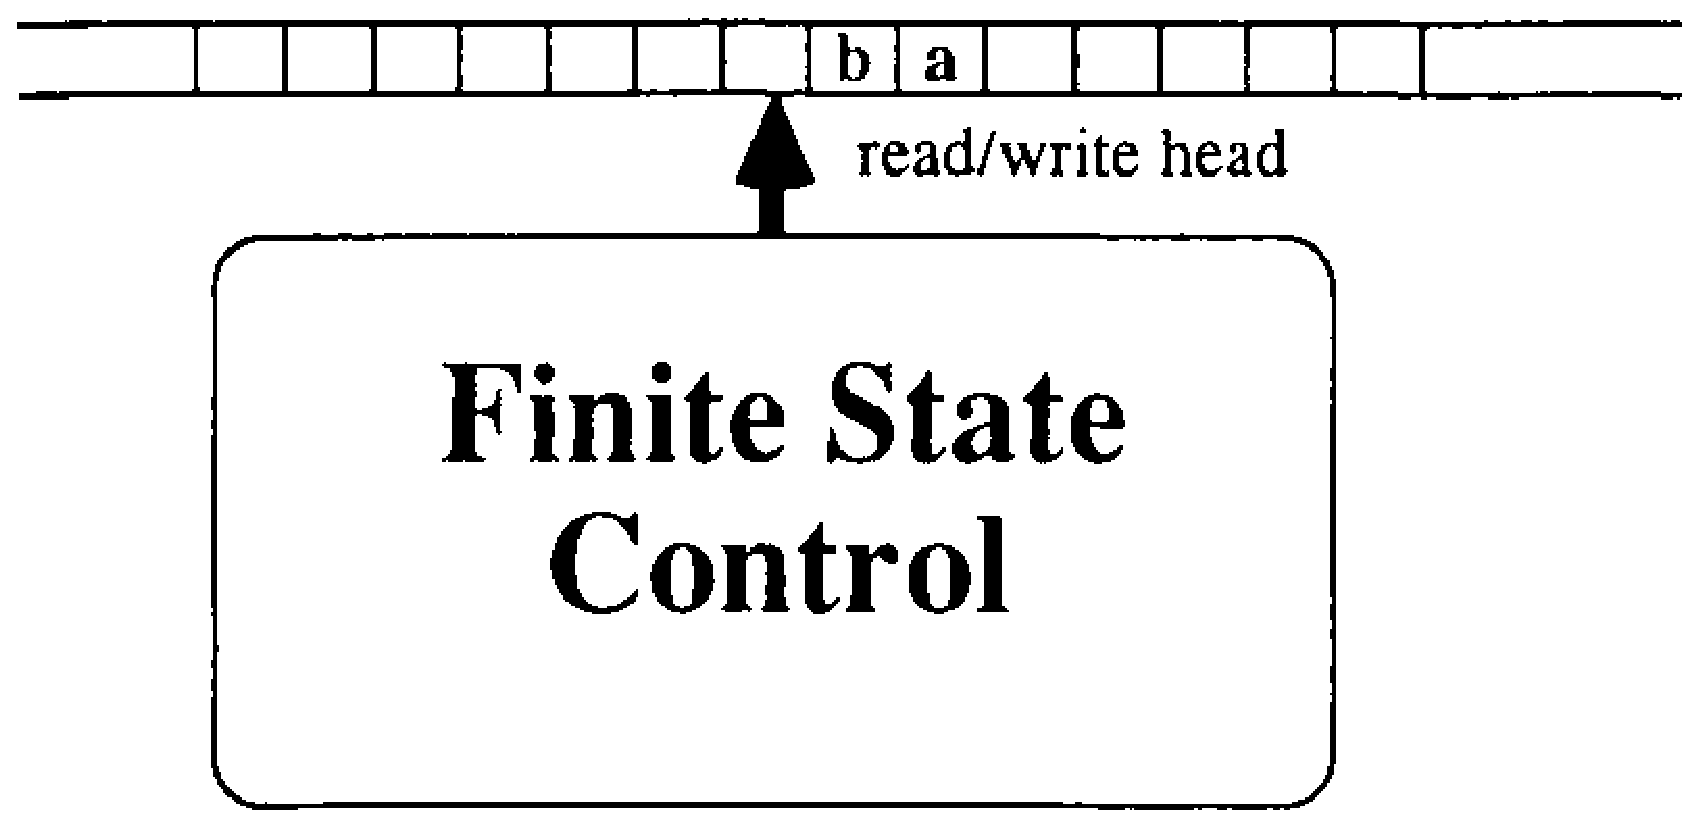
\epsfig{figure=ToFAfigures/fig11-1.eps,width=3.4in}}
\caption{A model of a Turning machine.}\label{fig-11.1}
\end{figure}

A conceptual model of a Turing machine is shown in Figure \ref{fig-11.1}.
Note that the tape head is capable of both reading and overwriting
the currently scanned symbol.  As before, the tape is composed of
a series of cells, with one symbol per cell. The tape head will
also be allowed to move one cell to either the left or right during
a transition. Note that unlike all previous automata, the tape does
not have a ``left end''; it extends indefinitely in both directions.
This tape will be used for input, output, and as a ``scratch pad''
for any intermediate calculations. At the start of operation of the
device, all but a finite number of contiguous cells are blank. Also,
unlike our earlier devices, the following definition implies that
Turing machines may continue to operate after scanning a blank.

% Definition 11.1
\begin{dfn}\label{dfn-11.1}\index{final state!for Turing machine}\index{alphabet!input}\index{alphabet!auxiliary}\index{Turing machine!deterministic}\index{state transition function!for Turing machine}
A \emph{\Index{Turing machine}} that recognizes words over an alphabet $\Sigma$
is a quintuple $M=\langle\Sigma,\Gamma,S,s_0,\delta\rangle$, where

\begin{quote}
$\Sigma$ is the \emph{input alphabet}. \\
$\Gamma$ is the \emph{auxiliary alphabet}, and $\Sigma$, $\Gamma$,
and $\{\pmb{L},\pmb{R}\}$
	are pairwise disjoint sets of symbols. \\
$S$ is a finite nonempty set of \emph{states} (and $S\cap(\Sigma\cup\Gamma) = 
	\emptyset)$. \\
$s_0$ is the \emph{\Index{start state}} $(s_0\in S)$. \\
$\delta$ is the \emph{state transition function} $\delta$: $S\times(\Sigma\cup
	\Gamma)\rightarrow(S\cup\{h\})\times(\Sigma\cup\Gamma\cup\{\pmb{L},\pmb{R}\})$.
\end{quote}
The auxiliary alphabet always includes the \emph{\Index{blank symbol}} (denoted by $\#$),
and neither $\Sigma$ nor $\Gamma$ include the special symbols $\pmb{L}$ and
$\pmb{R}$, which denote moving the tape head left and right, respectively. The
state $h$ is a special \emph{\Index{halt state}}\index{Turing machine!halt state}, from which no further transitions are
possible; $h\notin S$.
\end{dfn}

The alphabet $\Sigma$ is intended to denote the nonblank symbols that can be
expected to be initially present on the input tape. By convention, it is assumed
that the tape head is positioned over the leftmost nonblank (in the case of the
empty string, though, the head will be scanning a blank). In Definition \ref{dfn-11.1},
the state transition function is deterministic; for every state in $S$ and every
tape symbol scanned, exactly one destination state is specified, and one action
is taken by the tape head. The tape head may either:\index{Turing machine!moves}
\begin{enumerate}
\item Overprint the cell with a symbol from $\Sigma$ or $\Gamma$ (and thus a
blank may be printed).
\item Move one cell left (without printing).
\item Move one cell right (also without printing).
\end{enumerate}
In the case where a cell is overprinted, the tape head remains positioned on
that cell.

The above definition of a Turing machine is compatible with the construct
implemented by Jon Barwise and John Etchemendy in their
\Index{Turing's World}$^{\copyright}$ software package for the Apple$^{\text{\textregistered}}$
Macintosh. The Turing's World program allows the user to interactively draw a
state transition diagram of a Turing machine and watch it operate on any given
input string. As indicated by the next example, the same software can be used
to produce and test state transition diagrams for deterministic finite automata.

\subsection*{Example 11.1}

The following simple Turing machine recognizes the set of even-length words
over $\{\pmb{a},\pmb{b}\}$. The state transition diagram for this device is
shown in Figure \ref{fig-11.2} and conforms to the conventions introduced in Chapter \ref{ch-7}.
Transitions between states are represented by arrows labeled by the symbol that
caused the transition. The symbol after the slash denotes the character to be
printed or, in the case of $\pmb{L}$ and $\pmb{R}$, the direction to move the
tape head. The quintuple is $\langle\{\pmb{a},\pmb{b}\},\{\pmb{\#},\pmb{Y},
\pmb{N}\},\{s_0,s_1\},s_0,\delta_T\rangle$, where $\delta_T$ is given by
\begin{center}\begin{tabular}{r@{ = }l}
$\delta_T(s_0,\pmb{a})$ & $\langle s_1,\pmb{R}\rangle$ \\
$\delta_T(s_0,\pmb{b})$ & $\langle s_1,\pmb{R}\rangle$ \\
$\delta_T(s_0,\pmb{\#})$ & $\langle h,\pmb{Y}\rangle$ \\
$\delta_T(s_1,\pmb{a})$ & $\langle s_0,\pmb{R}\rangle$ \\
$\delta_T(s_1,\pmb{b})$ & $\langle s_0,\pmb{R}\rangle$ \\
$\delta_T(s_1,\pmb{\#})$ & $\langle h,\pmb{N}\rangle$
\end{tabular}\end{center}

This particular Turing machine operates in much the same way as a DFA would,
always moving right as it scans each symbol of the word on the input tape.

% Figure 11.2
\begin{figure}
\centerline{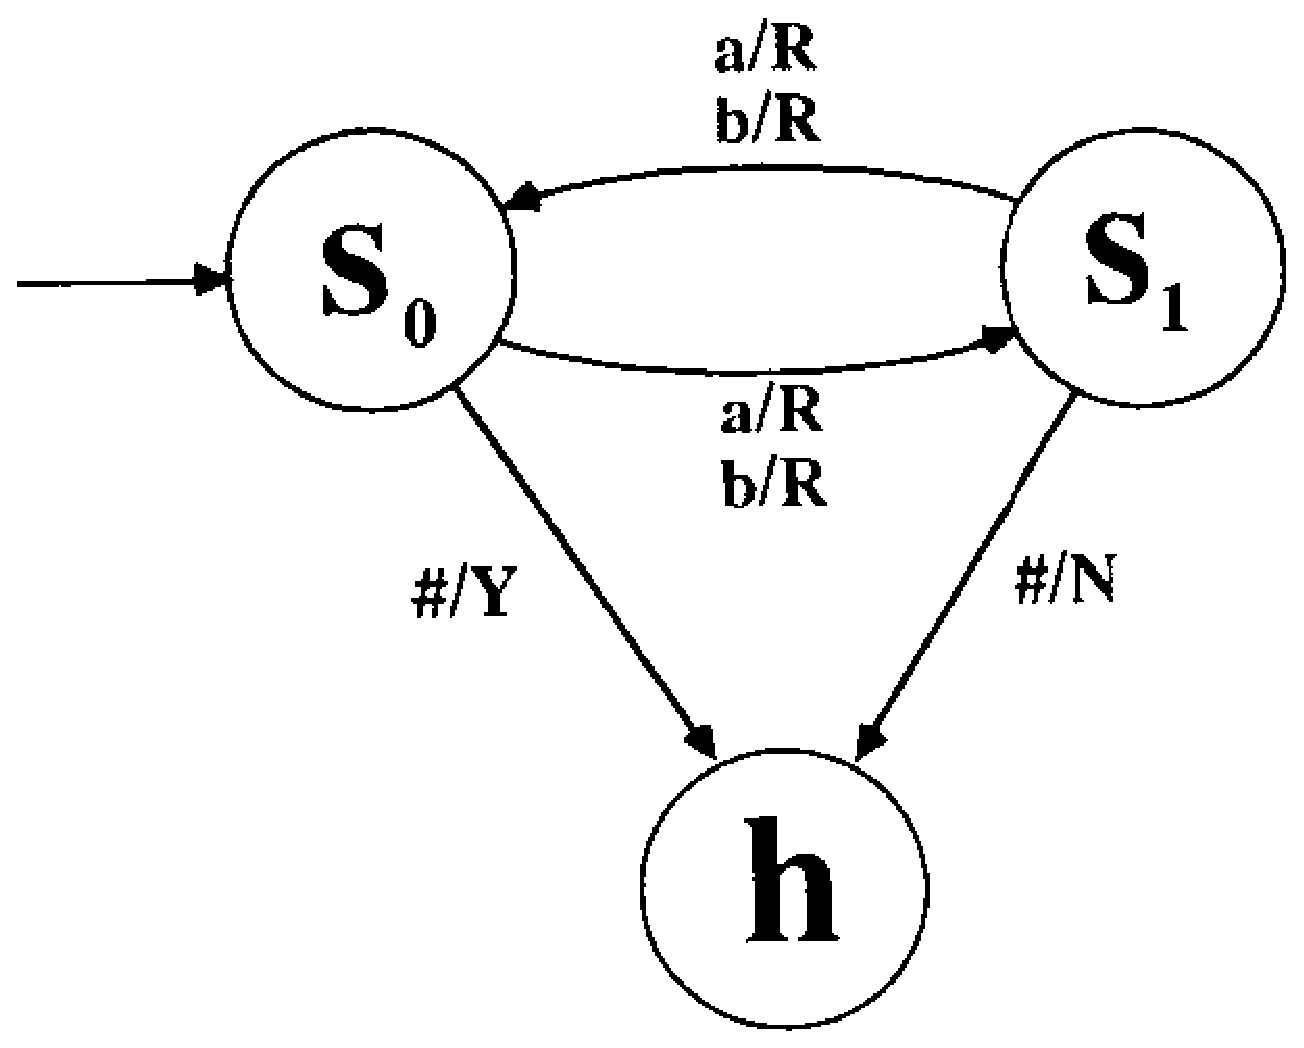
\epsfig{figure=ToFAfigures/fig11-2.eps,width=2.4in}}
\caption{The state transition diagram of the Turing machine discussed in Example
11.1}\label{fig-11.2}
\end{figure}

When it reaches the end of the word (that is, when it first scans a blank), it
prints $\pmb{Y}$ or $\pmb{N}$, depending on which state it is in, and halts. It
differs from a DFA in that the accept/reject indication is printed on the tape
at the right end of the word. Figure \ref{fig-11.3} shows an alternative way of displaying
this machine, in which the halt state is not explicitly shown. Much like the
straight start state arrow that denotes where the automaton is entered, the new
straight arrows show how the machine is left. This notation is especially
appropriate for \emph{\Index{submachines}}. As with complex programs, a complex
Turing machine may be comprised of several submodules. Control may be passed to
a submachine, which manipulates the input tape until it halts. Control may then
be passed to a second submachine, which then further modifies the tape contents.
When this submachine would halt, control may be passed on to a third submachine,
or back to the first submachine, and so on. The straight arrows leaving the
state transition diagram can be thought of as exit arrows for a submachine, and
they function much like a \emph{return} statement in many programming languages.
Example 11.4 illustrates a Turing machine that employs submachines.

% Figure 11.3
\begin{figure}
\centerline{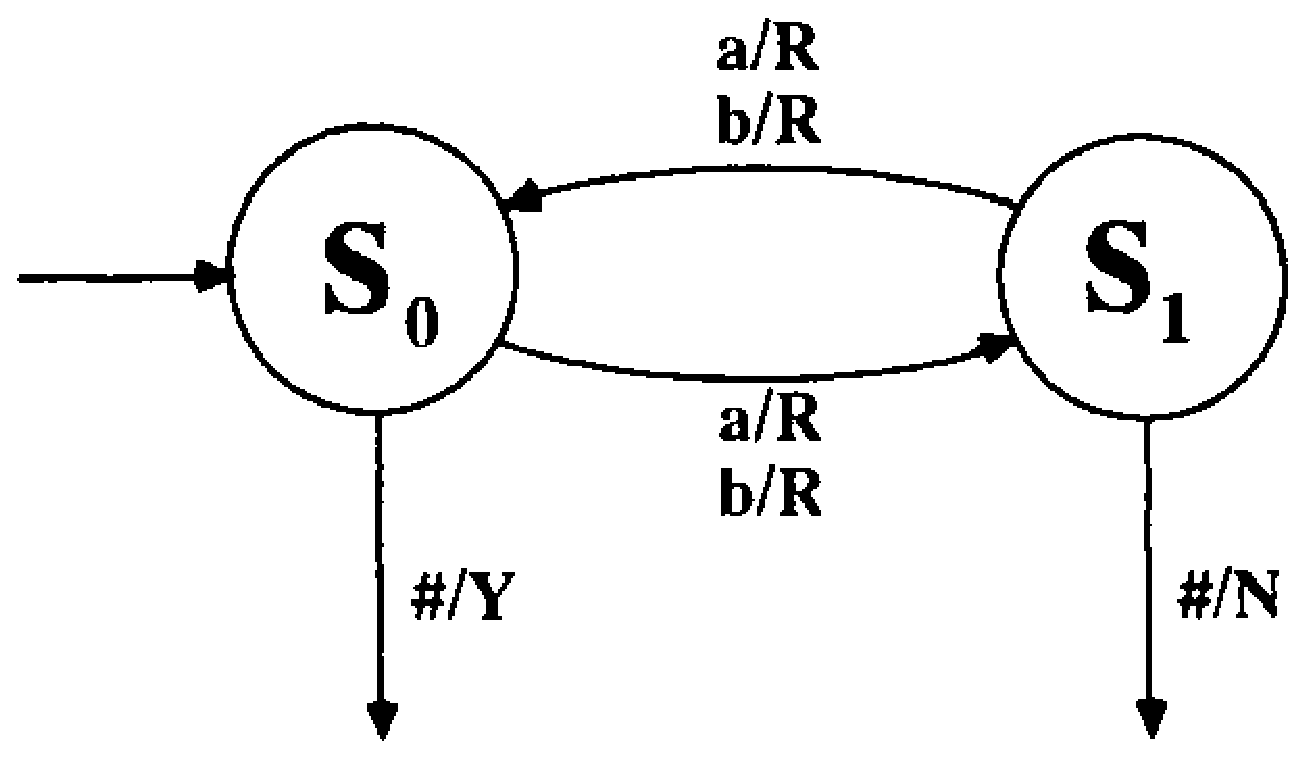
\epsfig{figure=ToFAfigures/fig11-3.eps,width=2.4in}}
\caption{An alternate depiction of the Turing machine discussed in Example 11.1}\label{fig-11.3}
\end{figure}

We will see that any DFA can be emulated by a Turing machine in the manner
suggested by Example 11.1. The following example shows that Turing machines can
recognize languages that are definitely not FAD. In fact, the language accepted
in Example 11.2 is not even context free.

\subsection*{Example 11.2}

The Turing machine $M$ illustrated in Figure \ref{fig-11.4} operates on words over
$\{\pmb{a},\pmb{b},\pmb{c}\}$. When started at the leftmost end of the word, it
is guaranteed to halt at the rightmost end and print $\pmb{Y}$ or $\pmb{N}$. It
happens to overwrite the symbols comprising the input word as it operates, but
this is immaterial. In fact, it is possible to design a slightly more complex
machine that restores the word before halting (see Example 11.11). The quintuple
is $\langle\{\pmb{a},\pmb{b},\pmb{c}\},\{\pmb{\#},\pmb{X},\pmb{Y},\pmb{N}\},\{
s_0,s_1,s_2,s_3,s_4,s_5,s_6\},s_0,\delta\rangle$, where $\delta$ is as indicated
in the diagram in Figure \ref{fig-11.4}. It is intended to recognize the language
$\{x\in\{\pmb{a},\pmb{b},\pmb{c}\}^*|\ \ |x|_{\pmb{a}}=|x|_{\pmb{b}}=|x|_{\pmb{c}}
\}$. One possible procedure for processing a string to check if it had the same
number of $\pmb{a}$s, $\pmb{b}$s, and $\pmb{c}$s is given by the pseudocode
below.

\begin{quote}\begin{tabbing}
aa\=\kill
\emph{while} an $\pmb{a}$ remains \emph{do} \\
\emph{begin} \\
\> replace $\pmb{a}$ by $\pmb{X}$ \\
\> return to leftmost symbol \\
\> find $\pmb{b}$; if none, halt and print $\pmb{N}$ \\
\> replace $\pmb{b}$ by $\pmb{X}$ \\
\> return to leftmost symbol \\
\> find $\pmb{c}$; if none, halt and print $\pmb{N}$ \\
\> replace $\pmb{c}$ by $\pmb{X}$ \\
\> return to leftmost symbol \\
\emph{end} \\
halt and print $\pmb{Y}$ if no more $\pmb{b}$s nor $\pmb{c}$s remain
\end{tabbing}\end{quote}

States $s_0$ and $s_1$ in Figure \ref{fig-11.4} check the \emph{while} condition, and states $s_2$
through $s_6$ perform the body of the do loop. On each iteration, beginning at
the leftmost symbol, state $s_0$ moves the tape head right, checking for symbols
that have not been replaced by $\pmb{X}$. If it reaches the end of the word
(that is, if it scans a blank), the $\pmb{a}$s, $\pmb{b}$s, and $\pmb{c}$s all
matched, and it halts, printing $\pmb{Y}$. If $\pmb{b}$ or $\pmb{c}$ is found,
state 1 searches for $\pmb{a}$s; if the end of the string is reached without
finding a corresponding $\pmb{a}$, the machine halts with $\pmb{N}$, since there
were an insufficient number of $\pmb{a}$s. From either $s_0$ or $s_1$, control
passes to $s_2$ when an $\pmb{a}$ is scanned, and that $\pmb{a}$ is replaced by
$\pmb{X}$. State $s_2$, like $s_4$ and $s_6$, returns the tape head to the
leftmost character. This is done by scanning left until a blank is found and
then moving right as control is passed on to the next state. State $s_3$
searches for $\pmb{b}$, halting with $\pmb{N}$ if none is found. The first
$\pmb{b}$ encountered is otherwise replaced by $\pmb{X}$, and the Turing machine
enters $s_4$, which then passes control on to $s_5$ after returning to the
leftmost symbol. State $s_5$ operates much like $s_3$, searching for $\pmb{c}$
this time, and $s_6$ returns the tape head to the extreme left if the previous
$\pmb{a}$ and $\pmb{b}$ have been matched with $\pmb{c}$. The process then
repeats from $s_0$.

% Figure 11.4
\begin{figure}
\centerline{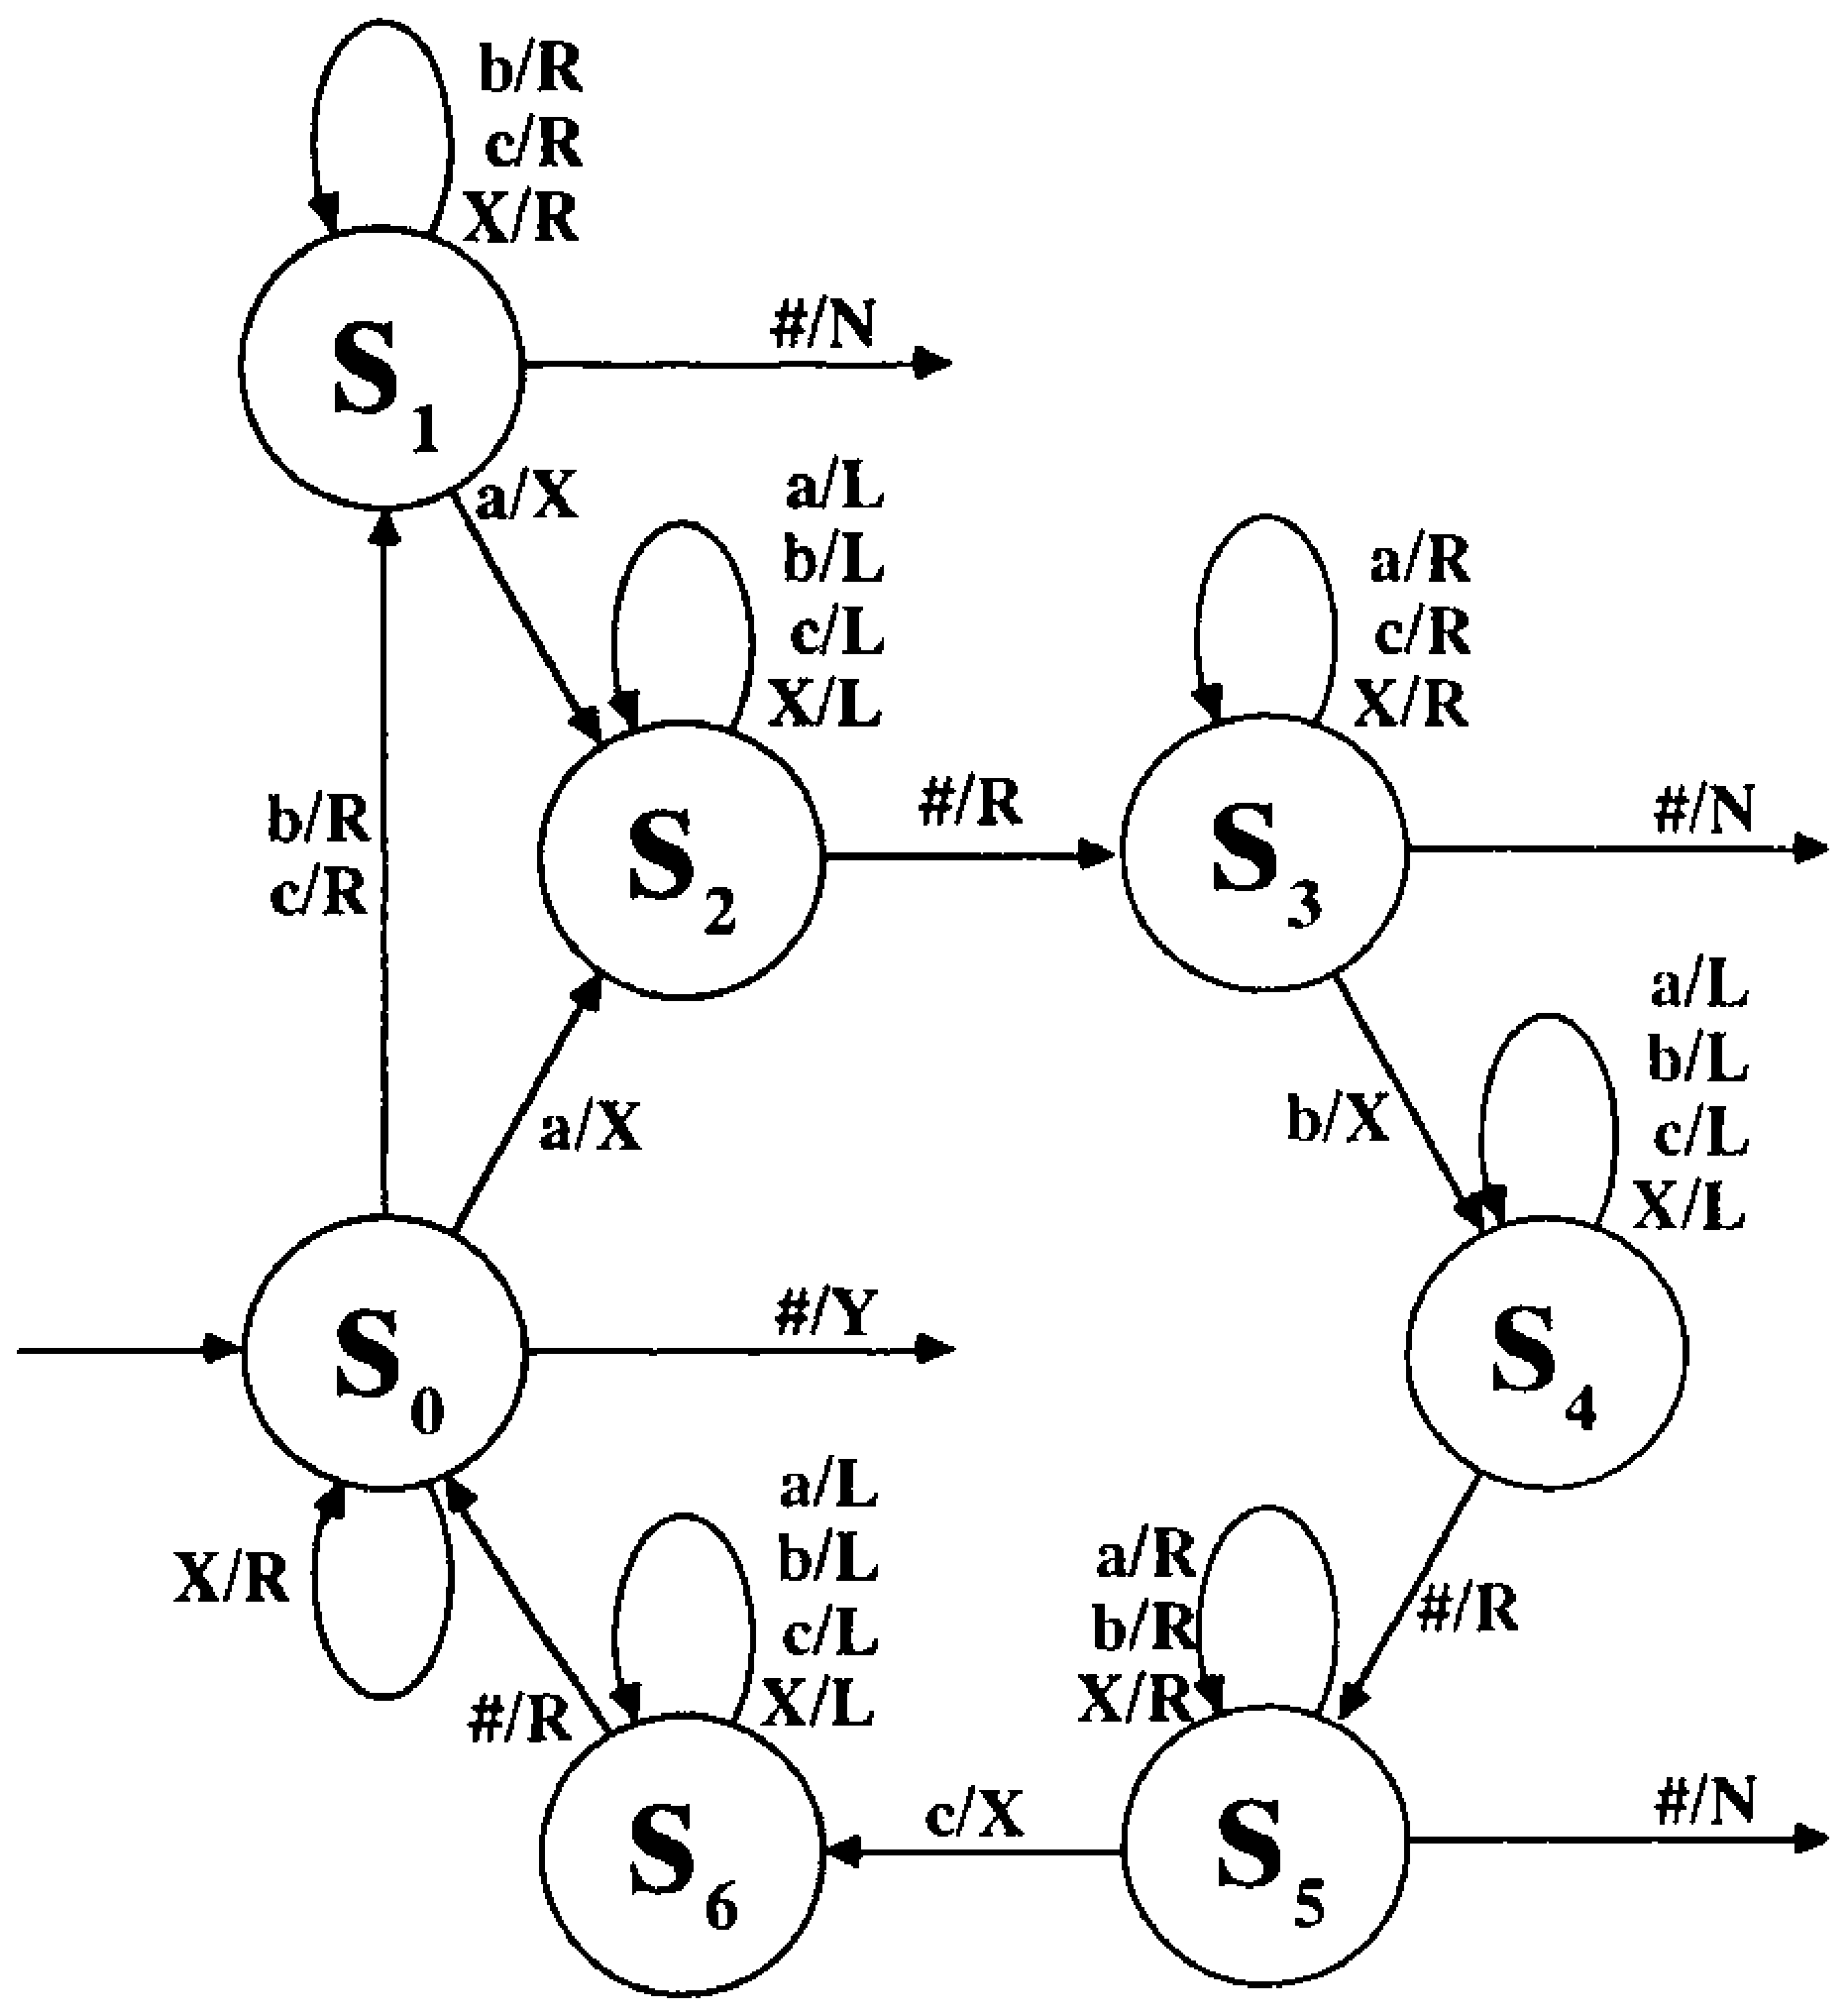
\epsfig{figure=ToFAfigures/fig11-4.eps,height=3.4in}}
\caption{The Turing machine $M$ discussed in Example 11.2}\label{fig-11.4}
\end{figure}

To see exactly how the machine operates, it is useful to step through the
computation for an input string such as $\pmb{babcca}$. To do this, conventions
to designate the status of the device are quite helpful. Like the stack in a
PDA, the tape contents may change as transitions occur, and the notation for the
configuration of a Turing machine must reflect those changes. Steps in a
computation will be represented according to the following conventions.

% Definition 11.2
\begin{dfn}\label{dfn-11.2}\index{Turing machine!configuration}
Let $M=\langle\Sigma,\Gamma,S,s_0,\delta\rangle$ be a Turing machine that is
operating on a tape containing\linebreak$\ldots\pmb{\#\#\#}\alpha\pmb{b}\beta\pmb{\#\#\#}\ldots$,
currently in state $t$ with the tape head scanning the $\pmb{b}$, where $\alpha,
\beta\in(\Sigma\cup\Gamma)^*$, $\alpha$ contains no leading blanks and $\beta$
has no trailing blanks. This configuration will be represented by $\alpha t
\pmb{b}\beta$.

$\gamma\vdash\psi$ will be taken to mean that the configuration denoted by
$\psi$ is reached in one transition from $\gamma$. The symbol $\Dvdash$ will
denote the reflexive and transitive closure of \ $\vdash$.
\end{dfn}

That is, the symbol representing the state will be embedded within the string,
just to the left of the symbol being scanned. If $\delta(t,\pmb{b})=\langle s,
\pmb{R}\rangle$, then $\alpha t\pmb{b}\beta\vdash\alpha\pmb{b} s\beta$. The
new placement of the state label within the string indicates that the tape
head has indeed moved right one symbol. The condition $S\cap(\Sigma\cup\Gamma)=
\emptyset$ ensures that there is no confusion as to which symbol in the
configuration representation denotes the state. As with PDAs, $\gamma\Dvdash\psi$
means that $\gamma$ produces $\psi$ in zero or more transitions. Note that the
leading and trailing blanks are not represented, but $\alpha$ and $\beta$ may
contain embedded blanks. Indeed, $\pmb{b}$ may be a blank. The representation $\pmb{ac\#
\#\#}t\pmb{\#}$ indicates that the tape head has moved past the word $\pmb{ac}$ and is
scanning the fourth blank to the right of the word ($\alpha=\pmb{ac\#\#\#},
\pmb{b}=\pmb{\#},\beta=\lambda$). At the other extreme, $t\pmb{\#\#ac}$ shows
the tape head two cells to the left of the word ($\alpha=\lambda,\pmb{b}=
\pmb{\#},\beta=\pmb{\#ac}$). A totally blank tape\index{tape!blank} is represented by $t\pmb{\#}$.

% Definition 11.3
\begin{dfn}\label{dfn-11.3}\index{language!Turing-acceptable}
For a Turing machine $M=\langle\Sigma,\Gamma,S,s_0,\delta\rangle$, the
\emph{\Index{language accepted by $M$}}, denoted by $L(M)$, is $L(M)=\{x\in
\Sigma^*|\ s_0 x\Dvdash xh\pmb{Y}\}$. A language accepted by a Turing machine is
called a \emph{\Index{Turing-acceptable}} language.
\end{dfn}

It is generally convenient to assume that the special symbol $\pmb{Y}$ is not
part of the input alphabet. Note that words can be rejected if the machine does
not print a $\pmb{Y}$ \emph{or} if the machine never halts.

Several reasonable definitions of acceptance can be applied to Turing machines.
One of the most common specifies that the language accepted by $M$ is the set
of all words for which $M$ simply halts, irrespective of what the final tape
contents are. It might be expected that this more robust definition of
acceptance might lead to more (or at least different) languages being recognized.
However, this definition turns out to yield a device with the same cognitive
power as specified by Definition \ref{dfn-11.3}, as indicated below. More precisely, let
us define
\[ L_1(A) = \{x\in\Sigma^*|\ \exists\alpha,\beta\in(\Sigma\cup\Gamma)^*\ni s_0 x
	\Dvdash \alpha h\beta\} \]
$L_1(A)$ is thus the set of all words that cause $A$ to halt. Let $L$ be a
language for which $L=L_1(B)$ for some Turing machine $B$. It can be shown that
there exists another Turing machine $C$ that accepts $L$ according to Definition
\ref{dfn-11.3}; that is, $L_1(B)=L(C)$ for some $C$. The converse is also true: any
language of the form $L(M)$ is $L_1(A)$ for some Turing machine $A$. Other
possible definitions of acceptance include
\[ L_2(M) = \{x\in\Sigma^*|\ \exists\alpha,\beta\in(\Sigma\cup\Gamma)^*\ni s_0 x
	\Dvdash \alpha h\pmb{Y}\beta\} \]
and
\[ L_3(M) = \{x\in\Sigma^*|\ \exists\alpha\in(\Sigma\cup\Gamma)^*\ni s_0 x\Dvdash
	\alpha h\pmb{Y}\} \]
These distinguish all words that halt with $\pmb{Y}$ somewhere on the tape and
all words that halt with $\pmb{Y}$ at the end of the tape, respectively.

It should be clear that a Turing machine $A_1$, accepting $L=L_1(A_1)$ has an
equivalent\index{equivalent!Turing machines} Turing machine $A_2$ for which $L=L_2(A_2)$. $A_2$ can be obtained
from $A_1$ by simply adding a new state and changing the transitions to the halt
state so that they now all go to the new state. The new state prints $\pmb{Y}$
wherever the tape head is and then, upon scanning that $\pmb{Y}$, halts.
Similarly, a Turing machine $A_3$ can be obtained from $A_2$ by instead
requiring the new state to scan right until it finds a blank. It would then
print $\pmb{Y}$ and halt, and $L_2(A_2)=L_3(A_3)$. The technique for modifying
such an $A_3$ to obtain $A_4$ for which $L_3(A_3)=L(A_4)$ is discussed in the
next section and illustrated in Example 11.11.

\subsection*{Example 11.3}

Consider again the machine $M$ in Example 11.2 and the input string
$\pmb{babcca}$. By the strict definition of acceptance given in Definition \ref{dfn-11.3},
$L(M)=\{\lambda\}$, since $\lambda$ is the only word that does not get destroyed
by $M$. Using the looser criteria for acceptance yields a more interesting
language. The following steps show that $s_0\pmb{babcca}\Dvdash\pmb{XXXXXX}h
\pmb{Y}$.
\begin{center}\begin{tabular}{rllll}
$s_0\pmb{babcca}$ & $\vdash\pmb{b}s_1\pmb{abcca}$ & $\vdash\pmb{b}s_2\pmb{Xbcca}$
	& $\vdash s_2\pmb{bXbcca}$ & $\vdash$ \\
$s_2\pmb{\#bXbcca}$ & $\vdash s_3\pmb{bXbcca}$ & $\vdash s_4\pmb{XXbcca}$ &
	$\vdash s_4\pmb{\#XXbcca}$ & $\vdash$ \\
$s_5\pmb{XXbcca}$ & $\vdash\pmb{X}s_5\pmb{Xbcca}$ & $\vdash\pmb{XX}s_5\pmb{bcca}$
	& $\vdash\pmb{XXb}s_5\pmb{cca}$ & $\vdash$ \\
$\pmb{XXb}s_6\pmb{Xca}$ & $\vdash\pmb{XX}s_6\pmb{bXca}$ & $\vdash\pmb{X}s_6
	\pmb{XbXca}$ & $\vdash s_6\pmb{XXbXca}$ & $\vdash$ \\
$s_6\pmb{\#XXbXca}$ & $\vdash s_0\pmb{XXbXca}$ & $\vdash\pmb{X}s_0\pmb{XbXca}$
	& $\vdash\pmb{XX}s_0\pmb{bXca}$ & $\vdash$ \\
$\pmb{XXb}s_1\pmb{Xca}$ && $\Dvdash s_2\pmb{\#XXbXcX}$ && $\Dvdash$ \\
$\pmb{XX}s_3\pmb{bXcX}$ && $\Dvdash s_4\pmb{\#XXXXcX}$ && $\Dvdash$ \\
$\pmb{XXXX}s_5\pmb{cX}$ && $\Dvdash s_6\pmb{\#XXXXXX}$ && $\Dvdash$ \\
$\pmb{XXXXXX}s_0$ && $\vdash\pmb{XXXXXX}h\pmb{Y}$
\end{tabular}\end{center}
The string $\pmb{babcca}$ is therefore accepted. $\pmb{ac}$ is rejected since
$s_0\pmb{ac}\Dvdash\pmb{Xc}h\pmb{N}$. Further analysis shows that $L_3(M)$ is
exactly $\{x\in\{\pmb{a},\pmb{b},\pmb{c}\}^*|\ \ |x|_{\pmb{a}}=|x|_{\pmb{b}}=
|x|_{\pmb{c}}\}$. Since the only place $\pmb{Y}$ is printed is at the end of the
word on the tape, $L_3(M) = L_2(M)$. Every word eventually causes $M$ to halt
with either $\pmb{Y}$ or $\pmb{N}$ on the tape, and so $L_1(M)=\Sigma^*$.

\subsection*{Example 11.4}\index{parenthesis checker}\index{Turing machine!parenthesis checker}\index{balanced parentheses language}

The composite Turing machine shown in Figure \ref{fig-11.5a} employs two submachines (Figure \ref{fig-11.5b} and Figure \ref{fig-11.5c})
and is based on the parenthesis checker included as a sample in the Turing's
World software. The machine will search for correctly matched parentheses,
restoring the original string and printing $\pmb{Y}$ if the string is
syntactically correct, and leaving a $\pmb{\$}$ to mark the offending position if the
string has mismatched parentheses. Asterisks are recorded to the left of the
string as left parentheses are found, and these are erased as they are matched
with right parentheses.

Figure \ref{fig-11.5a} shows the main architecture of the Turing machine. The square nodes
represent the submachines illustrated in Figures \ref{fig-11.5b} and \ref{fig-11.5c}. When $s_0$
encounters a left parenthesis, it marks the occurrence with $\pmb{\$}$, and
transfers control to the submachine $S_1$. $S_1$ moves the read head to the left
end of the string, and deposits one $\pmb{^*}$ there. The cells to the left of the
original string serve as a scratch area; the asterisks record the number of
unmatched left parentheses encountered thus far. Submachine $S_1$ then scans
right until the $\pmb{\$}$ is found; it then restores the original left
parenthesis. At this point, no further internal moves can be made in $S_1$, and
the arrow leaving $s_{12}$ indicates that control should be returned to the
parent automaton.

The transition leaving the square $S_1$ node in Figure \ref{fig-11.5a} now applies, and
the tape head moves to the right of the left parenthesis that was just processed
by $S_1$, and control is returned to $s_0$. $s_0$ continues to move right past
the symbols $\pmb{a}$ and $\pmb{b}$, uses $S_1$ to process subsequent left
parenthesis, and transfers control to the submachine $S_2$ whenever a right
parenthesis is encountered.

Submachine $S_2$ attempts to match a right parenthesis with a previous left
parenthesis. As control was passed to $S_2$, the right parenthesis was replaced
by $\pmb{\$}$ so that this spot on the tape can be identified later. The
transitions in state $s_{20}$ move the tape head left until a blank cell is
scanned. If the cell to the right of this blank does not contain an asterisk,
$s_{21}$ has no moves and control is passed back to the parent Turing machine,
which will enter $s_4$ and move right past all the symbols in the word, printing
$\pmb{N}$ as it halts. The absence of the asterisk implies that no previous
matching left parenthesis had been found, so halting with $\pmb{N}$ is the
appropriate action.

If an asterisk had been found, $s_{21}$ would have replaced it with a blank, and
then would have no further moves, and the return arrow would be followed. The
blank that is now under the tape head will cause the parent automaton to pass
control to $s_3$, which will move right to $ \pmb{\$}$, and the $\pmb{\$}$ is
then restored to $\pmb{)}$. Control returns to $s_0$ as the tape head moves past
this parenthesis.

The start state continues checking the remainder of the word in this fashion.
When the end of the word is reached, $s_6$ is used to examine the left end of
the string; remaining asterisks indicate unmatched left parentheses, and will
yield $\pmb{N}$ as the machine halts from $s_8$. If $s_6$ does not encounter
$\pmb{^*}$, the Turing machine halts with $\pmb{Y}$ and accepts the string from
$s_7$.
\setcounter{figure}{0}
\renewcommand{\thefigure}{\arabic{chapter}.5\alph{figure}}
% Figure 11.5a
\begin{figure}
\centerline{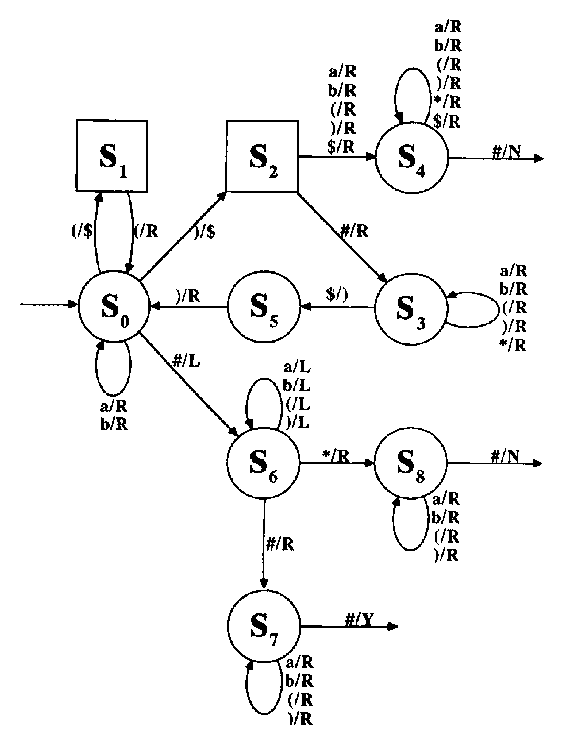
\epsfig{figure=ToFAfigures/fig11-5a.eps,height=4.0in}}
\caption{The Turing machine discussed in Example 11.4}\label{fig-11.5a}
\end{figure}

% Figure 11.5b
\begin{figure}
\centerline{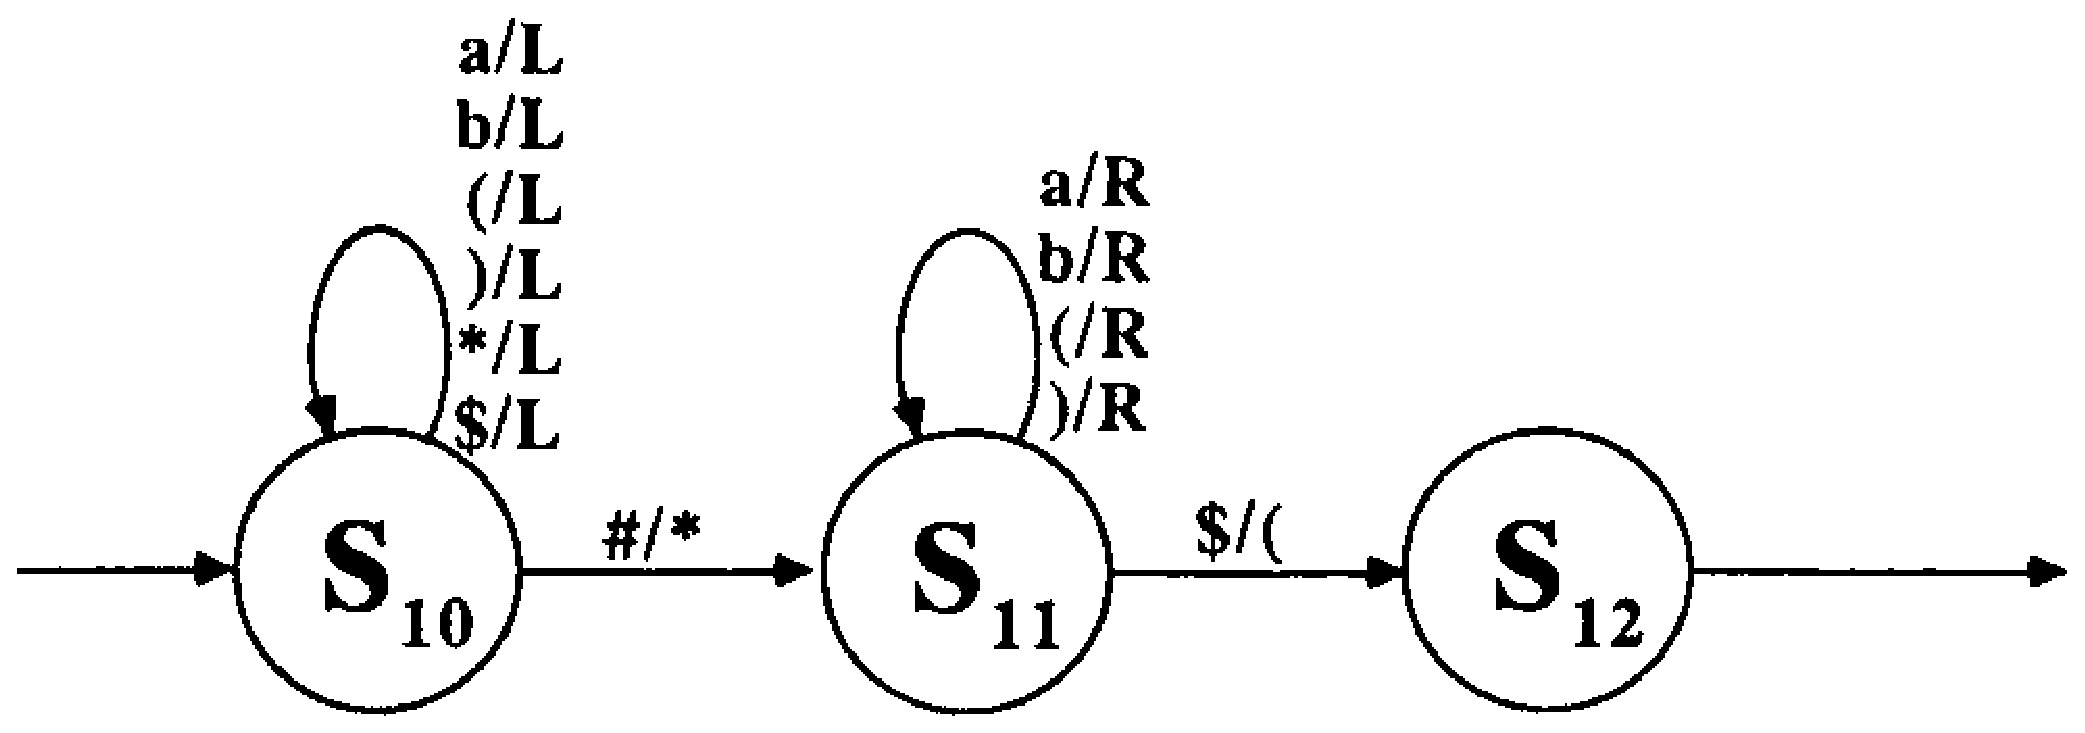
\epsfig{figure=ToFAfigures/fig11-5b.eps,height=1.2in}}
\caption{Submachine $S_1$ in Example 11.4}\label{fig-11.5b}
\end{figure}

% Figure 11.5c
\begin{figure}
\centerline{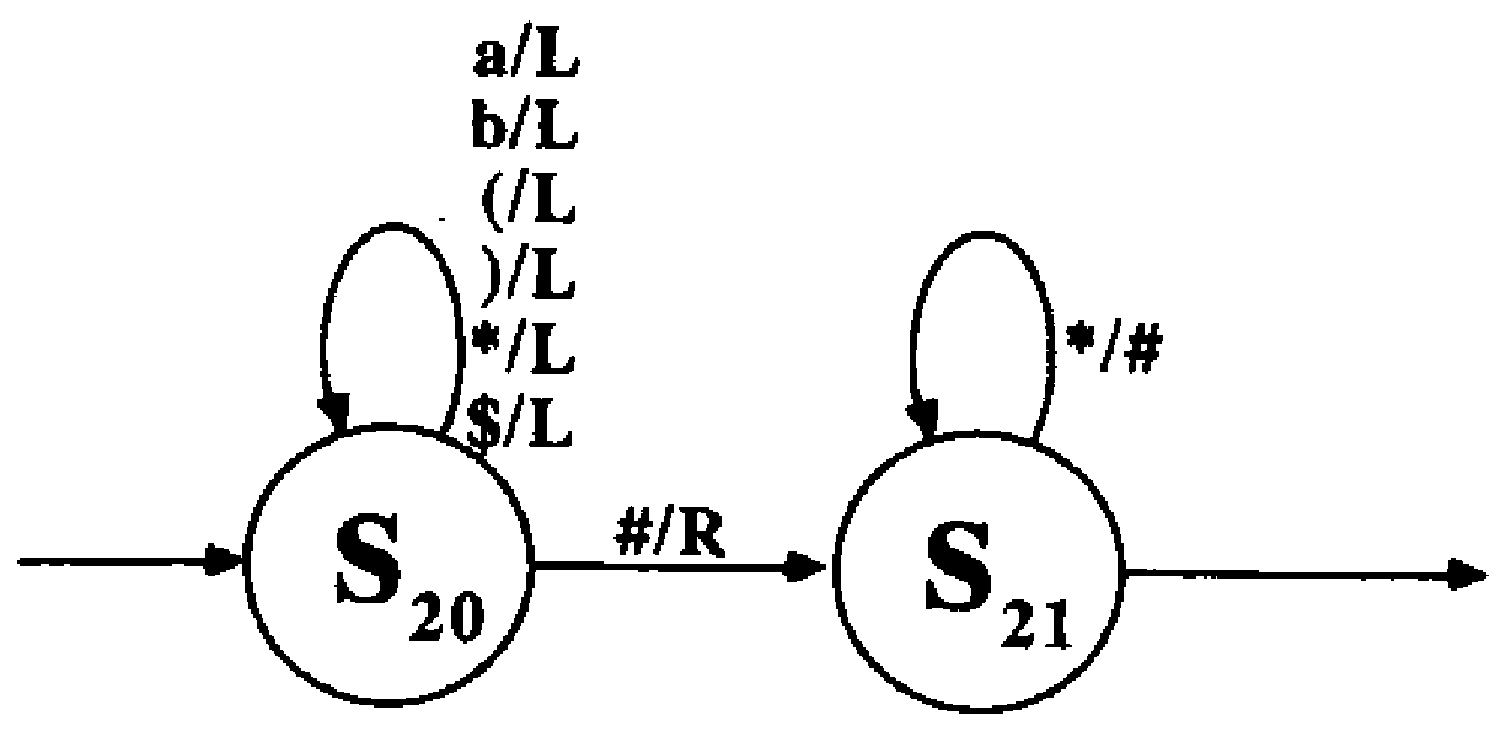
\epsfig{figure=ToFAfigures/fig11-5c.eps,height=1.2in}}
\caption{Submachine $S_2$ in Example 11.4}\label{fig-11.5c}
\end{figure}
\setcounter{figure}{5}                        %nasty kluge
\renewcommand{\thefigure}{\arabic{chapter}.\arabic{figure}}

As more complex examples are considered, one may begin to suspect that any
programming assignment could be carried out on a Turing machine. While it would
be truly unwise to try to make a living selling computers with this architecture,
these devices are generally regarded to be as powerful as any general-purpose
computer. That is, if an algorithm for solving a class of problems can be
carried out on a computer, then there should be a Turing machine that can
produce identical output for each instance of a problem in that class.

The language $\{x\in\{\pmb{a},\pmb{b},\pmb{c}\}^*|\ \ |x|_{\pmb{a}}=|x|_{\pmb{b}}
=|x|_{\pmb{c}}\}$ is not context free, so it cannot be recognized by a PDA.
Turing machines can therefore accept some languages that PDAs cannot, and we
will see that they can recognize every context-free language. We began with DFAs,
which were then extended to the more powerful PDAs, which have now been eclipsed
by the Turing machine construct. Each of these classes of automata has been
substantially more capable than the previous class. If this text were longer,
one might wonder when the next class of superior machines would be introduced.
Barring the application of magic or divine intuition, there does not seem to be
a ``next class.'' That is, any machine that is constrained to operate
algorithmically by a well-defined set of rules appears to have no more computing
power than do Turing machines.

This constraint, ``to behave in an algorithmic fashion,'' is an intuitive notion
without an obvious exact formal expression. Indeed, ``behaving like a Turing
machine'' is generally regarded as the best way to express this notion! A
discussion of how Turing machines came to be viewed in this manner is perhaps in
order. An excellent in-depth treatment of their history can be found in [BARW].

At the beginning of the twentieth century, mathematicians were searching for a
universal algorithm that could be applied to mechanically prove any well-stated
mathematical formula. This naturally focused attention on the manipulation of
symbols. In 1931, G\"odel showed that algorithms of this sort cannot exist. Since
this implied that there were classes of problems that could not have an
algorithmic solution, this then led to attempts to characterize those problems
that could be effectively ``computed.'' In 1936, Turing introduced his formal
device for symbol manipulation and suggested that the definition of an algorithm
be based on the Turing machine. He also outlined the \emph{halting problem}\index{halting problem!for Turing machines}\index{Turing machine!halting problem}
(discussed later), which demonstrated a problem to which no Turing
machine could possibly provide the correct answer in all instances. The search
for a better, perhaps more powerful characterization of what constitutes an
algorithm continued.

While it cannot be proved that it is impossible to find a better formalization
that is truly more powerful, on the basis of the accumulating evidence, no one
believes that a better formulation exists. For one thing, other attempts at
formalization, including grammars, $\lambda$-calculus, $\mu$-recursive
functions, and Post systems, have all turned out to yield exactly the same
computing power as Turing machines. Second, all attempts at ``improving'' the
capabilities of Turing machines have not expanded the class of languages that
can be recognized. Some of these possible improvements will be examined in the
next section. We close this section by formalizing what Example 11.1 probably
made clear: every DFA can be simulated by a Turing machine.

% Theorem 11.1
\begin{thm}\label{thm-11.1}\index{equivalent!Turing machines}
Every FAD language is Turing acceptable.

\emph{Proof.} We show that given any DFA $A=\langle\Sigma,S,s_0,\delta,F
\rangle$, there is a Turing machine $M_A$ that is equivalent to $A$. Define
$M_A=\langle\Sigma,\{\pmb{\#},\pmb{Y},\pmb{N}\},S,s_0,\delta_A\rangle$, where
$\delta_A$ is defined by
\begin{center}\begin{tabular}{r@{ = }l}
$(\forall s\in S)(\forall\pmb{a}\in\Sigma)(\delta_A(s,\pmb{a})$ & $\langle
	\delta(s,\pmb{a}),\pmb{R}\rangle)$ \\
$(\forall s\in F)(\delta_A(s,\pmb{\#})$ & $\langle h,\pmb{Y}\rangle)$ \\
$(\forall s\in S-F)(\delta_A(s,\pmb{\#})$ & $\langle h,\pmb{N}\rangle)$
\end{tabular}\end{center}
A simple inductive argument on $|x|$ shows that
\[ (\forall x\in\Sigma^*)(\forall\alpha,\beta\in(\Sigma\cup\Gamma)^*)(\alpha tx 
	\beta\Dvdash \alpha xq\beta\text{ iff }\DBAR_A(t,x) = q) \]
From this it follows that
\[ (\forall x\in\Sigma^*)(s_0x\Dvdash xq\pmb{\#}\text{ iff }\DBAR_A(s_0,x)=q) \]
Therefore,
\[ (\forall x\in\Sigma^*)(s_0x\Dvdash xh\pmb{Y}\text{ iff }\DBAR_A(s_0,x)\in
	F) \]
which means that $L(M_A)=L(A)$.
\end{thm}

This result actually follows trivially from the much stronger results presented
later. Not only is every type 3 language Turing acceptable, but every type 0
language is Turing acceptable (as will be shown by Theorem \ref{thm-11.2}). The above
proof presents the far more straightforward conversion available to type 3
languages and illustrates the flavor of the inductive arguments needed in other
proofs concerning Turing machines. By using this conversion, the  \Index{Turing's World}$^{\copyright}$
software can be employed to interactively build and test deterministic finite
automata on the Apple$^{\text{\textregistered}}$ Macintosh.

\subsection*{Example 11.5}

Consider the DFA $T$ shown in Figure \ref{fig-11.6}, which recognizes all words of even
length over $\{\pmb{a},\pmb{b}\}$. The corresponding Turing machine is
illustrated in Example 11.1 (see Figure \ref{fig-11.2}).

% Figure 11.6
\begin{figure}
\centerline{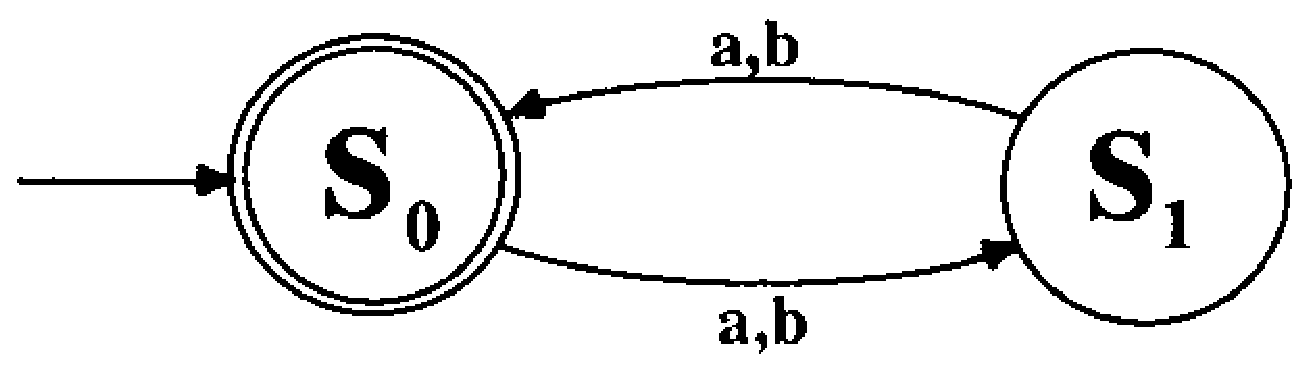
\epsfig{figure=ToFAfigures/fig11-6.eps,width=2.4in}}
\caption{The DFA $T$ discussed in Example 11.5}\label{fig-11.6}
\end{figure}

\section{Variants of Turing Machines}\label{sec-11.2}

There are several ways in which the basic definition of the Turing machine can
be modified. For example, Definition \ref{dfn-11.1} disallows the tape head from both
moving and printing during a single transition. It should be clear that if such
an effect were desired at some point it could be effectively accomplished under
the more restrictive Definition \ref{dfn-11.1} by adding a state to the finite-state
control. The desired symbol could be printed as control is transferred to the
new state. The transition out of the new state would then move the tape head in
the appropriate fashion, thus accomplishing in two steps what a ``fancier''
automaton might do in one step. While this modification might be convenient,
the ability of Definition \ref{dfn-11.1}-style machines to simulate this behavior makes it
clear that such modified automata are no more powerful than those given by
Definition \ref{dfn-11.1}. That is, every such modified automaton has an equivalent Turing
machine.\index{equivalent!Turing machines}

It is also possible to examine machines that are more restrictive than
Definition \ref{dfn-11.1}. If the machine were constrained to write on only a fixed,
finite amount of the tape, this would seriously limit the types of languages
that could be recognized. In fact, only the type 3 languages can be accepted by
such machines.  \emph{Linear bounded automata}, \index{linear bounded automaton} which are Turing machines
constrained to write only on the portion of the tape containing the original
input word, are also less powerful than unrestricted Turing machines and are
discussed in a later section. Having an unbounded area in which to write is
therefore an important factor in the cognitive power of Turing machines, but it
can be shown that the tape need not be unbounded in both directions.\index{Turing machine!bounded on one end} That is,
Turing machines that cannot move left of the cell the tape head originally
scanned can perform any calculation that can be carried out by the
less-restrictive machines given by Definition \ref{dfn-11.1} (see the exercises).

In deciding whether a Turing machine can simulate the modified machines
suggested below, it is important to remember that the auxiliary alphabet
$\Gamma$ can be expanded as necessary, as long as it remains finite. In
particular, it is possible to expand the information content of each cell by
adding a second ``track'' to the tape. For example, we may wish to add check
marks to certain designated cells, as shown in Figure \ref{fig-11.7}. The lower track
would contain the original symbols, and the upper track mayor may not have a
check mark. This can be accomplished by doubling the combined size of the
alphabets $\Sigma$ and $\Gamma$ to include all symbols without check marks and
the same symbols with check marks. The new symbols can be thought of as ordered
pairs, and erasing a check mark then amounts to rewriting a pair such as
$\langle\pmb{a},\sqrt{}\rangle$ with $\langle\pmb{a},\pmb{\#}\rangle$. A scheme
such as this could be used to modify the automaton in Example 11.2. Rather than
replacing designated symbols with $\pmb{X}$, a check could instead be placed
over the original symbol. Just prior to acceptance, each check mark could be
erased, leaving the original string to the left of the $\pmb{Y}$ (see Example
11.11).

% Figure 11.7
\begin{figure}\index{multi-track Turing machine}\index{Turing machine!multi-track}
\centerline{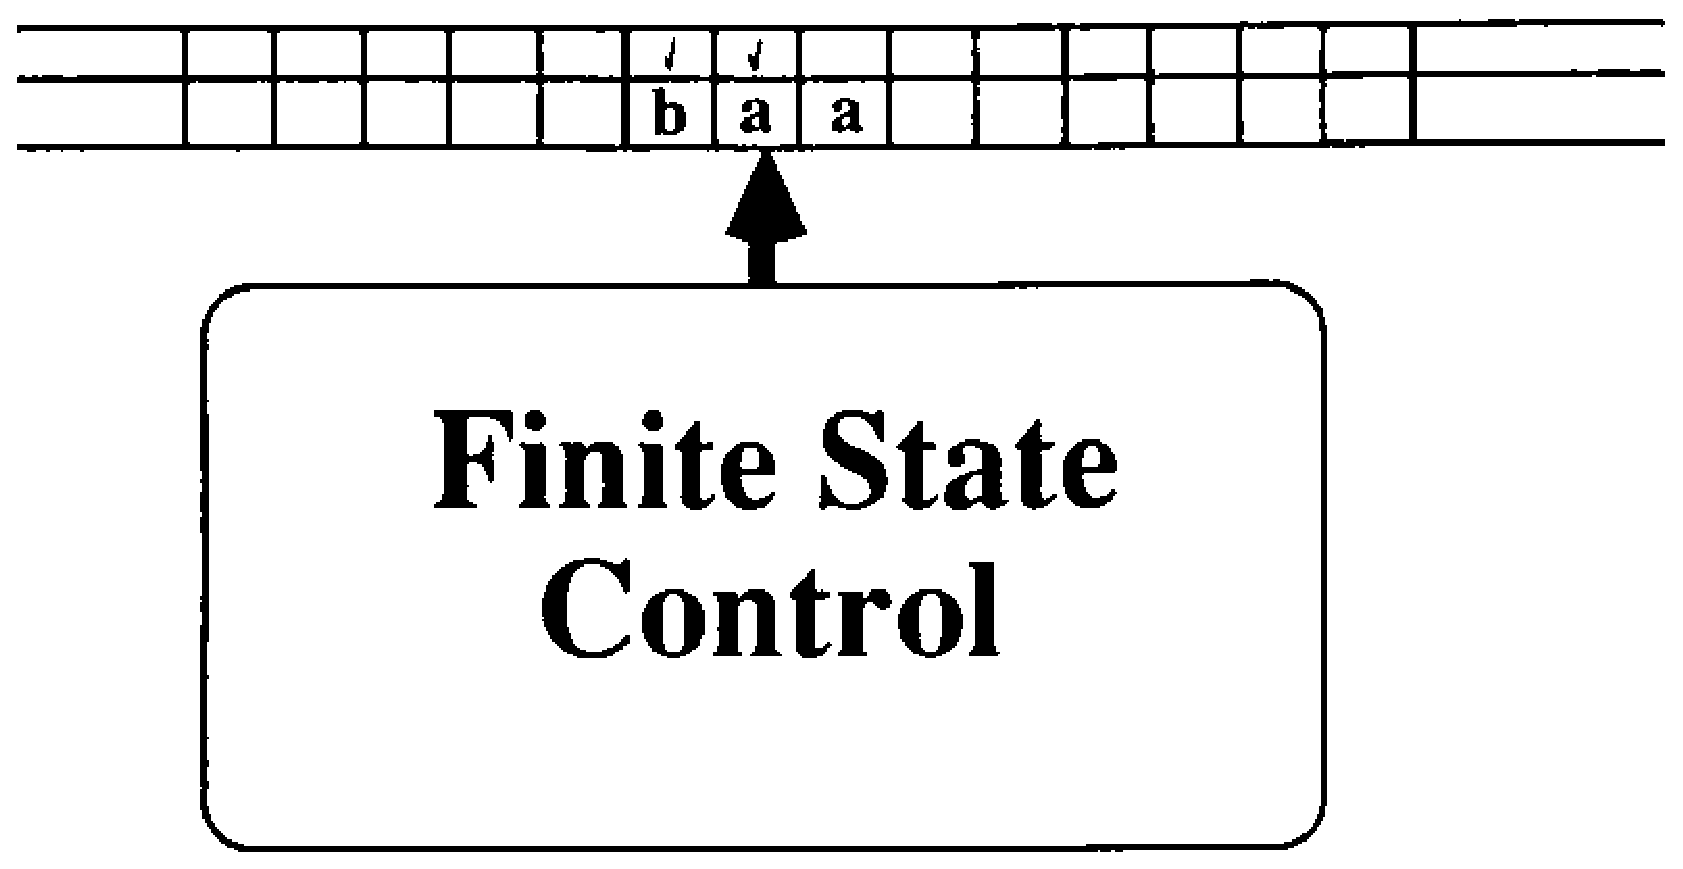
\epsfig{figure=ToFAfigures/fig11-7.eps,width=3.4in}}
\caption{A Turing machine with a two-track tape}\label{fig-11.7}
\end{figure}
 
The foregoing discussion justifies that a Turing machine with a tape head
capable of reading two tracks can be simulated by a Definition \ref{dfn-11.1} style Turing
machine; indeed, it \emph{is} a Turing machine with a slightly more complex alphabet.
When convenient, then, we may assume that we have a Turing machine with two
tracks. A similar argument shows that, for any finite number $k$, a $k$-track
machine has an equivalent\index{equivalent!Turing machines} one-track Turing machine with an expanded alphabet.
The symbols on the other tracks can be more varied than just $\sqrt{}$ and
$\pmb{\#}$; any finite number of symbols may appear on any of the tracks.
Indeed, a Turing machine may initially make a copy of the input string on another
track to use in a later calculation and/or to restore the tape to its original
form. The ability to preserve the input word in this manner illustrates why each
language $L=L_3(A)$ for some Turing machine $A$ must be Turing acceptable; that
is, $L=L_3(A)$ implies that there is a multitrack Turing machine $M$ for which
$L=L(M)$.

\subsection*{Example 11.6}\index{tape!multi-track}

Conceptualizing the tape as being divided into tracks simplifies many of the
arguments concerning modification of the basic Turing machine design. For
example, a modified Turing machine might have two heads that move independently
up and down a single tape, both scanning symbols to determine what transition
should be made and both capable of moving in either direction (or remaining
stationary and overwriting the current cell) as each transition is carried out.
Such machines would be handy for recognizing certain languages. The set
$\{\pmb{a}^n\pmb{b}^n| n\geq 1\}$ can be easily recognized by such a machine.
If both heads started at the left of the word, one head might first scan right
to the first $\pmb{b}$ encountered. The two heads could then begin moving in
unison to the right, comparing symbols as they progressed, until the leading
head encounters a blank and/or the trailing head scans its first $\pmb{b}$. If
these two events occurred on the same move, the word would be accepted. A single
head Turing machine would have to travel back and forth across the word several
times to ascertain if it contained the same number of $\pmb{a}$s as $\pmb{b}$s.
The ease with which the two-headed mutation accomplished the same task might
make one wonder whether such a modified machine can recognize any languages
which the standard Turing machine cannot.

% Figure 11.8
\begin{figure}
\centerline{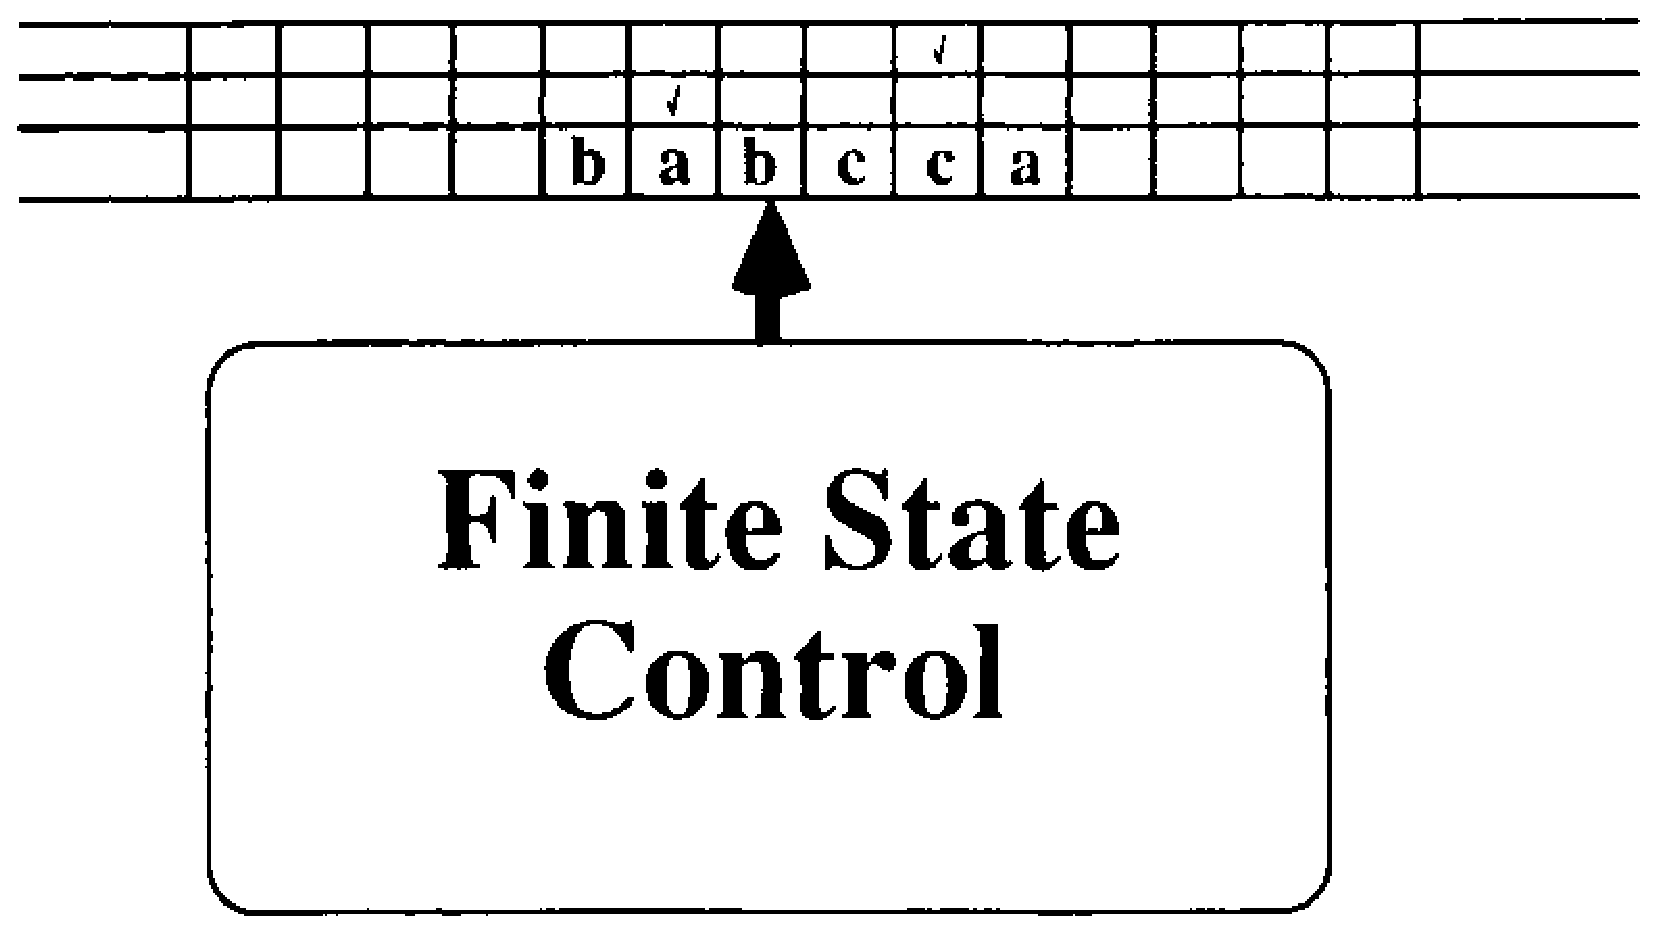
\epsfig{figure=ToFAfigures/fig11-8.eps,width=3.4in}}
\caption{Emulating a two-headed Turing machine with a three-track tape}\label{fig-11.8}
\end{figure}

To justify that a two-headed Turing machine is no more powerful than the type
described by Definition \ref{dfn-11.1}, we must show that any two-headed machine can be
simulated by a corresponding standard Turing machine. As suggested by Figure
\ref{fig-11.8}, a three-track Turing machine will suffice. The original information would
remain on the first track, and check marks will be placed on tracks 2 and 3 to
signify the simulated locations of the two heads. Several moves of the single
head will be necessary to simulate just one move of the two-headed variant, and
the finite-state control must be replicated and augmented to keep track of the
stages of the computation. Each simulated move will begin with the single tape
head positioned over the leftmost check mark. The tape contents are scanned, and
the symbol found is remembered by the finite state control. The tape head then
moves right until the second check mark is found. At this point, the device will
have available the input symbols that would have been scanned by both heads in
the two-headed variant, and hence it can determine what action each of the heads
would have taken. The rightmost checkmark would then be moved left or right or
the current symbol on track 1 overwritten, whichever is appropriate. The single
tape head would then scan left until the other check mark is found, which would
then be similarly updated. This would complete the simulation of one move, and
the process would then repeat.

Various special cases must be dealt with carefully, such as when both heads
would be scanning the same symbol and when the heads ``cross'' to leave a
different head as the leftmost. These cases are tedious but straightforward to
sort out, and thus any language that can be recognized by a two-headed machine
can be recognized by a standard Turing machine. Similarly, a $k$-headed Turing
machine can be simulated by a machine conforming to Definition \ref{dfn-11.1}. The number
of tracks required would then be $k+1$, and the set of states must expand so
that the device can count the number of check marks scanned on the left and
right sweeps of the tape.

Multihead Turing machines are therefore fundamentally no more powerful than the
single-head variety. This means that whenever we need to justify that some task
can be accomplished by a Turing machine we may employ a variant with several
heads whenever this is convenient. We have seen that this variant simplified the
justification that $\{\pmb{a}^n\pmb{b}^n|n\geq 1\}$ was Turing acceptable. It
can also be useful in showing that other variants are no more powerful than the
type of machines given by Definition \ref{dfn-11.1}, as illustrated in the next example.

\subsection*{Example 11.7}

Consider now a device employing several independent tapes with one head for each
tape, as depicted in Figure \ref{fig-11.9}. If we think of the tapes as stationary and the
heads mobile, it is easy to see that we could simply glue the tapes together
into one thick tape with several tracks, as indicated in Figure \ref{fig-11.10}. The
multiple heads would now scan an entire column of cells, but a head would
ignore the information on all but the track for which it was responsible. In
this fashion, a multitape Turing machine can be simulated by a multihead Turing
machine, which can in turn be simulated by a standard Turing machine. Thus,
multitape machines are no more powerful than the machines considered earlier.

% Figure 11.9
\begin{figure}\index{multi-head Turing machine}\index{Turing machine!multi-head}
\centerline{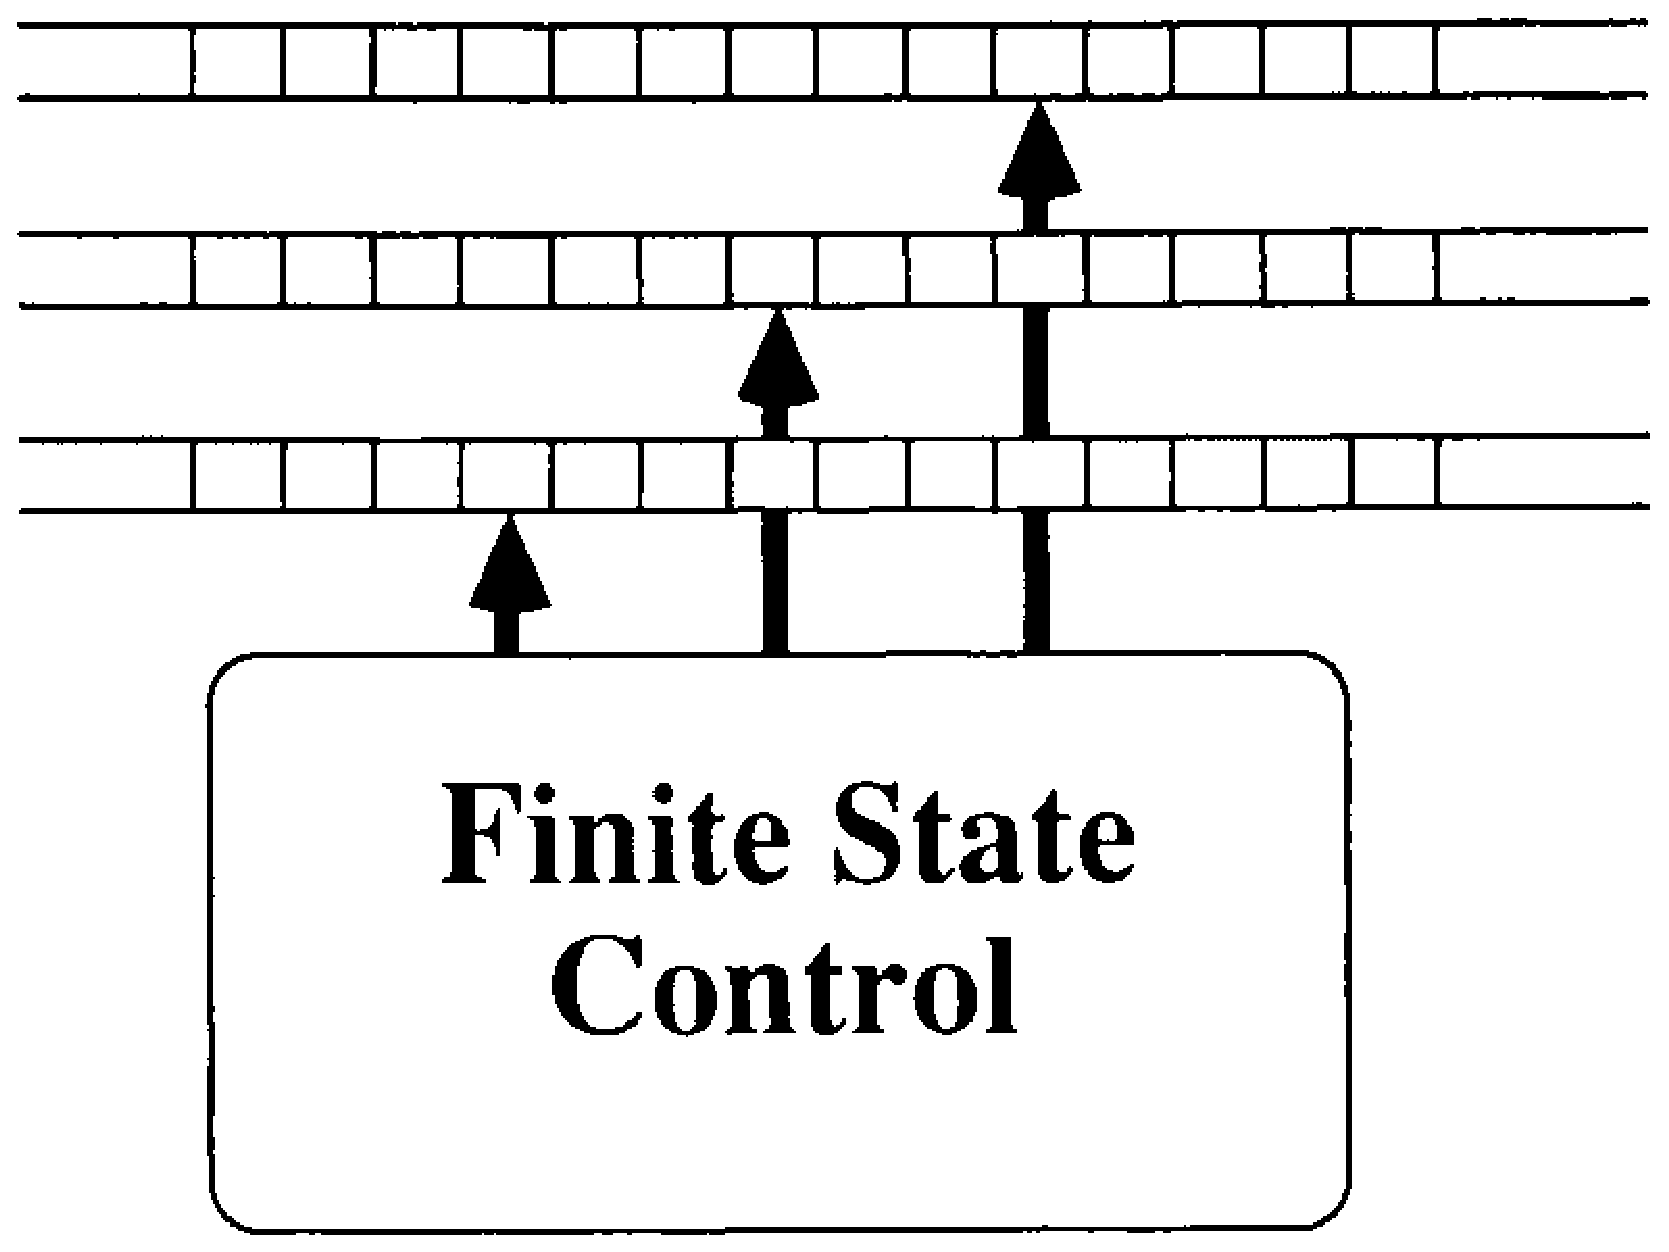
\epsfig{figure=ToFAfigures/fig11-9.eps,width=3.4in}}
\caption{A three-tape Turing machine}\label{fig-11.9}
\end{figure}

% Figure 11.10
\begin{figure}
\centerline{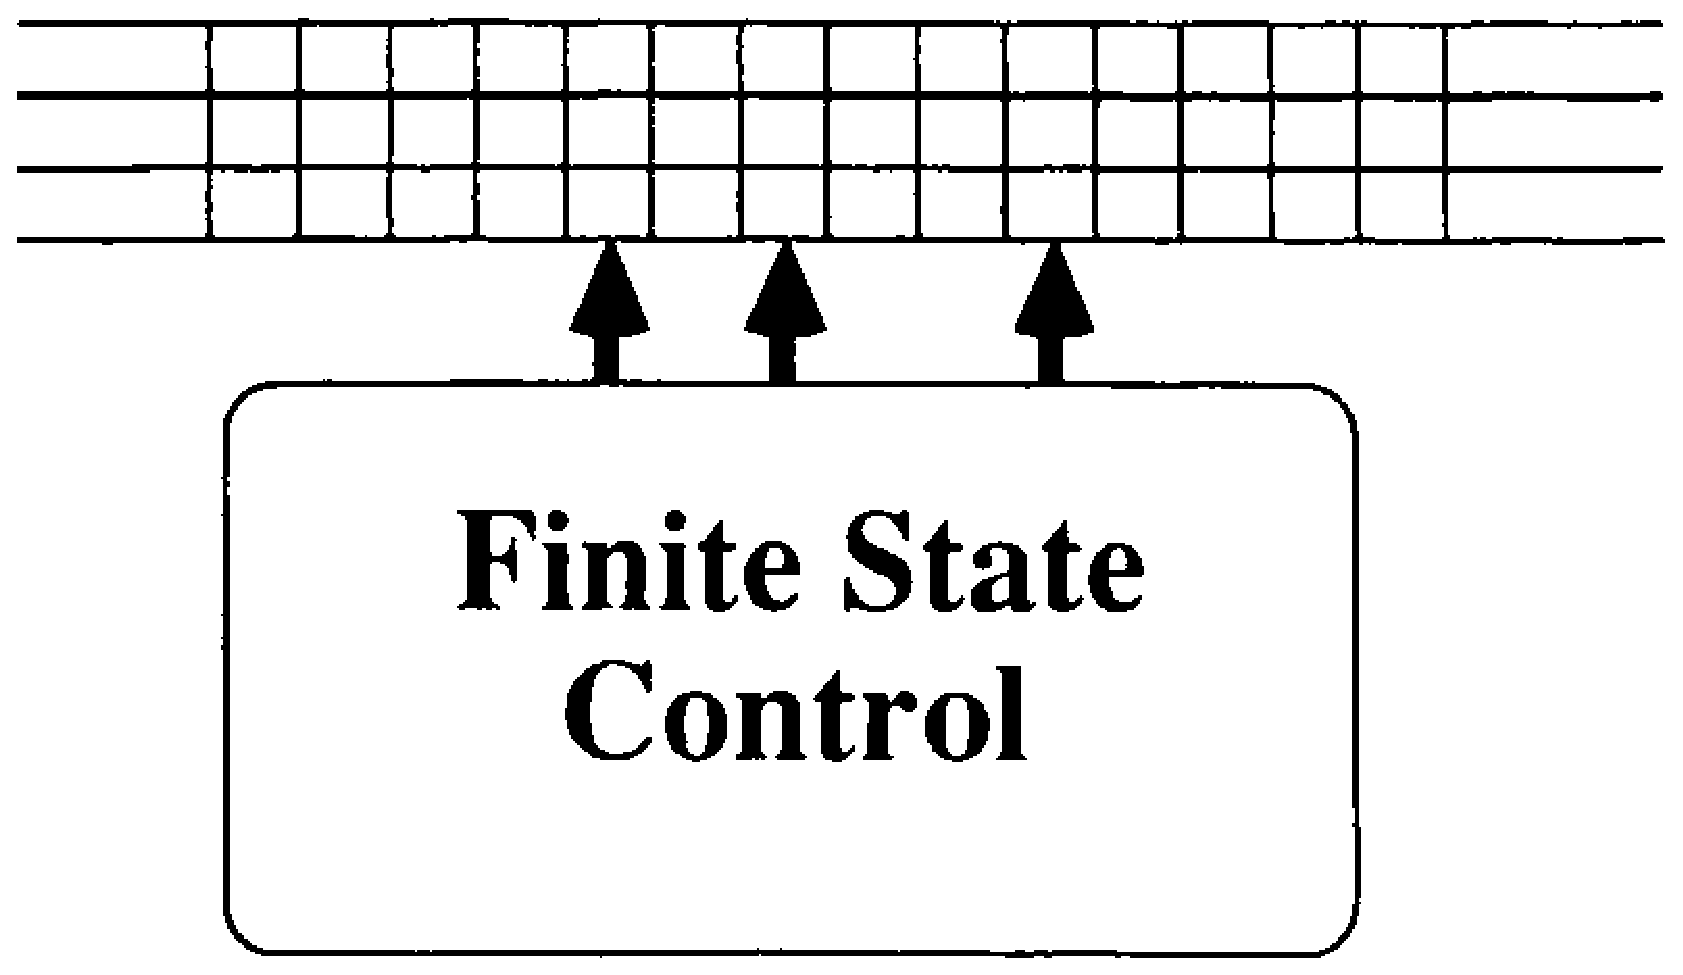
\epsfig{figure=ToFAfigures/fig11-10.eps,width=3.4in}}
\caption{Emulating a three-tape Turing machine with a single three-track tape}\label{fig-11.10}
\end{figure}

One of the wilder enhancements involves the use of a two-dimensional tape, which\index{Turing machine!two-dimensional}
would actually be a surface on which the tape head can move not only left and
right, but also up and down to adjacent squares. With some frantic movement of
the tape head on a one-dimensional tape, two-dimensional Turing machines can be
successfully simulated. Indeed, $k$-dimensional machines (for finite $k$) are no
more powerful than a standard Turing machine. The interested reader is referred
to [HOPC].

\subsection*{Example 11.8}
\index{Turing machine!nondeterministic}
\index{nondeterministic Turing machine}
A potentially more interesting question involves the effects that nondeterminism
might have on the computational power of a Turing machine. With finite automata,
it was seen that NDFAs recognized exactly the same class of languages as DFAs.
However, deterministic pushdown automata accepted a distinctly smaller class of
languages than their nondeterministic cousins. It is consequently hard to
develop even an intuition for what ``should'' happen when nondeterminism is
introduced to the Turing machine construct.

Before we can address this question, we must first define what we mean by a
nondeterministic Turing machine. As with finite automata and pushdown automata,
we may wish to allow a choice of moves from a given configuration, leading to
several disparate sequences of moves for a given input string. Like NDFAs and
NPDAs, we will consider a word accepted if there is at least one sequence of
moves that would have resulted in a $\pmb{Y}$ being printed. Simulating such
machines with deterministic Turing machines is more involved than it may at
first seem. If each possible computation was guaranteed to halt, it would be
reasonable to try each sequence of moves, one after the other, halting only when
a $\pmb{Y}$ was found. If one sequence led to an $\pmb{N}$ being printed, we
would then move on to the next candidate. Since there may be a countable number
of sequences to try, this process may never end. This is not really a problem,
since if a sequence resulting in a $\pmb{Y}$ exists, it will eventually be found
and tried, and the machine will halt and accept the word. If no such sequence
resulting in a $\pmb{Y}$ exists, and there are an infinite number of negative
attempts to be checked, the machine will never halt. By our original definition
of acceptance, this will result in the word being rejected, which is the desired
result.

The trouble arises in trying to simulate machines that are not guaranteed to
halt under all possible circumstances. This is not an inconsequential concern;
in Chapter \ref{ch-12}, we will identify some languages that are so complex that their
corresponding Turing machines cannot halt for all input strings. A problem then
arises in trying to switch from one sequence to the next. If, say, the first
sequence we tried did not halt and instead simply continued operation without
ever producing $\pmb{Y}$ or $\pmb{N}$, we would never get the chance to try
other possible move sequences. Since the machine will not halt, the word will
therefore be rejected, even if some later sequence would have produced
$\pmb{Y}$. Simulating the nondeterministic machine in this manner will not be
guaranteed to recognize the same language, and an alternative method must be
used.

This problem is avoided by simulating the various computations in the following
(very inefficient) manner. We begin by simulating the first move of the first
sequence. We then start over with the first move of the second sequence, and
then begin again and simulate two moves in the first sequence. On the next pass,
we simulate the first move of the third sequence, then two moves of the second
sequence, and then three moves of the first sequence. On each pass, we start
computing a new sequence and move a little further along on the sequences that
have already been started. If any of these sequences results in $\pmb{Y}$, we
will eventually simulate enough of that sequence to discover that fact and
accept the word. In this way, we avoid getting trapped in a dead end with no
opportunity to pursue the alternatives.

Implementing the above scheme will produce a deterministic Turing machine that
is equivalent\index{equivalent!Turing machines} to the original nondeterministic machine. It remains to be shown
that the Turing machine can indeed \emph{start over} as necessary, and that the
possible move sequences can be enumerated in a reasonable fashion so that they
can be pursued according to the pattern outlined above. A three-tape
(deterministic) Turing machine will suffice. The first tape will keep an
inviolate copy of the input string, which will be copied onto the second tape
each time a computation begins anew. A specific sequence of steps will be
carried out on this second scratch tape, after which the presence/absence of $\pmb{Y}$
will be determined. The third tape is responsible for keeping track of the
iterations and generating the appropriate sequences to be employed. Enumerating
the sequences is much like the problem of generating words over some alphabet in
lexicographic order (see the exercises). Methods for generating the ``directing
sequences'' can be found in both [LEWI] and [HOPC]. These references also
propose a more efficient approach to the whole simulation, which is based on
keeping track of the sets of possible configurations, much as was done in
%Theorem \ref{thm-4.5} for nondeterministic finite automata.
% NOTE: Theorem 4.5 does NOT exist
Definition \ref{dfn-4.5} for nondeterministic finite automata.

Thus, neither nondeterminism nor any of the enhancements considered above
improved the computational power of these devices. As mentioned previously, no
one has yet been able to find any mechanical enhancement that does yield a
device that can recognize a language that is not Turing acceptable. Attempts at
producing completely different formal systems have fared no better, and there is
little cause to believe that such systems exist. We now turn to characterizing
what appears to be the largest class of algorithmically definable languages. In
the next section, we will see that the Turing-acceptable languages are exactly
the type 0 languages introduced in Chapter \ref{ch-8}.

% Definition 11.4
\begin{dfn}\label{dfn-11.4}\index{T@\TSIG \ (T-sigma )}\index{Z@\ZSIG \ (Z-sigma )}
For a given alphabet $\Sigma$, let \TSIG\ be the collection of all
Turing-acceptable languages, and let \ZSIG\ be the collection of all type 0
languages.
\end{dfn}

The freedom to use several tapes and nondeterminism makes it easier to explore
the capabilities of Turing machines and relate \TSIG\ to the previous classes of
languages encountered. It is now trivial to justify that every PDA can be
simulated by a nondeterministic Turing machine with two tapes. The first tape
will hold the input, which will be scanned by the first tape head, which will
only have to move right or, at worst, remain stationary and reprint the same
character it was scanning. The second tape will function as the stack, with
strings pushed or symbols popped in correspondence with what takes place in the
PDA. Since a Turing machine can only print one symbol at a time, some new states
may be needed in the finite-state control to simulate pushing an entire string,
but the translation process is quite direct.

% Lemma 11.1
\begin{lmm}\label{lmm-11.1}
Let $\Sigma$ be an alphabet. Then $\PSIG\subset\TSIG$. That is, every
context-free language is Turing acceptable, and the containment is proper.

\emph{Proof.} Containment follows from the formalization of the above discussion
(see the exercises). Example 11.3 presented a language over $\{\pmb{a},\pmb{b},
\pmb{c}\}$ that is Turing acceptable but not context free. While the distinction
between \DSIG, and \PSIG, disappeared for singleton alphabets, proper
containment remains between $\mathfrak{P}_{\{\pmb{a}\}}$ and $\mathfrak{T}_{\{
\pmb{a}\}}$, as shown by languages such as $\{\pmb{a}^n|\ n$ is a perfect square
$\}$.
\end{lmm}

In the next section, an even stronger result is discussed, which shows that the
class of Turing-acceptable languages includes much more than just the
context-free languages. Lemma \ref{lmm-11.1} is actually an immediate corollary of Theorem
\ref{thm-11.2}. The next section also explores the formal relationship between Turing
machines and context-sensitive languages.

\section{Turing Machines, LBAs, and Grammars}\label{sec-11.3}

The previous sections have shown that the class of Turing-acceptable languages
properly contains the type 2 languages. We now explore how the type 0 and type
1 languages relate to Turing machines. Since the preceding discussions mentioned
that no formal systems have been found that surpass Turing machines, one would
expect that every language generated by a grammar can be recognized by a Turing
machine. This is indeed the case, as indicated by the following theorem.

% Theorem 11.2
\begin{thm}\label{thm-11.2}\index{equivalent!Turing machines}
Let $\Sigma$ be an alphabet. Then $\ZSIG\subseteq\TSIG$. That is, every type 0
language is Turing acceptable.

\emph{Proof.} We justify that, given any type 0 grammar $G=\langle\Sigma,\Gamma,
S,P\rangle$, there must be a Turing machine $T_G$ that is equivalent to $G$. As
with the suggested conversion of a PDA to a Turing machine, $T_G$ will employ
two tapes and nondeterminism. The first tape again holds the input, which will
be compared to the sentential form generated on the second tape. The second tape
begins with only the start symbol on an otherwise blank tape. The finite-state
control is responsible for nondeterministically guessing the proper sequence of
productions to apply, and with each guess, the second tape is modified to
reflect the new sentential form. If at some point the sentential form agrees
with the contents of the first tape, the machine prints $\pmb{Y}$ and halts. A
guess will consist of choosing both an arbitrary position within the current
sentential form and a particular production to attempt to substitute for the
substring beginning at that position. Only words that can be generated by the
grammar will have a sequence of moves that produces $\pmb{Y}$, and no word that
cannot be generated will be accepted. Thus, the new Turing machine is equivalent
to $G$.
\end{thm}

\subsection*{Example 11.9}

Consider the context-sensitive grammar $G=\langle\{\pmb{a},\pmb{b},\pmb{c}\},\{
S,A,B,C\},S,P\rangle$, where $P$ contains the productions
\begin{enumerate}
\item $Z\rightarrow\lambda$
\vspace{-0.1in}
\item $Z\rightarrow S$
\vspace{-0.1in}
\item $S\rightarrow SABC$
\vspace{-0.1in}
\item $S\rightarrow ABC$
\vspace{-0.1in}
\item $AB\rightarrow BA$
\vspace{-0.1in}
\item $BA\rightarrow AB$
\vspace{-0.1in}
\item $CB\rightarrow BC$
\vspace{-0.1in}
\item $BC\rightarrow CB$
\vspace{-0.1in}
\item $CA\rightarrow AC$
\vspace{-0.1in}
\item $AC\rightarrow CA$
\vspace{-0.1in}
\item $A\rightarrow\pmb{a}$
\vspace{-0.1in}
\item $B\rightarrow\pmb{b}$
\vspace{-0.1in}
\item $C\rightarrow\pmb{c}$
\end{enumerate}
It is quite easy to show that $L(G)=\{x\in\{\pmb{a},\pmb{b},\pmb{c}\}^*|\ \
|x|_{\pmb{a}}=|x|_{\pmb{b}}=|x|_{\pmb{c}}\}$ by observing that no production
changes the relative numbers of (lowercase and capital) $A$s, $B$s, and $C$s,
and the six context-sensitive rules allow them to be arbitrarily reordered. One
of the attempted ``guesses'' made by the Turing machine $T_G$ concerning how the
productions might be applied is:
\begin{quote}
Use (2) beginning at position 1. \\
Use (4) beginning at position 1. \\
Use (6) beginning at position 2. $\ldots$
\end{quote}
This would lead to a failed attempt, since it corresponds to $Z\Rightarrow S
\Rightarrow ABC$, and the substring $BC$ beginning at position 2 does not match
$BA$, the left side of rule 6. On the other hand, there is a pattern of guesses
that would cause the following sequence of symbols to appear on the second tape:
\[ Z\Rightarrow S\Rightarrow ABC\Rightarrow BAC\Rightarrow BCA\Rightarrow
	B\pmb{c}A\Rightarrow B\pmb{ca}\Rightarrow\pmb{bca} \]
This would lead to a favorable comparison if $\pmb{bca}$ was the word on the
input tape. Note that the Turing machine may have to handle shifting over
existing symbols on the scratch tape to accommodate increases in the size of the
sentential form. Since type 0 grammars allow length-reducing productions, the
machine may also be required to shrink the sentential form when a string of
symbols is replaced by a smaller string.

A rather nice feature of type 1 languages is that the length of the sentential
form could never decrease (except perhaps for the application of the initial
production $Z\rightarrow\lambda$), and hence sentential forms that become
longer than the desired word are known to be hopeless. All context-sensitive
(that is, type 1) languages can therefore be recognized by a Turing machine that
use an amount of tape proportional to the length of the input string, as
outlined below.

% Definition 11.5
\begin{dfn}\label{dfn-11.5}\index{alphabet!input}\index{alphabet!auxiliary}
A \emph{\Index{linear bounded automaton}} (\Index{LBA})\index{Turing machine!bounded|see{LBA}}\index{Turing machine!linear bounded|see{LBA}} is a nondeterministic\index{state transition function!for LBA}
Turing machine that recognizes words over an alphabet $\Sigma$ given by the
quintuple $M=\langle\Sigma,\Gamma,S,s_0,\delta\rangle$, where
\begin{quote}
$\Sigma$ is the \emph{input alphabet} \\
$\Gamma$ is the \emph{auxiliary alphabet} containing the special markers $\<$ and\index{end markers for LBA}
	$\>$ and $\Sigma$, $\Gamma$, and $\{\pmb{L},\pmb{R}\}$ are pairwise
	disjoint sets (and thus $\<,\> \notin\Sigma$). \\
$S$ is a finite nonempty set of \emph{states} (and $S\cap(\Sigma\cup\Gamma) =
	\emptyset$). \\
$s_0$ is the \emph{\Index{start state}} ($s_0\in S$). \\
$\delta$ is the \emph{state transition function} $\delta$: $S\times(\Sigma\cup
	\Gamma)\rightarrow(S\cup\{h\}\times(\Sigma\cup\Gamma\cup\{\pmb{L},
	\pmb{R}\})$, where \\
$(\forall s\in S)(\delta(s,\<)=(q,\pmb{R})$ for some $q\in S\cup\{h\})$, and \\
$(\forall s\in S)(\delta(s,\>)=(q,\pmb{L})$ for some $q\in S\cup\{h\}$, or
$\delta(s,\>)=(h,\pmb{Y})$ or $\delta(s,\>)=\langle h,\pmb{N}\rangle)$
\end{quote}
\end{dfn}
That is, the automaton cannot move left of the symbol $\<$ nor overwrite it. The
LBA likewise cannot move right of the symbol $\>$, and it can only overwrite it
with $\pmb{Y}$ or $\pmb{N}$ just prior to halting. The symbols $\#,\pmb{L},\ 
\pmb{R},\ \pmb{Y}$, and $\pmb{N}$ retain their former meaning, although $\#$ can
be dropped from $\Gamma$ since it will never be scanned. As implied by the
following definition, the special markers $\<$ and $\>$ are intended to delimit
the input string, and Definition \ref{dfn-11.5} ensures that the automaton cannot move
past these limits. As has been seen, the use of several tracks can easily
multiply the amount of information that can be stored in a fixed amount of
space, and thus the restriction is essentially that the amount of available tape
is a linear function of the length of the input string. In practice, any Turing
machine variant for which each tape head is constrained to operate within an
area that is a multiple of the length of the input string is called a linear
bounded automaton.

% Definition 11.6
\begin{dfn}\label{dfn-11.6}
For a linear bounded automaton $M=\langle\Sigma,\Gamma,S,s_0,\delta\rangle$, the
\emph{\Index{language accepted by M}}, denoted by $L(M)$, is $L(M)=\{x\in
\Sigma^*|\ \<s_0x\>\Dvdash \<xh\pmb{Y}\}$. A language accepted by a linear bounded
automaton is called a \emph{linear bounded language} (\Index{LBL}).\index{linear bounded language|see{LBL}}\index{language!linear bounded}
\end{dfn}

Note that while the endmarkers must enclose the string $x$, it is the word $x$
(rather than $\<x\>$) that is considered to belong to $L(M)$. As before, other
criteria for acceptance are equivalent to Definition \ref{dfn-11.6}. The set of all words
for which a LBA merely halts can be shown to be a LBL according to the above
definition. The following example illustrates a linear bounded automaton that is
intended to recognize all words that cause the machine to print $\pmb{Y}$ at the
end of the (obliterated) word. Example 11.13 illustrates a general technique for
restoring the input word, producing an LBA that accepts according to Definition
\ref{dfn-11.6}.

\subsection*{Example 11.10}

Consider the machine $L$ shown in Figure \ref{fig-11.11} and the input string
$\pmb{babcca}$. The following steps show that $\<s_0\pmb{babcca}\>\Dvdash
\<\pmb{XXXXXXhY}$.
\begin{center}\begin{tabular}{r@{ }l@{ }l@{ }l@{ }l}
$\<s_0\pmb{babcca}\>$ & $\vdash \<\pmb{b}s_1\pmb{abcca}\>$ & $\vdash \<\pmb{b}s_2
	\pmb{Xbcca}\>$ & $\vdash \<s_2\pmb{bXbcca}\>$ & $\vdash$ \\
$s_2\<\pmb{bXbcca}\>$ & $\vdash \<s_3\pmb{bXbcca}\>$ & $\vdash \<s_4\pmb{XXbcca}\>$ &
	$\vdash s_4\<\pmb{XXbcca}\>$ & $\vdash$ \\
$\<s_5\pmb{XXbcca}\>$ & $\vdash \<\pmb{X}s_5\pmb{Xbcca}\>$ & $\vdash \<\pmb{XX}s_5
	\pmb{bcca}\>$ & $\vdash \<\pmb{XXb}s_5\pmb{cca}\>$ & $\vdash$ \\
$\<\pmb{XXb}s_6\pmb{Xca}\>$ & $\vdash \<\pmb{XX}s_6\pmb{bXca}\>$ & $\vdash \<\pmb{X}
	s_6\pmb{XbXca}\>$ & $\vdash \<s_6\pmb{XXbXca}\>$ & $\vdash$ \\
$s_6\<\pmb{XXbXca}\>$ & $\vdash \<s_0\pmb{XXbXca}\>$ & $\vdash \<\pmb{X}s_0
	\pmb{XbXca}\>$ & $\vdash \<\pmb{XX}s_0\pmb{bXca}\>$ & $\vdash$ \\
$\<\pmb{XXb}s_1\pmb{Xca}\>$ && $\Dvdash s_2\<\pmb{XXbXcX}\>$ && $\Dvdash$ \\
$\<\pmb{XX}s_3\pmb{bXcX}\>$ && $\Dvdash s_4\<\pmb{XXXXcX}\>$ && $\Dvdash$ \\
$\<\pmb{XXXX}s_5\pmb{cX}\>$ && $\Dvdash s_6\<\pmb{XXXXXX}\>$ && $\Dvdash$ \\
$\<\pmb{XXXXXX}s_0\>$ && $\vdash \<\pmb{XXXXXXhY}$
\end{tabular}\end{center}

% Figure 11.11
\begin{figure}
\centerline{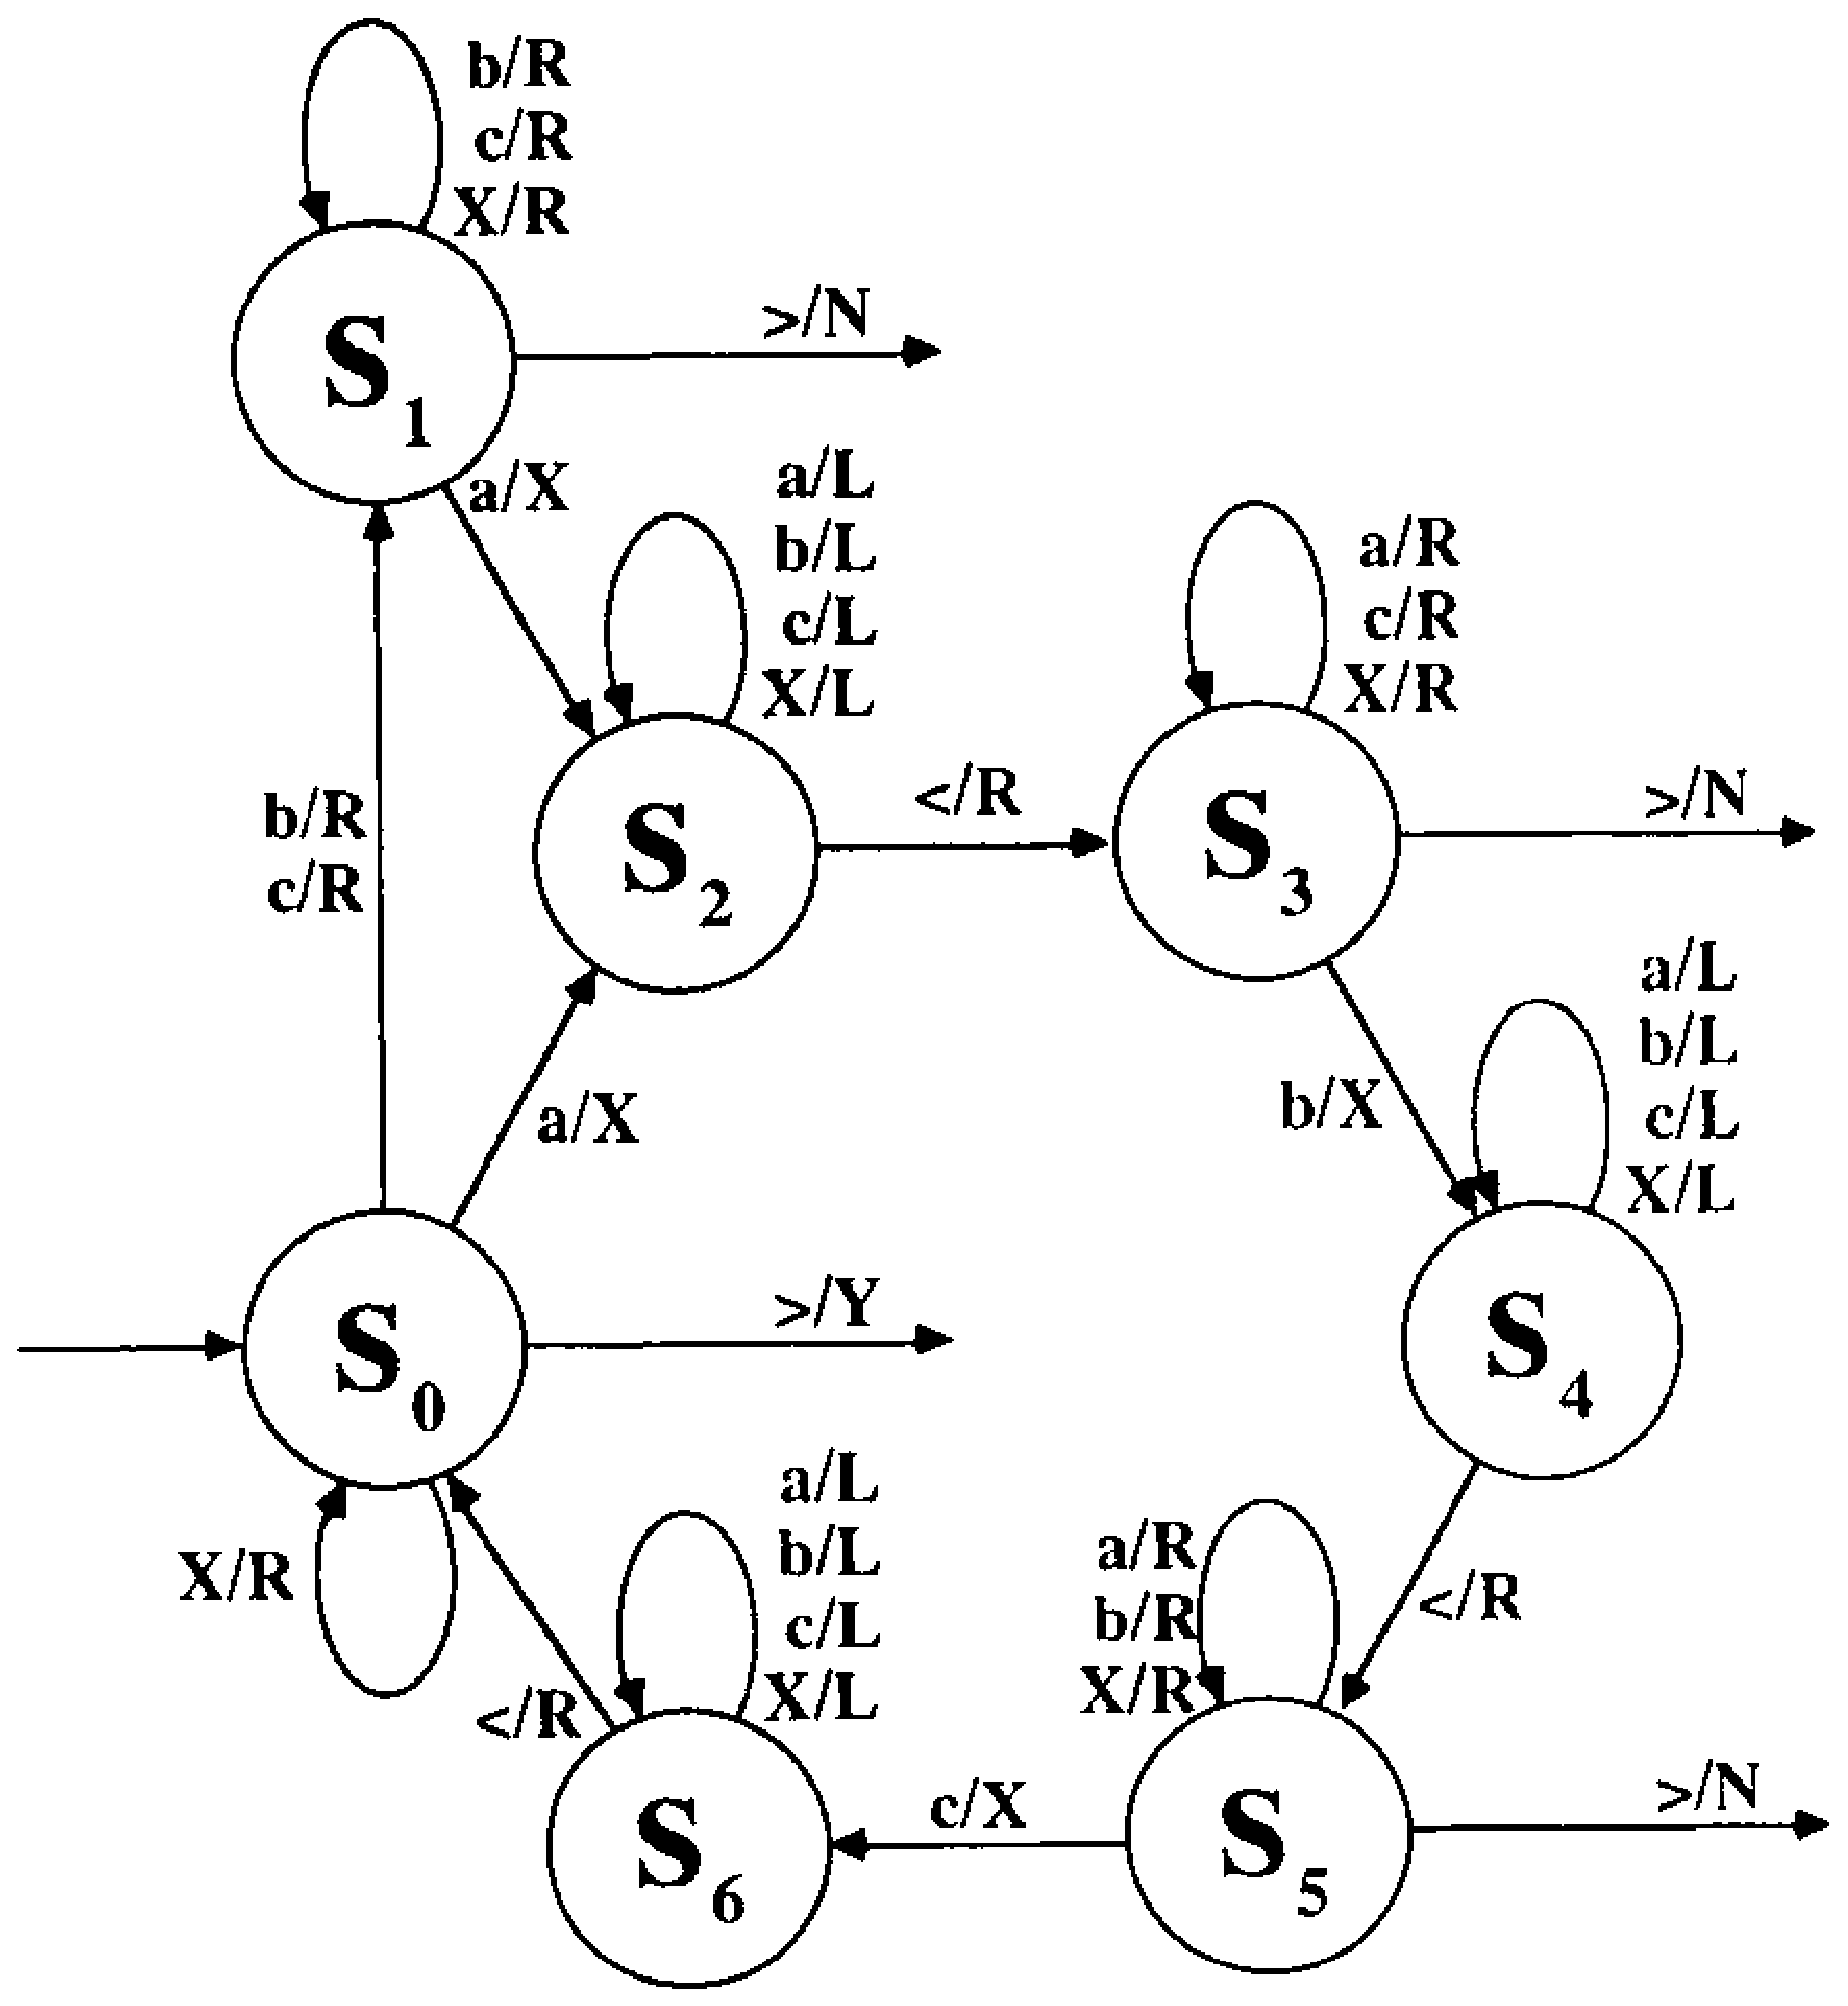
\epsfig{figure=ToFAfigures/fig11-11.eps,width=3.4in}}
\caption{The Turing machine discussed in Example 11.10}\label{fig-11.11}
\end{figure}

% Definition 11.7
\begin{dfn}\label{dfn-11.7}\index{O@\OSIG \ (O-sigma )}\index{L@\LSIG \ (L-sigma )}
For a given alphabet $\Sigma$, let \LSIG\ be the collection of all linear
bounded languages, and let \OSIG\ be the collection of all context-sensitive
(type 1) languages.
\end{dfn}

The proof of Theorem \ref{thm-11.2} can be modified to show that all context-sensitive
languages can be recognized by linear bounded automata. Since context-sensitive
languages do not contain contracting productions, no sentential forms that are
longer than the desired word need be considered. Consequently, the two-tape
Turing machine in Theorem \ref{thm-11.2} can operate as a linear bounded automaton. The
first tape with the input word never changes and thus satisfies the boundary
restriction, while the finite-state control can simply abort any computation on
the second tape that violates the length restriction. Just as Theorem \ref{thm-11.2}
showed that $\ZSIG\subseteq\TSIG$ we now have a relationship between another
pair of cognitive and generative classes.

% Theorem 11.3
\begin{thm}\label{thm-11.3}\index{equivalent!Turing machines}
Let $\Sigma$ be an alphabet. Then $\OSIG\subseteq\LSIG$. That is, every type
1 language is a LBL.

\emph{Proof.} The proof follows from the formalization of the above discussion
(see the exercises).
\end{thm}

We have argued that every type 0 grammar must have an equivalent Turing machine,
and it can conversely be shown that every Turing-acceptable language can be
generated by a type 0 grammar. To do this, it is most convenient to use the very
restrictive criteria for a Turing-acceptable language given in Definition \ref{dfn-11.3},
in which the original input string is not destroyed. For Turing machines which
behave in this fashion, the descriptions of the device configurations bear a
remarkable resemblance to the derivations in a grammar.

\subsection*{Example 11.11}

% Figure 11.12
\begin{figure}
\centerline{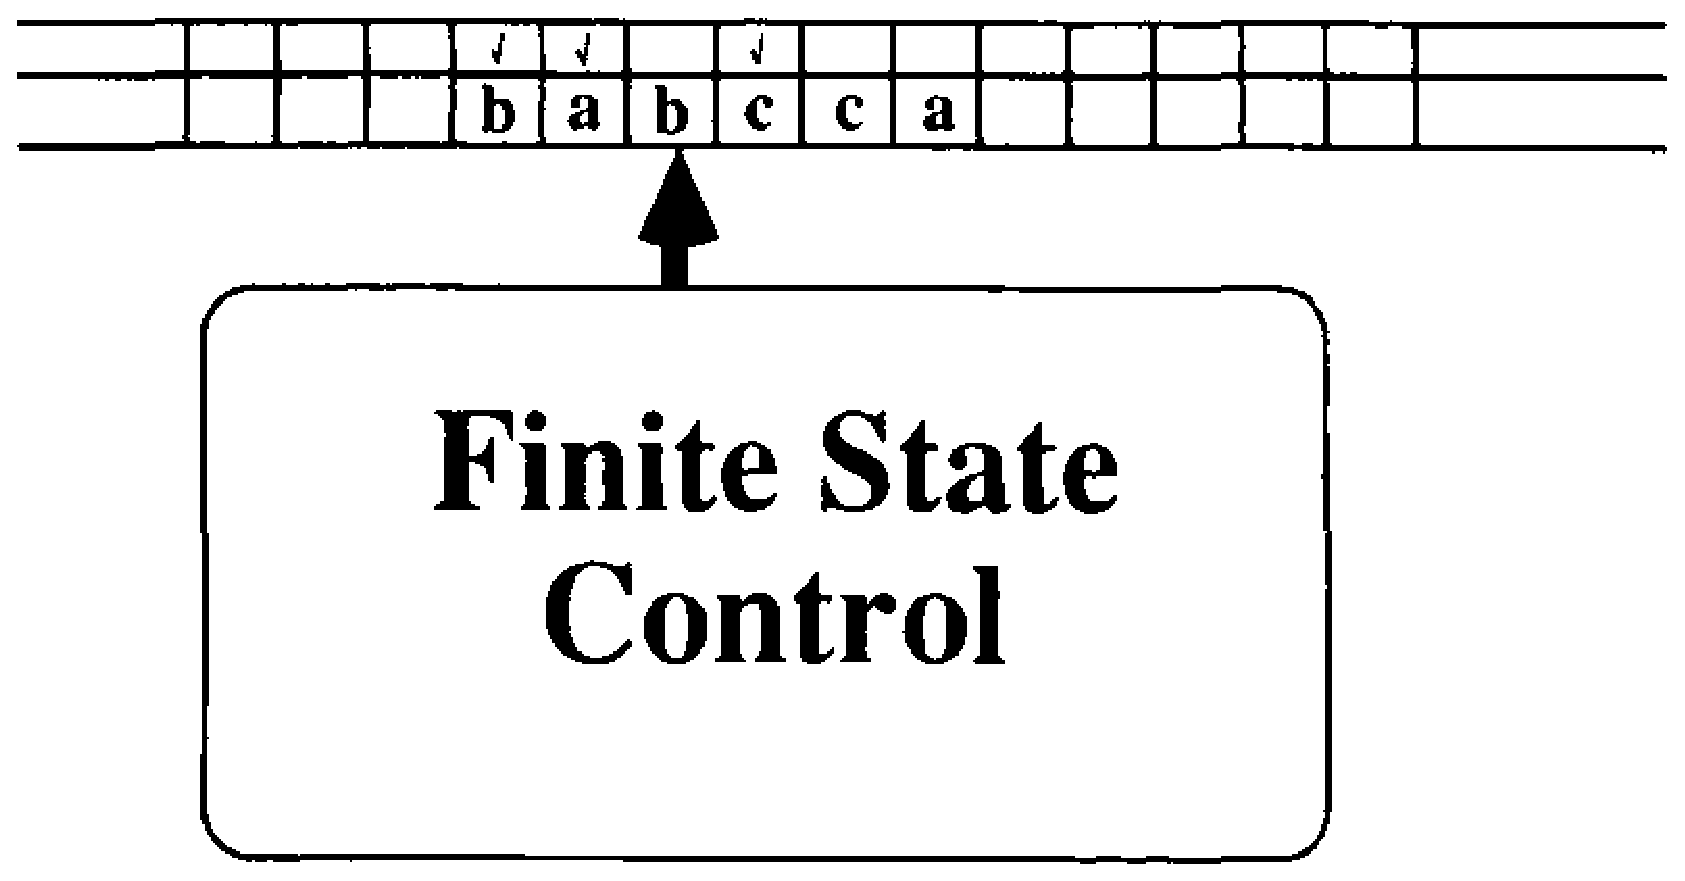
\epsfig{figure=ToFAfigures/fig11-12.eps,width=3.4in}}
\caption{The Turing machine discussed in Example 11.11}\label{fig-11.12}
\end{figure}

Consider again the language $\{x\in\{\pmb{a},\pmb{b},\pmb{c}\}^*|\ \ |x|_{\pmb{a}}
=|x|_{\pmb{b}}=|x|_{\pmb{c}}\}$. As discussed in Example 11.3, the Turing machine
in Figure \ref{fig-11.4} destroys the word originally on the input tape. Figure \ref{fig-11.12}
depicts a slightly more complex Turing machine that restores the original word
just prior to acceptance. It will (fortunately) not generally be necessary for
our purposes to restore rejected words, since there are intricate languages for
which this is not always possible. The modified quintuple is $T=\langle\{\pmb{a},
\pmb{b},\pmb{c}\},\{\pmb{\#},\pmb{A},\pmb{B},\pmb{C},\pmb{Y},\pmb{N}\},\{s_0,s_1,
s_2,s_3,s_4,\\s_5,s_6,s_7,s_8\},s_0,\delta\rangle$, where $\delta$ is as indicated
in the diagram in Figure \ref{fig-11.13}. ``Saving'' the original input string is
accomplished by replacing occurrences of the different letters by distinct
symbols and restoring them later. The implementation reflects one of the first
uses suggested for multiple-track machines: using the second track to check off
input symbols. For legibility, an $\pmb{a}$ with a check mark above it is denoted by
$\pmb{A}$, while an $\pmb{a}$ with no check mark remains an $\pmb{a}$. Similarly,
checked $\pmb{b}$s are represented by $\pmb{B}$ and checked $\pmb{c}$s by
$\pmb{C}$. Thus, if the string $\pmb{BAbCca}$ were on a two-track tape employing
check marks, it would look like
% Get better check symbol than sqrt
\begin{center}\begin{tabular}{ll}
$\!\surd\!\!\surd\ \ \surd$ \\
$\pmb{babcca}$
\end{tabular}\end{center}
The additional states $s_7$ and $s_8$ essentially erase the check marks just
before halting by replacing $\pmb{A}$ with $\pmb{a}$, $\pmb{B}$ with $\pmb{b}$,
and $\pmb{C}$ with $\pmb{c}$.

% Figure 11.13
\begin{figure}
\centerline{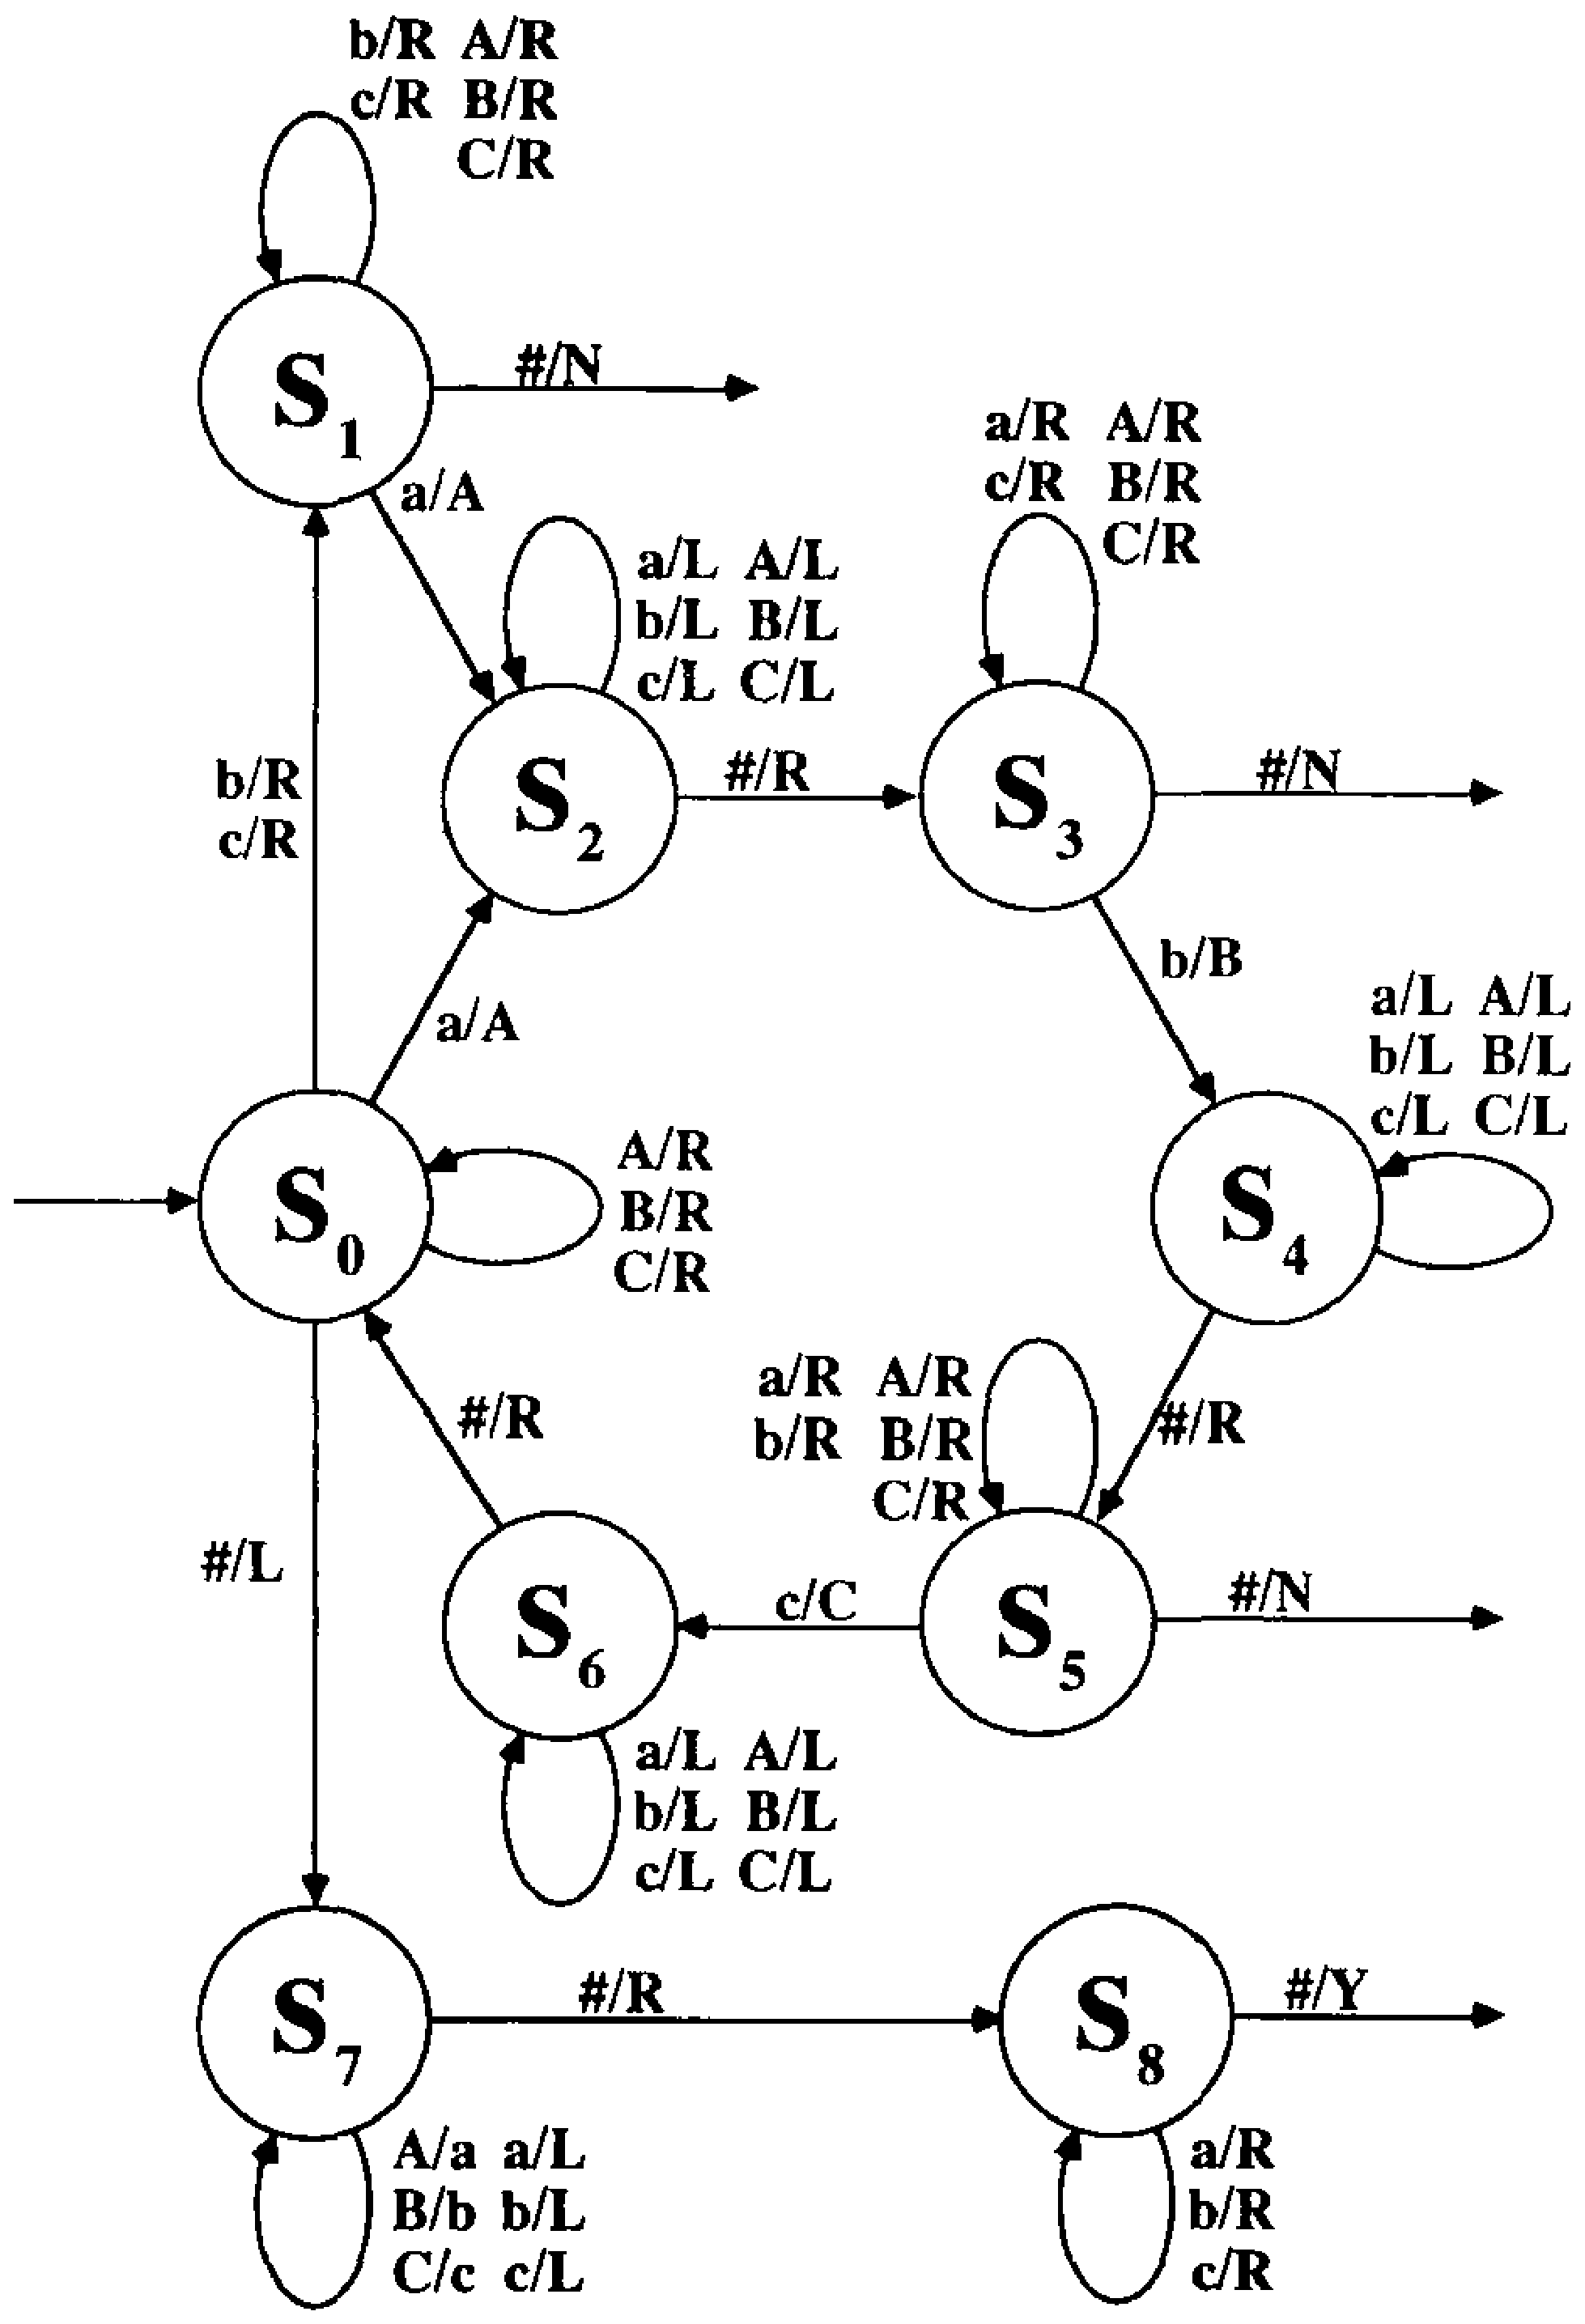
\epsfig{figure=ToFAfigures/fig11-13.eps,height=3.8in}}
\caption{The state transition diagram discussed in Example 11.11}\label{fig-11.13}
\end{figure}

Consider again the input string $\pmb{babcca}$ processed by the Turing machine
in Example 11.3. It is also accepted by this Turing machine because the
following steps show that $s_0\pmb{babcca}\Dvdash\pmb{babccahY}$. Note how
closely the steps correspond with those in Example 11.3. The sequence below also
illustrates how $s_7$ converts the string back to lowercase, after which $s_8$
returns the tape head to the right for acceptance.

\begin{center}\begin{tabular}{r@{ }l@{ }l@{ }l@{ }l@{ }}
$s_0\pmb{babcca}$ & $\vdash\pmb{b}s_1\pmb{abcca}$ & $\vdash\pmb{b}s_2\pmb{Abcca}$
	& $\vdash s_2\pmb{bAbcca}$ & $\vdash$ \\
$s_2\pmb{\#bAbcca}$ & $\vdash s_3\pmb{bAbcca}$ & $\vdash s_4\pmb{BAbcca}$ &
	$\vdash s_4\pmb{\#BAbcca}$ & $\vdash$ \\
$s_5\pmb{BAbcca}$ & $\vdash\pmb{B}s_5\pmb{Abcca}$ & $\vdash\pmb{BA}s_5
	\pmb{bcca}$ & $\vdash\pmb{BAb}s_5\pmb{cca}$ & $\vdash$ \\
$\pmb{BAb}s_6\pmb{Cca}$ & $\vdash\pmb{BA}s_6\pmb{bCca}$ & $\vdash\pmb{B}s_6
	\pmb{AbCca}$ & $\vdash s_6\pmb{BAbCca}$ & $\vdash$ \\
$s_6\pmb{\#BAbCca}$ & $\vdash s_0\pmb{BAbCca}$ &
$\vdash\pmb{B}s_0\pmb{AbCca}$ &
	$\vdash\pmb{BA}s_0\pmb{bCca}$ & $\vdash$ \\
$\pmb{BAb}s_1\pmb{Cca}$ && $\Dvdash s_2\pmb{\#BAbCcA}$ && $\Dvdash$ \\
$\pmb{BA}s_3\pmb{bCca}$ && $\Dvdash s_4\pmb{\#BABCcA}$ && $\Dvdash$ \\
$\pmb{BABC}s_5\pmb{cA}$ && $\Dvdash s_6\pmb{\#BABCCA}$ && $\Dvdash$ \\
$\pmb{BABCCA}s_0$ & $\vdash\pmb{BABCC}s_7\pmb{A}$ & $\vdash\pmb{BABCC}s_7
	\pmb{a}$ & $\vdash\pmb{BABC}s_7\pmb{Ca}$ & $\vdash$ \\
$\pmb{BABC}s_7\pmb{ca}$ && $\Dvdash s_7\pmb{babcca}$ & $\vdash
s_7\pmb{\#babcca}$
	& $\vdash$ \\
$s_8\pmb{babcca}$ & $\vdash\pmb{b}s_8\pmb{abcca}$ & $\Dvdash\pmb{babcca}s_8$
&&
	$\vdash$ \\
$\pmb{babccahY}$
\end{tabular}\end{center}

If occurrences of the machine transition symbol $\vdash$ are replaced by the
derivation symbol $\Rightarrow$, the above sequence would look remarkably like a
derivation in a type 0 grammar. Indeed, we would like to construct a grammar in
which sentential forms like $\pmb{b}s_1\pmb{abcca}$ could be derived from
$s_0\pmb{babcca}$ in one step. Since the machine changed configurations because
of the transition rule $\delta(s_0,\pmb{b})=\langle s_1,\pmb{R}\rangle$, this
transition should have a corresponding production of the form $s_0\pmb{b}
\rightarrow\pmb{b}s_1$. Each transition in the Turing machine will be
responsible for similar productions.

Unfortunately, the correspondence between transition rules and productions is
complicated by the fact that the tape head may occasionally scan blank cells,
which must then be added to the sentential form. The special characters `$[$' and
`$]$' will bracket the sentential form throughout this stage of the derivation and
will indicate the current left and right limits of the tape head travel,
respectively. Attempting to move left past the conceptual position of `$[$' (or
right past the position of `$]$'\,) will result in the addition of a blank symbol to
the sentential form.

To generate the words accepted by a Turing machine, our grammar will randomly
generate a word over $\Sigma$, delimit it by brackets, and insert the symbol for
the start state at the left edge. The rules derived from the transitions should
then be able to transform a string such as $[s_0\pmb{babcca\#}]$ into
$[\pmb{\#babccahY\#}]$. Since only the letters in $\Sigma$ will be considered
terminal symbols, the symbols $[$, $]$, $\pmb{\#}$, and $\pmb{Y}$ are
nonterminals, and the derivation will not yet be complete. To derive terminal
strings for just the accepted words, the presence of $\pmb{Y}$ will allow
further productions to delete those remaining nonterminals.

% Definition 11.8
\begin{dfn}\label{dfn-11.8}\index{Turing machine!corresponding grammar}
Given a Turing machine $M=\langle\Sigma,\Gamma,S,s_0,\delta\rangle$, the grammar
corresponding to $M$, $G_M$, is given by $G_M=\langle\Sigma,\Gamma\cup S\cup\{Z,
W,U,V,[,]\},Z,P_M\rangle$, where $P_M$ contains the following classes of
productions:
\begin{enumerate}
\item $Z\rightarrow[W\pmb{\#}]\in P_M$ \\
$(\forall \pmb{a}\in\Sigma)([W\rightarrow[W\pmb{a}\in P_M)$ \\
$W\rightarrow s_0\in P_M$

\item Each printing transition gives rise to a production rule as follows
\[ (\forall s\in S)(\forall t\in S\cup\{h\})(\forall\pmb{a},\pmb{b}\in\Sigma\cup
	\Gamma)(\text{if }\delta(s,\pmb{a})=\langle t,\pmb{b}\rangle,
	\text{ then }s\pmb{a}\rightarrow t\pmb{b}\in P_M) \]
Each move right gives rise to a production rule as follows
\[ (\forall s,t\in S)(\forall\pmb{a}\in\Sigma\cup\Gamma)(\text{if }\delta(s,
	\pmb{a})=\langle t,\pmb{R}\rangle,\text{ then }s\pmb{a}\rightarrow
	\pmb{a}t\in P_M) \]
If $\pmb{a}=\pmb{\#}$, an additional production is needed:
\[ (\forall s,t\in S)(\text{if }\delta(s,\pmb{\#})=\langle t,\pmb{R}\rangle,
	\text{ then }s]\rightarrow\pmb{\#}t]\in P_M) \]
Each move left gives rise to a production rule as follows
\begin{center}\begin{tabular}{l}
$(\forall s,t\in S)(\forall\pmb{a}\in\Sigma\cup\Gamma)$ \\
$(\text{if }\delta(s,\pmb{a})=\langle t,\pmb{L}\rangle,\text{ then }[s\pmb{a}
	\rightarrow [t\pmb{\#a}\in P_M\wedge (\forall\pmb{d}\in\Sigma\cup\Gamma)
	(\pmb{d}s\pmb{a}\rightarrow t\pmb{da}\in P_M))$
\end{tabular}\end{center}

\item $h\pmb{Y}\rightarrow U\in P_M$ \\
$U\pmb{\#}\rightarrow U\in P_M$ \\
$U]\rightarrow V\in P_M$ \\
$(\forall\pmb{a}\in\Sigma)(\pmb{a}V\rightarrow V\pmb{a}\in P_M)$ \\
$\pmb{\#}V\rightarrow V\in P_M$ \\
$[V\rightarrow \lambda\in P_M$
\end{enumerate}
\end{dfn}

The rules in class 1 are intended to generate all words of the form $[s_0x
\pmb{\#}]$, where $x$ is an arbitrary member of $\Sigma^*$. The remaining rules
are defined in such a way that only those strings $x$ that are recognized by $M$
can successfully produce a terminal string. Note that once $W$ is replaced by
$s_0$, neither $Z$ nor $W$ can appear in a later sentential form. After $s_0$ is
generated, the rules in class 2 may apply. It can be inductively argued that the
derivations arising from the application of these rules directly reflect the
changes in the configuration of the Turing machine (see Theorem \ref{thm-11.4}).

None of the class 3 productions can be used until the point at which the halt
state would be reached in the corresponding computation. Since $h\notin S$, none
of the class 2 productions can then be used. Only if $\pmb{Y}$ was written to tape as
the Turing machine halted will the production $h\pmb{Y}\rightarrow U$ be
applicable. $U$ will then delete the trailing blanks and $]$ from the sentential
form, and then $V$ will percolate to the left, removing the leading blanks and
the final nonterminal $[$, leaving only the terminal string $x$ in the
(completed) sentential form. The following example illustrates a derivation
stemming from a typical Turing machine.

\subsection*{Example 11.12}

Consider the Turing machine $T$ in Figure \ref{fig-11.13} and the corresponding grammar
$G_T$. Among the many possible derivations involving the class 1 productions is
\begin{center}\begin{tabular}{r@{ $\Rightarrow$ }l}
$Z$ & $[W\pmb{\#}]\Rightarrow[W\pmb{a\#}]\Rightarrow[W\pmb{ca\#}]\Rightarrow
	[W\pmb{cca\#}]\Rightarrow[W\pmb{bcca\#}]\Rightarrow[W\pmb{abcca\#}]$ \\
& $[W\pmb{babcca\#}]\Rightarrow[s_0\pmb{babcca\#}]$
\end{tabular}\end{center}
Only class 2 productions apply at this point, and there is exactly one
derivation applicable at each step in the following sequence.
\begin{center}\begin{tabular}{r@{ }l@{ }l@{ }l@{ }l}
$[s_0\pmb{babcca\#}]$ & $\Rightarrow[\pmb{b}s_1\pmb{abcca\#}]$ & $\Rightarrow
	[\pmb{b}s_2\pmb{Abcca\#}]$ & $\Rightarrow[s_2\pmb{bAbcca\#}]$ &
	$\Rightarrow$ \\
$[s_2\pmb{\#bAbcca\#}]$ & $\Rightarrow[\pmb{\#}s_3\pmb{bAbcca\#}]$ &
	$\Rightarrow[\pmb{\#}s_4\pmb{BAbcca\#}]$ & $\Rightarrow[s_4\pmb{\#BAbcca
	\#}]$ & $\Rightarrow$ \\
$[\pmb{\#}s_5\pmb{BAbcca\#}]$ & $\Rightarrow[\pmb{\#B}s_5\pmb{Abcca\#}]$ &
	$\Rightarrow[\pmb{\#BA}s_5\pmb{bcca\#}]$ & $\Rightarrow[\pmb{\#BAb}s_5
	\pmb{cca\#}]$ & $\Rightarrow$ \\
$[\pmb{\#BAb}s_6\pmb{Cca\#}]$ & $\Rightarrow[\pmb{\#BA}s_6\pmb{bCca\#}]$ & 
	$\Rightarrow[\pmb{\#B}s_6\pmb{AbCca\#}]$ & $\Rightarrow[\pmb{\#}s_6
	\pmb{BAbCca\#}]$ & $\Rightarrow$ \\
$[s_6\pmb{\#BAbCca\#}]$ & $\Rightarrow[\pmb{\#}s_0\pmb{BAbCca\#}]$ &
	$\Rightarrow[\pmb{\#B}s_0\pmb{AbCca\#}]$ & $\Rightarrow[\pmb{\#BA}s_0
	\pmb{bCca\#}]$ & $\Rightarrow$ \\
$[\pmb{\#BAb}s_1\pmb{Cca\#}]$ && $\DRightarrow[s_2\pmb{\#BAbCcA\#}]$ &&
	$\DRightarrow$ \\
$[\pmb{\#BA}s_3\pmb{bCcA\#}]$ && $\DRightarrow[s_4\pmb{\#BABCcA\#}]$ &&
	$\DRightarrow$ \\
$[\pmb{\#BABC}s_5\pmb{cA\#}]$ && $\DRightarrow[s_6\pmb{\#BABCCA\#}]$ &&
	$\DRightarrow$ \\
$[\pmb{\#BABCCA}s_0\pmb{\#}]$ & $\Rightarrow[\pmb{\#BABCC}s_7\pmb{A\#}]$ &
	$\Rightarrow[\pmb{\#BABCC}s_7\pmb{a\#}]$ & $\Rightarrow[\pmb{\#BABC}s_7
	\pmb{Ca\#}]$ & $\Rightarrow$ \\
$[\pmb{\#BABC}s_7\pmb{ca\#}]$ && $\DRightarrow[\pmb{\#}s_7\pmb{babcca\#}]$ &
	$\Rightarrow[s_7\pmb{\#babcca\#}]$ & $\Rightarrow$ \\
$[\pmb{\#}s_8\pmb{babcca\#}]$ & $\Rightarrow[\pmb{\#b}s_8\pmb{abcca\#}]$ & 
	$\DRightarrow[\pmb{\#babcca}s_8\pmb{\#}]$ && $\Rightarrow$ \\
$[\pmb{\#babcca}h\pmb{Y}]$
\end{tabular}\end{center}
In Turing machines where the tape head travels further afield, there may be
many more blanks enclosed within the brackets. At this point, the class 3
productions take over to tidy up the string:
\begin{center}\begin{tabular}{l}
$[\pmb{\#babcca}h\pmb{Y}]\Rightarrow[\pmb{\#babcca}U]\Rightarrow[\pmb{\#babcca}V
	\Rightarrow[\pmb{\#babcc}V\pmb{a}$ \\
$\Rightarrow[\pmb{\#babc}V\pmb{ca}\Rightarrow[\pmb{\#bab}V\pmb{cca}\Rightarrow
	[\pmb{\#ba}V\pmb{bcca}\Rightarrow[\pmb{\#b}V\pmb{abcca}$ \\
$\Rightarrow[\pmb{\#}V\pmb{babcca}\Rightarrow[V\pmb{babcca}\Rightarrow
	\pmb{babcca}$
\end{tabular}\end{center}
As expected, $\pmb{babcca}\in L(G_T)$.

It is interesting to observe that the only stage in which a choice of productions
is available is during the replacement of the nonterminal $W$. Once a candidate
string is so chosen, the determinism of the Turing machine forces the remainder
of the derivation to be unique. This is true even for strings that were not
accepted by the Turing machine: if class 2 productions are applied to $[s_0\pmb{
baa\#}]$, there is exactly one derivation sequence for this sequential form, and
it leads to $[\pmb{BAa}s_5\pmb{\#}]$ and then $[\pmb{BAa}h\pmb{N}]$. No productions
apply to this sentential form, and thus no terminal string will be generated.
The relationship between strings accepted by the Turing machine and the strings
generated by the corresponding grammar is at the heart of the following theorem.

% Theorem 11.4
\begin{thm}\label{thm-11.4}
Let $\Sigma$ be an alphabet. Then $\TSIG\subseteq\ZSIG$. That is, every
Turing-acceptable language can be generated by a type 0 grammar.

\emph{Proof.} Let $M$ be a Turing machine $M=\langle\Sigma,\Gamma,S,s_0,\delta
\rangle$, and let
\[ L(M) = \{x\in\Sigma^*|\ s_0x\Dvdash xh\pmb{Y}\}, \]
as specified in the most restrictive sense of a Turing-acceptable language
(Definition \ref{dfn-11.3}). Consider the grammar $G_M$ corresponding to $M$, as given in
Definition \ref{dfn-11.8}. The previous discussion of $G_M$ provided a general sense of the
way in which the productions could be used and justified that they could not be
combined in unexpected ways. A rigorous proof requires an explicit formal
statement of the general properties that have been discussed. A trivial
induction on the length of $x$ shows that by using just the productions in
class 1
	\[ (\forall x\in\Sigma^*)(Z\ \DRightarrow[s_0x\pmb{\#}]) \]

Another induction argument establishes the correspondence between sequences of
applications of the class 2 productions and sequences of moves in the Turing
machine. Specifically, by inducting on the number of transitions, it can be
shown that
\begin{center}\begin{tabular}{l}
$(\forall s,t\in S\cup\{h\})(\forall\alpha,\beta,\gamma,\omega\in(\Sigma\cup
	\Gamma)^*)$ \\
$(\alpha s\beta\Dvdash\gamma t\omega$ iff $(\exists i,j,m,n\in\NN)([\pmb{\#}^i
	\alpha s\beta\pmb{\#}^j]\ \DRightarrow[\pmb{\#}^m\gamma t\omega\pmb{\#}
	^n]))$
\end{tabular}\end{center}
The actual number of padded blanks is related to the extent of the tape head
movement, but this is not important for our purposes. The essential observation
is that a move sequence in $M$ is related to a derivation sequence in $G_M$,
with perhaps some change in the number of blanks at either end. The above
statement was stated in full generality to facilitate the induction proof (see
the exercises). We need apply it in a very limited sense, as stated below.
\[ (\forall\alpha,\beta,\gamma,\omega\in(\Sigma\cup\Gamma)^*)(s_0x\Dvdash x
	h\pmb{Y}\text{ iff }(\exists m,n\in\NN)([s_0x\pmb{\#}]\ \DRightarrow
	[\pmb{\#}^mxh\pmb{Y\#}^n])) \]
Observe that the productions in class 3 cannot be used unless $h\pmb{Y}$ appears
on the tape after a finite number of steps. As discussed earlier, the presence
of $h\pmb{Y}$ triggers the class 3 productions, which remove all the remaining
nonterminals. Thus,
\[ (\forall x\in\Sigma^*)(s_0x\Dvdash xh\pmb{Y}\text{ iff }Z\ \DRightarrow[s_0x
	\pmb{\#}]\ \DRightarrow[\pmb{\#}^mxh\pmb{Y\#}^n]\ \DRightarrow x) \]
which implies that $L(M)=L(G_M)$.
\end{thm}

Since every Turing machine has an equivalent type 0 grammar and every type 0
grammar generates a Turing-acceptable language, we have two ways of representing
the same class of languages.

% Corollary 11.1
\begin{cor}\label{cor-11.1}
The class of languages generated by type 0 grammars is exactly the
Turing-acceptable languages. That is, $\ZSIG=\TSIG$.

\emph{Proof.} The proof follows immediately from Theorems \ref{thm-11.2} and \ref{thm-11.4}.
\end{cor}

As will be seen in Chapter \ref{ch-12}, the linear bounded languages are a distinctly
smaller class than the Turing-acceptable languages. Theorem \ref{thm-11.3} showed that
$\OSIG\subseteq\LSIG$, and a technique similar to that used in Theorem \ref{thm-11.4} will
show that $\LSIG\subseteq\OSIG$. That is, we can show that every linear bounded
automaton has an equivalent context-sensitive grammar. Note that the class 1 and
2 productions in Definition \ref{dfn-11.8} contained no contracting productions; it was
only when the class 3 productions were applied that the sentential form might
shrink. When dealing with linear bounded automata, the tape head is restricted
to the portion of the tape containing the input string, so there will be no
extraneous blanks to delete. The input word on the tape of a linear bounded
automaton is bracketed by distinct symbols \< and \>, which might be used in the
corresponding grammar in a fashion similar to $[$ and $]$. These would be
\emph{immovable} in the sense that no new blanks would be inserted between them
and the rest of the bracketed word. Unfortunately, in Definition \ref{dfn-11.8} the
delimiters $[$ and $]$ must eventually disappear, shortening the sentential
form. No such shrinking can occur if we hope to produce a context-sensitive
grammar.

To overcome this difficulty, it is useful to imagine a three-track tape with
the input word on the middle track and the delimiter - on the upper track of the
tape above the first symbol of the word. Another - will occur on the lower track
below the last character of the input string. These markers will serve as guides
to prevent the tape head from moving past the limits of the input word. For
example, if the linear bounded automaton contained the word $\<\pmb{babcca}\>$
on its input tape, the tape for the corresponding three-track automaton would be
as pictured in Figure \ref{fig-11.14a}. If the word were accepted, the tape would
eventually reach the configuration shown in Figure \ref{fig-11.14b} as it halted, printing
$\pmb{Y}$ on the lower track. It is a relatively simple task to convert a linear
bounded automaton into a three-track automaton, where the tape head never moves
left of the tape cell with the - in the upper track, and never moves right of
the cell with the - in the lower track (see the exercises). We will refer to
such an automaton as a \emph{strict linear bounded automaton}. The definitions
used will depend on the upper and lower track markers occurring in different
cells, which makes the representation of words of length less than two awkward.
Since this construct is motivated by a need to find a context-sensitive grammar,
we will simply modify the resulting grammar to explicitly generate any such
short words and not rely on the above formalism.


\setcounter{figure}{0}
\renewcommand{\thefigure}{\arabic{chapter}.14\alph{figure}}
% Figure 11.14a
\begin{figure}
\centerline{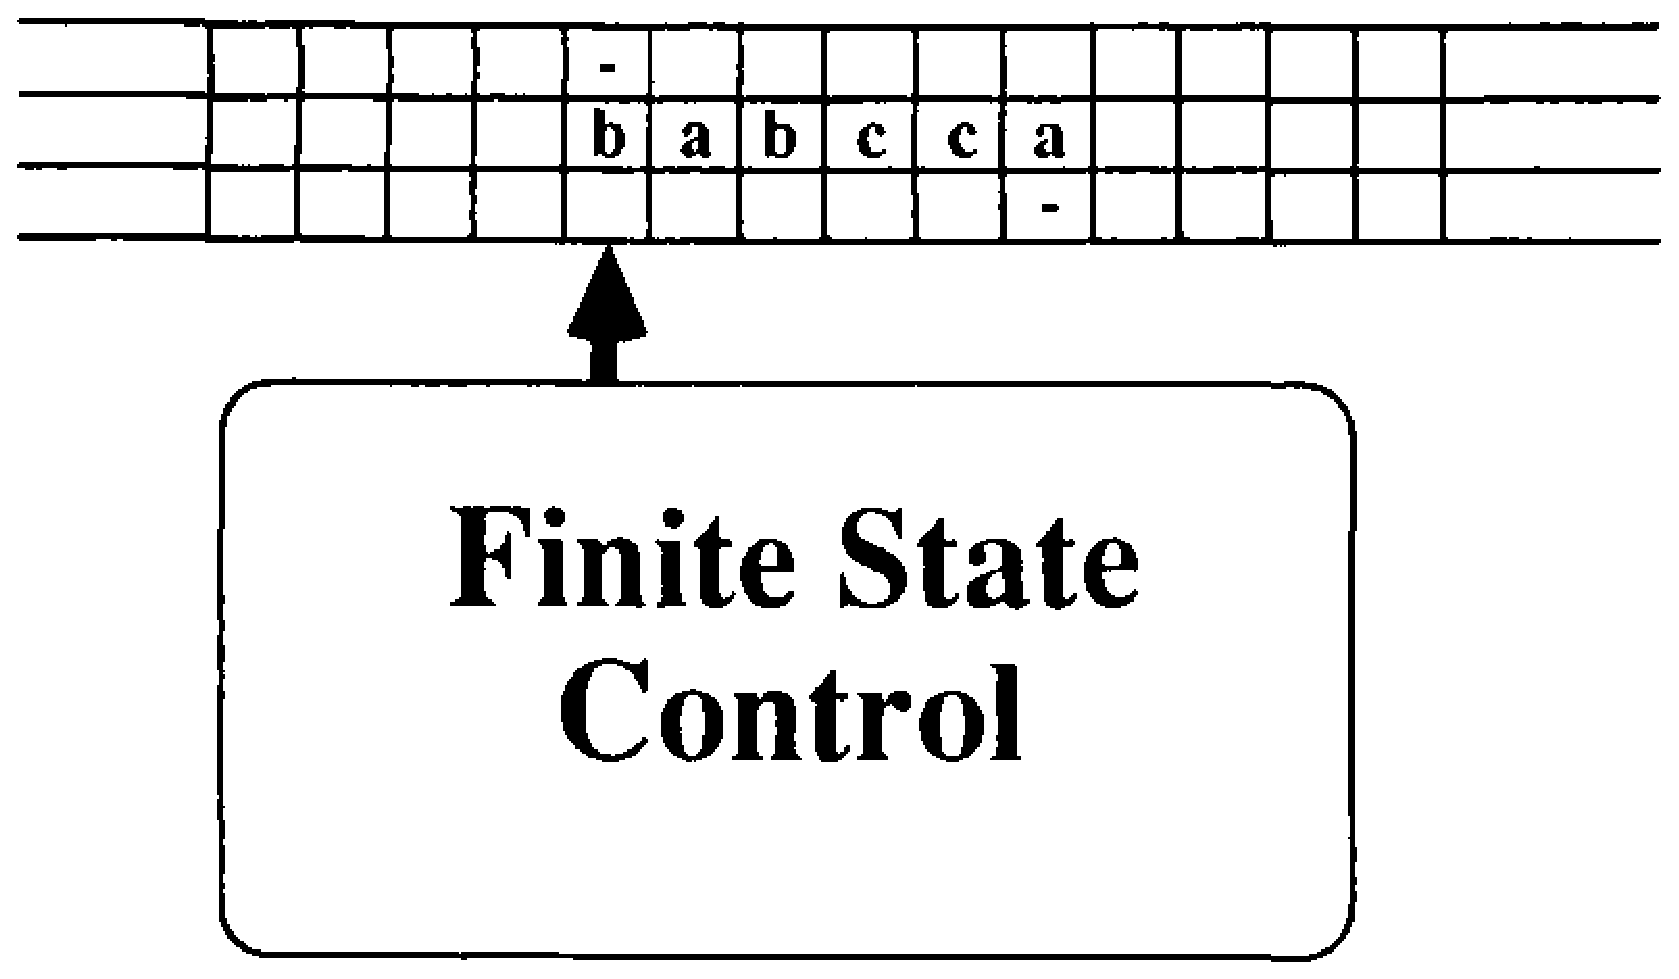
\epsfig{figure=ToFAfigures/fig11-14a.eps,width=3.4in}}
\caption{A three-track Turing machine employing delimiters}\label{fig-11.14a}
\end{figure}

% Figure 11.14b
\begin{figure}
\centerline{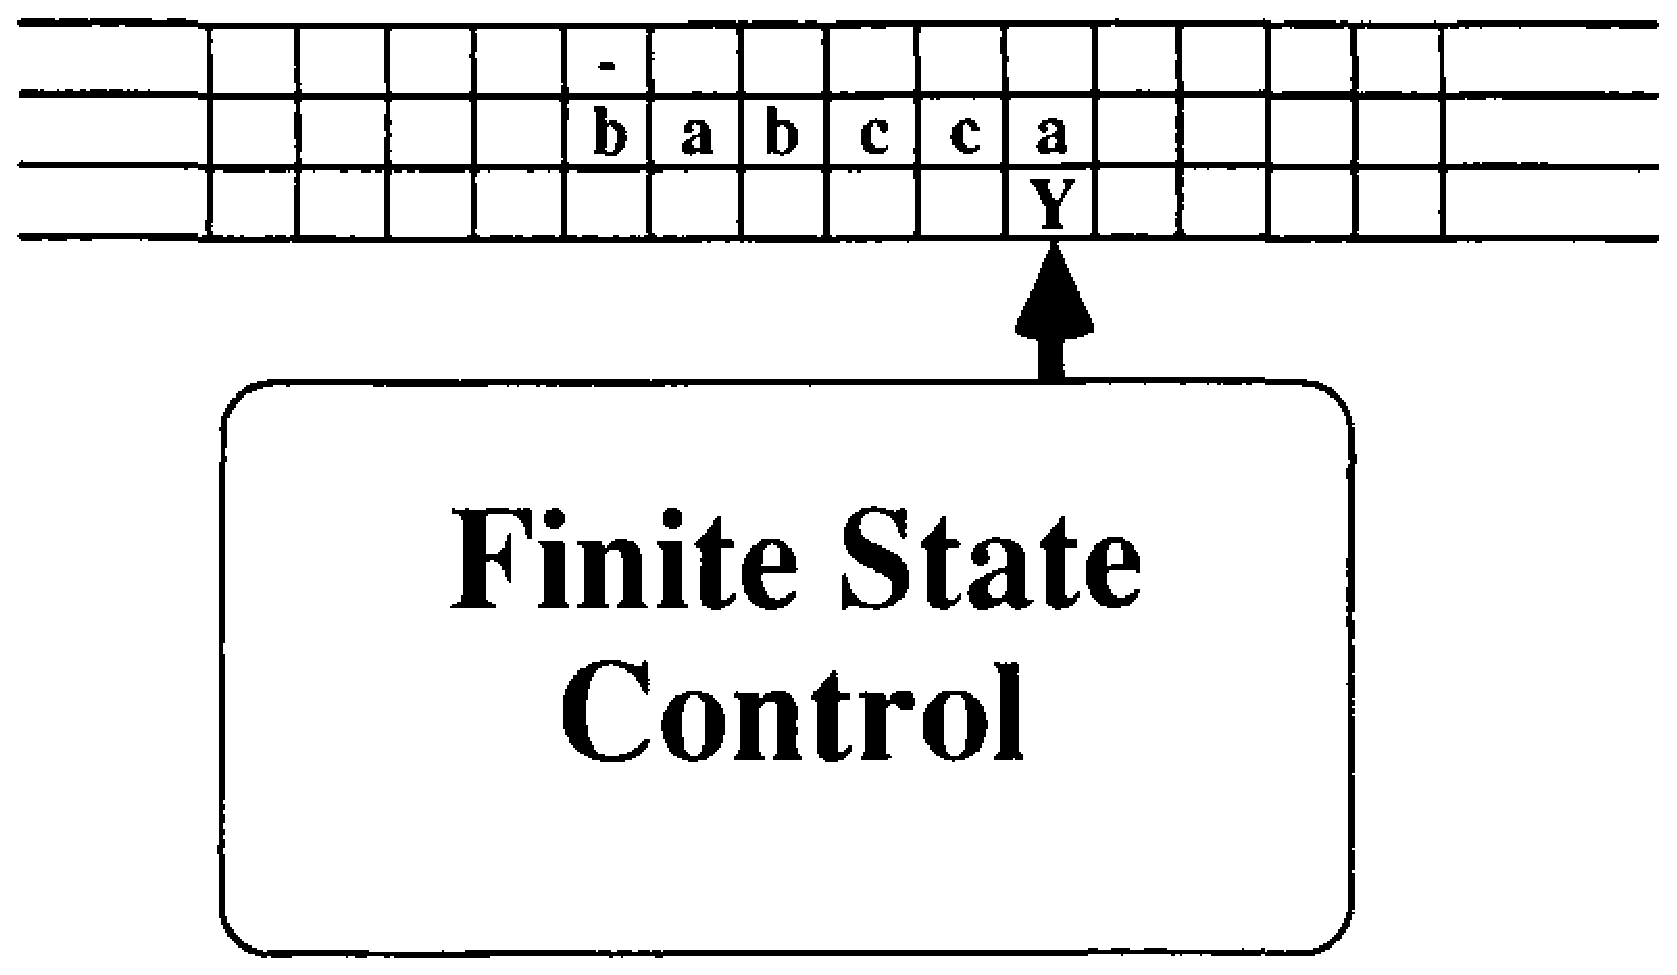
\epsfig{figure=ToFAfigures/fig11-14b.eps,width=3.4in}}
\caption{An accepting configuration}\label{fig-11.14b}
\end{figure}
\setcounter{figure}{14}                       %nasty kluge
\renewcommand{\thefigure}{\arabic{chapter}.\arabic{figure}}

\subsection*{Example 11.13}

Consider the linear-bounded automaton discussed in Example 11.10, which
accepted $\{x\in\{\pmb{a},\pmb{b},\pmb{c}\}^*|\ \ |x|_{\pmb{a}}=|x|_{\pmb{b}} =
|x|_{\pmb{c}}\}$. As suggested by the exercises, this can be modified to form
the three-track strict linear bounded automaton shown in Figure \ref{fig-11.15}, which
accepts $\{x\in\{\pmb{a},\pmb{b},\pmb{c}\}^*|\ \ |x|\geq 2\wedge |x|_{\pmb{a}} =
|x|_{\pmb{b}} = |x|_{\pmb{c}}\}$. To avoid explicitly mentioning the three
tracks, a cell containing $\pmb{b}$ on the middle track and $-$ on the upper
track is denoted by the single symbol \pmb{$\overline{b}$}, a cell containing $\pmb{A}$ on
the middle track and $-$ on the lower track is shown as \pmb{$\underline{A}$}, and so on.
Thus, the six original symbols in $\{\pmb{a},\pmb{b},\pmb{c},\pmb{A},\pmb{B},
\pmb{C}\}$ give rise to six other symbols employing the overbar $^-$, six
more using the underscore $\underline{\ \ }$, and some symbols indicating
acceptance (or possibly rejection), such as $\pmb{a}_{\pmb{Y}}$ (or $\pmb{C}_{
\pmb{N}}$). For clarity, only those combinations that can actually occur in a
transition sequence are shown in Figure \ref{fig-11.15}. The sequence of moves that would
transform the tape from the configuration shown in Figure \ref{fig-11.14a} to that of
Figure \ref{fig-11.14b} is shown below.

\begin{center}\begin{tabular}{r@{ }l@{ }l@{ }l@{ }l}
$s_0\overline{\pmb{b}}\pmb{abcc}\underline{\pmb{a}}$ & $\vdash\overline{\pmb{b}}s_1\pmb{abcc}
	\underline{\pmb{a}}$ & $\vdash\overline{\pmb{b}}s_2\pmb{Abcc}\underline{
	\pmb{a}}$ & $\vdash s_2\overline{\pmb{b}}\pmb{Abcc}\underline{\pmb{a}}$ & $\vdash$ \\
& $\ \ \ s_3\overline{\pmb{b}}\pmb{Abcc}\underline{\pmb{a}}$ & $\vdash s_4\overline{\pmb{B}}\pmb{Abcc}\underline{\pmb{a}}$ &
	$\vdash$ \\
$s_5\overline{\pmb{B}}\pmb{Abcc}\underline{\pmb{a}}$ & $\vdash\overline{\pmb{B}}s_5\pmb{Abcc}
	\underline{\pmb{a}}$ & $\vdash\overline{\pmb{B}}\pmb{A}s_5\pmb{bcc}\underline{\pmb{a}}$ &
	$\vdash\overline{\pmb{B}}\pmb{Ab}s_5\pmb{cc}\underline{\pmb{a}}$ & $\vdash$ \\
$\overline{\pmb{B}}\pmb{Ab}s_6\pmb{Cc}\underline{\pmb{a}}$ & $\vdash\overline{\pmb{B}}\pmb{A}s_6\pmb{bCc}
	\underline{\pmb{a}}$ & $\vdash\overline{\pmb{B}}s_6\pmb{AbCc}\underline{\pmb{a}}$ &
	$\vdash s_6\overline{\pmb{B}}\pmb{AbCc}\underline{\pmb{a}}$ & $\vdash$ \\
& $\ \ \ s_0\overline{\pmb{B}}\pmb{AbCc}\underline{\pmb{a}}$ & $\vdash\overline{\pmb{B}}s_0\pmb{Ab
	Cc}\underline{\pmb{a}}$ & $\vdash\overline{\pmb{B}}\pmb{A}s_0\pmb{bCc}\underline{\pmb{a}}$
	& $\vdash$ \\
$\overline{\pmb{B}}\pmb{Ab}s_1\pmb{Cc}\underline{\pmb{a}}$ && $\Dvdash s_2\overline{\pmb{B}}
	\pmb{AbCc}\underline{\pmb{A}}$ && $\Dvdash$ \\
$\overline{\pmb{B}}\pmb{A}s_3\pmb{bCc}\underline{\pmb{A}}$ && $\Dvdash s_4\overline{\pmb{B}}
	\pmb{ABCc}\underline{\pmb{A}}$ && $\Dvdash$ \\
$\overline{\pmb{B}}\pmb{ABC}s_5\pmb{c}\underline{\pmb{A}}$ && $\Dvdash s_6\overline{\pmb{B}}
	\pmb{ABCC}\underline{\pmb{A}}$ && $\Dvdash$ \\
& $\ \ \ \overline{\pmb{B}}\pmb{ABCC}s_0\underline{\pmb{A}}$ & $\vdash\overline{\pmb{B}}\pmb{ABCC}
	s_7\underline{\pmb{a}}$ & $\vdash\overline{\pmb{B}}\pmb{ABC}s_7\pmb{C}
	\underline{\pmb{a}}$ & $\vdash$ \\
$\overline{\pmb{B}}\pmb{ABC}s_7\pmb{c}\underline{\pmb{a}}$ && $\Dvdash s_7\overline{\pmb{B}}
	\pmb{abcc}\underline{\pmb{a}}$ && $\vdash$ \\
$s_8\overline{\pmb{b}}\pmb{abcc}\underline{\pmb{a}}$ & $\vdash\overline{\pmb{b}}s_8\pmb{abcc}
	\underline{\pmb{a}}$ & $\Dvdash\overline{\pmb{b}}\pmb{abcc}s_8\underline{\pmb{a}}$
	&& $\vdash$ \\
$\overline{\pmb{b}}\pmb{abcc}h\pmb{a_{Y}}$
\end{tabular}\end{center}

Consider implementing a grammar similar to that given in Definition \ref{dfn-11.8}, but
applied to a strict linear bounded automaton incorporating the two delimiting
markers on separate tracks. The new symbols will eliminate the need for $[$ and
$]$ and avoid the contracting productions that were required to delete $[$ and
$]$ from the sentential form. The class 3 productions would simply replace a
symbol such as $\pmb{a}_{\pmb{Y}}$ with $\pmb{a}$ and $\overline{\pmb{b}}$ with
$\pmb{b}$.

Unfortunately, it will not be possible to explicitly use distinct symbols to
keep track of the state and the placement of the state head, as was done with
$s_0,s_1,\ldots,s_n$, and $h$ in the previous production sets. This extraneous
symbol will also have to disappear to form a terminal string, and this must be
done in a way that does not use contracting productions. As with the underscore
and overbar, the state name will be encoded as a subscript attached to one
symbol in the sentential form. Thus, each original symbol $\pmb{d}$, which has
already given rise to additional nonterminals $\overline{\pmb{d}}$ and
$\underline{\pmb{d}}$, will also require nonterminals such as $\pmb{d}_0,\pmb{d}_1,
\ldots,\pmb{d}_n$ to be added to $\Gamma$. The inclusion of $\pmb{d}_i$ within a
sentential form will reflect that the tape head is currently scanning this
$\pmb{d}$ while the finite-state control is in state $s_i$. Further symbols will
also be needed; $\overline{\pmb{d}}_i$ indicates that the tape head is scanning
the leftmost symbol, which happens to be $\pmb{d}$, while the finite-state
control is in state $s_i$, and $\pmb{\underline{d}}_i$ indicates a similar
situation involving the rightmost symbol.

This plethora of nonterminals can be used to define a context-sensitive grammar
that generates the language recognized by a strict linear bounded automaton.
For the automaton given in Example 11.13, generating the terminal string
${\pmb{b}}\pmb{abcca}$ will begin with the random generations of the
six-symbol sentential form $\overline{\pmb{b}}_0\pmb{abcc}\underline{\pmb{a}}$ with the class 1
productions, which will be transformed into $\overline{\pmb{b}}\pmb{abcca_{Y}}$
by the class 2 productions, and finally into $\pmb{babcca}$ via the class 3
productions. In the following definition, note that by the conditions placed on
a strict linear bounded automaton $\Gamma$ already contains symbols of the form
$\overline{\pmb{A}}$ and $\underline{\pmb{A}}$, and hence so will $\Gamma_{\!\!B}$.
For simplicity, the state set is required to be of the form $\{s_0,s_1,\ldots,
s_n\}$, but clearly the state names of any automaton could be renumbered
sequentially to fit the given definition.

% Figure 11.15
\begin{figure}
\centerline{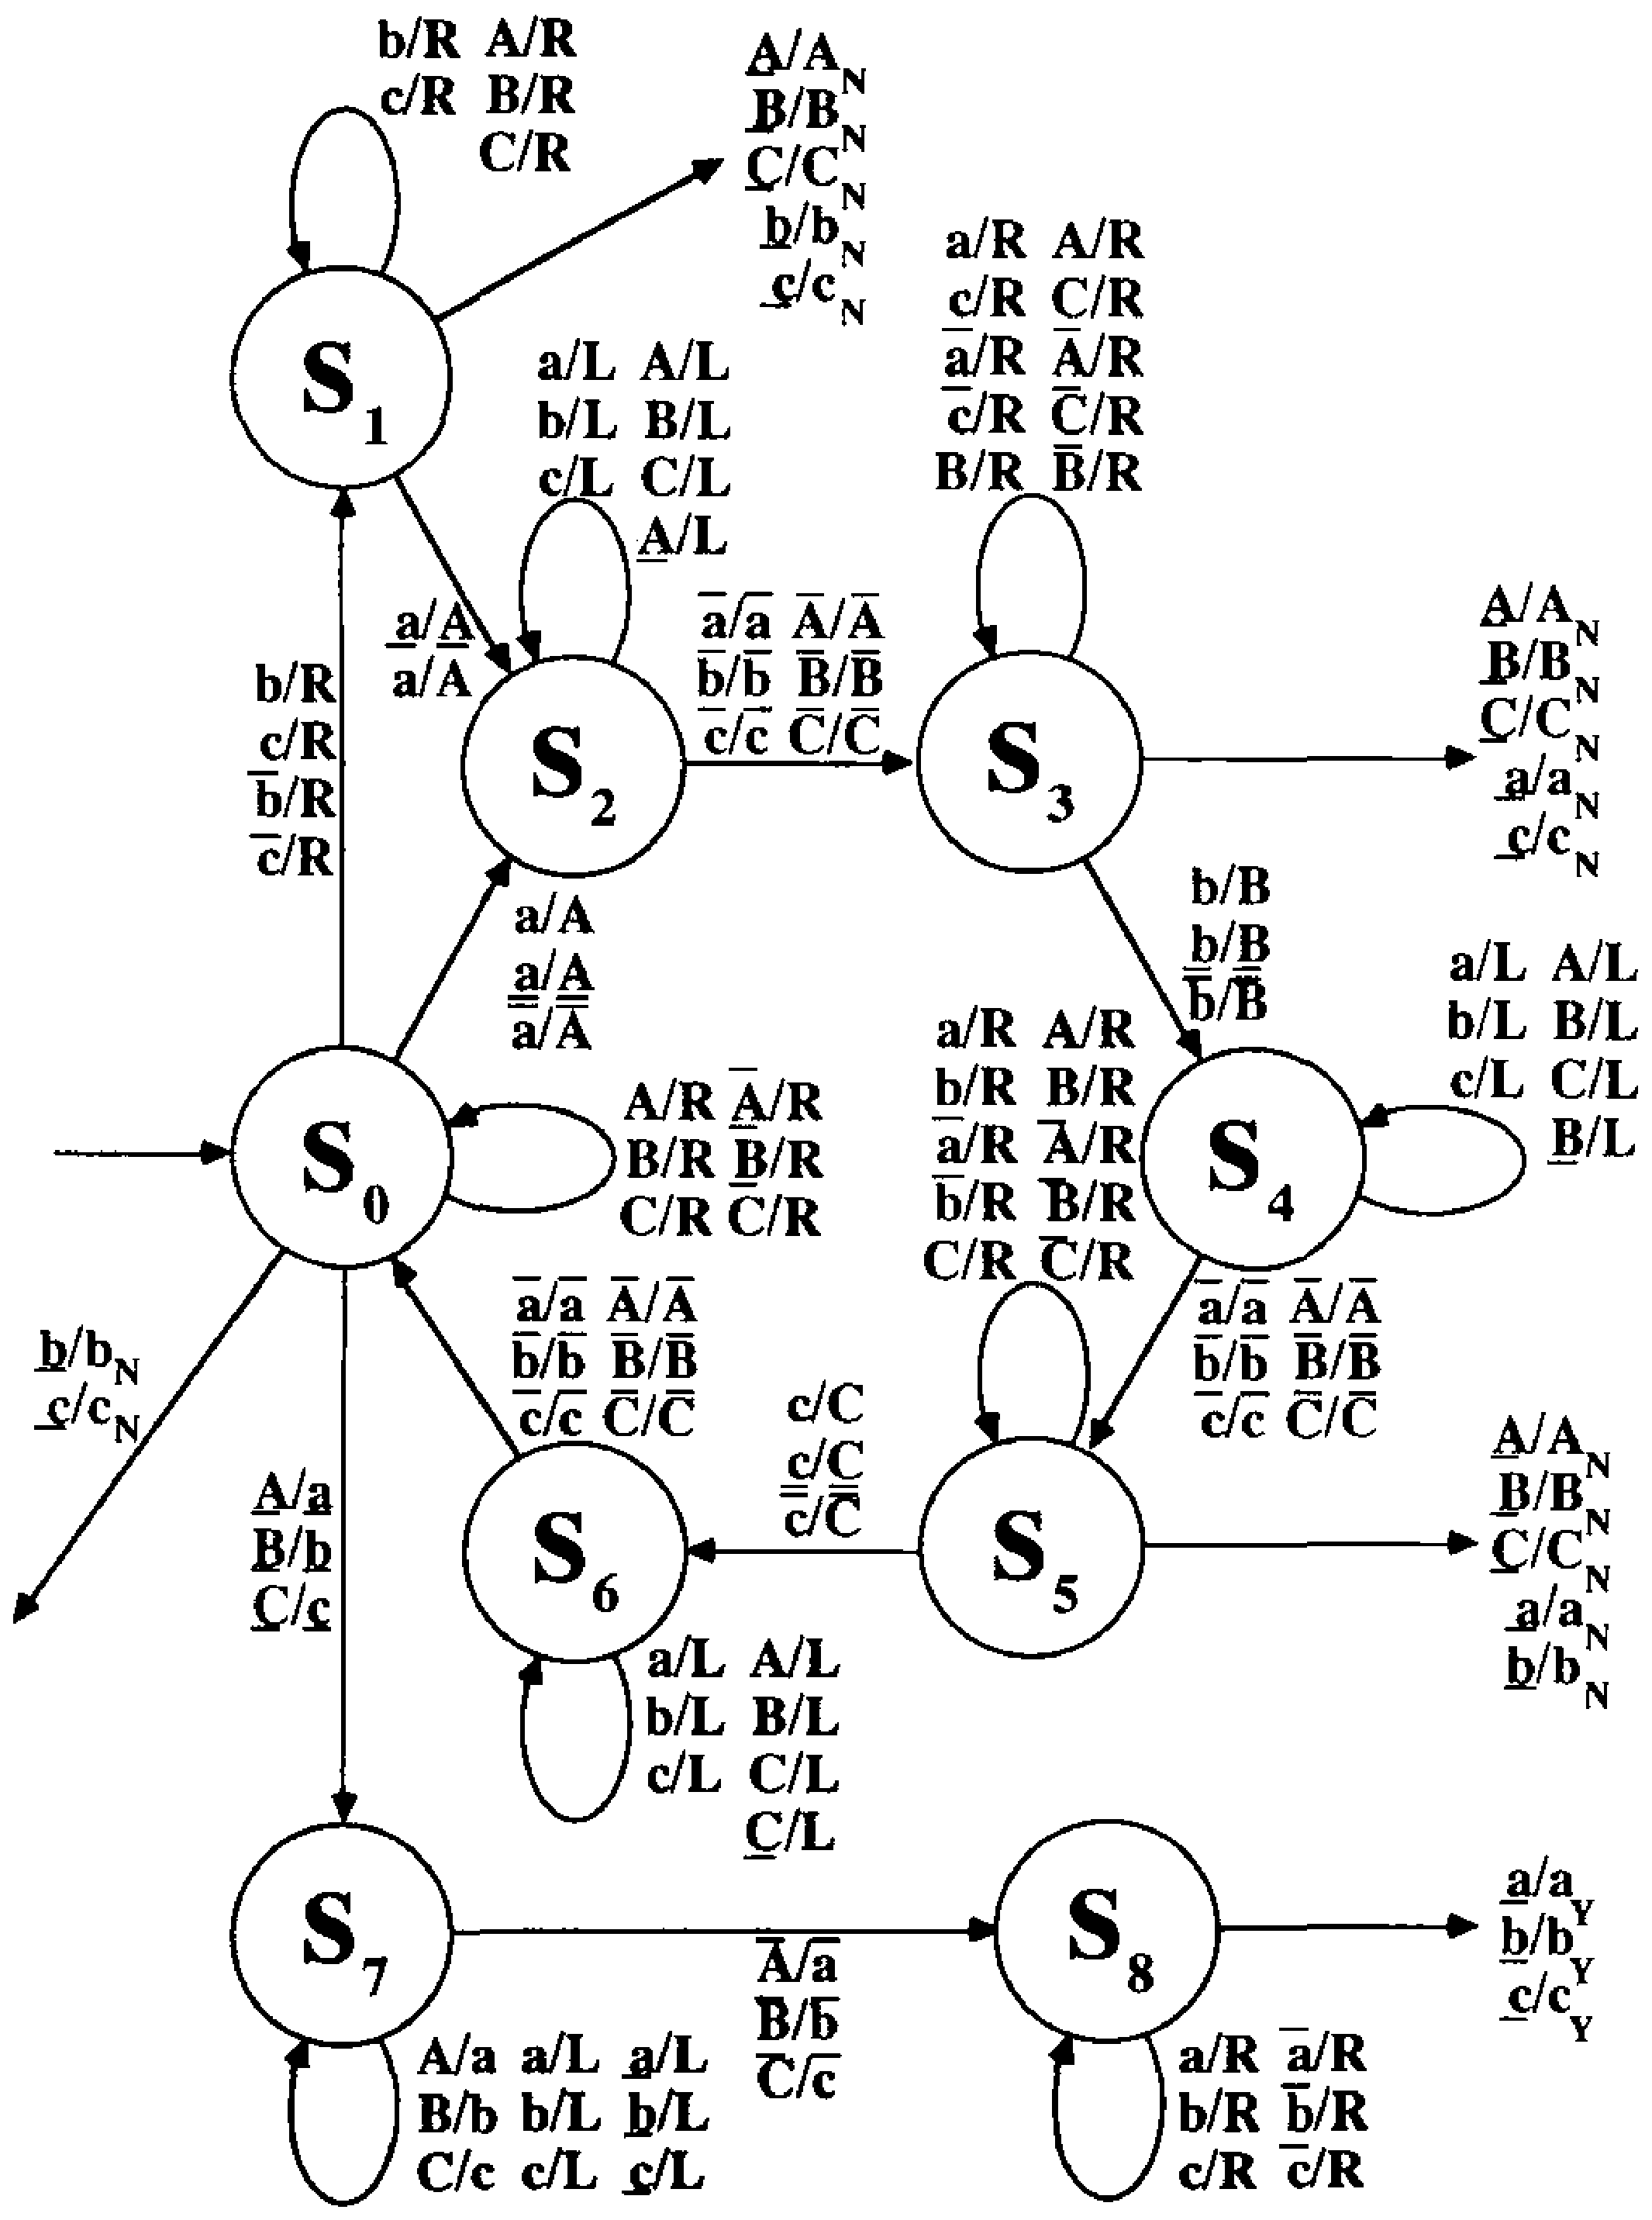
\epsfig{figure=ToFAfigures/fig11-15.eps,height=3.8in}}
\caption{The Turing machine discussed in Example 11.13}\label{fig-11.15}
\end{figure}

% Definition 11.9
\begin{dfn}\label{dfn-11.9}
Given a strict linear bounded automaton
\[ B=\langle\Sigma,\Gamma,\{s_0,s_1,\ldots,s_n\},s_0,\delta\rangle, \]
the context-sensitive grammar corresponding to $B$, $G_B$, is given by
\[ G_B=\langle\Sigma,\Gamma_{\!\!B},Z,P_B\rangle, \]
where $\Gamma_{\!\!B}$ is given by
\[ \Gamma_{\!\!B}=\Gamma\cup\{\pmb{d}_i|\ \pmb{d}\in\Sigma\cup\Gamma,i=1,2,\ldots,n,
	\text{ or }i=\pmb{Y}\}\cup\{Z,S,W\} \]

$P_B$ contains the following classes of productions:
\begin{enumerate}
\item If $\lambda\in L(B)$, then $Z\rightarrow\lambda\in P_B$ \\
$Z\rightarrow S\in P_B$ \\
$(\forall\pmb{d}\in\Sigma)($if $\pmb{d}\in L(B)$, then $S\rightarrow\pmb{d}\in
P_B)$ \\
$(\forall\pmb{d}\in\Sigma)(S\rightarrow W\underline{\pmb{d}}\in P_B)$ \\
$(\forall\pmb{d}\in\Sigma)(W\rightarrow W\pmb{d}\in P_B)$ \\
$(\forall\pmb{d}\in\Sigma)(W\rightarrow\overline{\pmb{d}}_0\in P_B)$
\item Each printing transition gives rise to a production rule as follows:
\[ (\forall s_i,s_j\in S)(\forall\pmb{a},\pmb{b}\in\Sigma\cup\Gamma)(\text{ if }
	\delta(s_i,\pmb{a})=\langle s_j,\pmb{b}\rangle,\text{ then }\pmb{a}_i
	\rightarrow\pmb{b}_j\in P_B) \]
Each move right gives rise to a production rule as follows:
\[ (\forall s_i,s_j\in S)(\forall\pmb{a}\in\Sigma\cup\Gamma)(\text{if }\delta(
	s_i,\pmb{a}) = \langle s_j,\pmb{R}\rangle,\text{ then }(\forall\pmb{d}
	\in\Sigma\cup\Gamma)(\pmb{a}_i\pmb{d}\rightarrow\pmb{ad}_j\in P_B)) \]
Each move left gives rise to a production rule as follows:
\[ (\forall s_i,s_j\in S)(\forall\pmb{a}\in\Sigma\cup\Gamma)(\text{if }\delta(
	s_i,\pmb{a})=\langle s_j,\pmb{L}\rangle,\text{ then }(\forall\pmb{d}\in
	\Sigma\cup\Gamma)(\pmb{da}_i\rightarrow\pmb{d}_j\pmb{a}\in P_B)) \]
Each halt with acceptance gives rise to a production rule as follows:
\[ (\forall s_i\in S)(\forall\pmb{b}\in\Sigma\cup\Gamma)(\forall\pmb{a}\in\Sigma)
	(\text{if }\delta(s_i,\pmb{b})=\langle h,\pmb{a}_{\pmb{Y}}\rangle,
	\text{ then }\pmb{b}_i\rightarrow\pmb{a}_{\pmb{Y}}\in P_B) \]
\item $(\forall\pmb{a},\pmb{b}\in\Sigma)(\pmb{ba}_{\pmb{Y}}\rightarrow\pmb{b}_{
	\pmb{Y}}\pmb{a}\in P_B)$ \\
$(\forall\pmb{a},\pmb{b}\in\Sigma)(\overline{\pmb{b}}\pmb{a}_{\pmb{Y}}\rightarrow
	\pmb{ba}\in P_B)$
\end{enumerate}
\end{dfn}

\subsection*{Example 11.14}

Consider again the strict linear bounded automaton $B$ given in Figure \ref{fig-11.15} and
the corresponding context-sensitive grammar $G_B$. The following derivation
sequences show that $\pmb{babcca}\in L(G_B)$:
\[ Z\Rightarrow S\Rightarrow W\underline{\pmb{a}}\Rightarrow W\pmb{c}\underline{\pmb{a}}
	\Rightarrow W\pmb{cc}\underline{\pmb{a}}\Rightarrow W\pmb{bcc}\underline{\pmb{a}}
	\Rightarrow W\pmb{abcc}\underline{\pmb{a}}\Rightarrow\overline{\pmb{b}}_0
	\pmb{abcc}\underline{\pmb{a}} \]
At this point, only the class 2 productions can be employed, yielding:
\begin{center}\begin{tabular}{r@{ }l@{ }l@{ }l@{ }l}
$\overline{\pmb{b}}_0\pmb{abcc}\underline{\pmb{a}}$ & $\Rightarrow\overline{\pmb{b}}\pmb{a}
	_1\pmb{bcc}\underline{\pmb{a}}$ & $\Rightarrow\overline{\pmb{b}}\pmb{A}_2\pmb{bcc}
	\underline{\pmb{a}}$ & $\Rightarrow\overline{\pmb{b}}_2\pmb{Abcc}\underline{\pmb{a}}$ &
	$\Rightarrow$ \\
& $\ \ \ \ \ \overline{\pmb{b}}_3\pmb{Abcc}\underline{\pmb{a}}$ & $\Rightarrow
	\overline{\pmb{B}}_4\pmb{Abcc}\underline{\pmb{a}}$ && $\Rightarrow$ \\
$\overline{\pmb{B}}_5\pmb{Abcc}\underline{\pmb{a}}$ & $\Rightarrow\overline{\pmb{B}}
	\pmb{A}_5\pmb{bcc}\underline{\pmb{a}}$ & $\Rightarrow\overline{\pmb{B}}\pmb{Ab}_5\pmb{cc}
	\underline{\pmb{a}}$ & $\Rightarrow\overline{\pmb{B}}\pmb{Abc}_5\pmb{c}\underline{\pmb{a}}$
	& $\Rightarrow$ \\
$\overline{\pmb{B}}\pmb{AbC}_6\pmb{c}\underline{\pmb{a}}$ & $\Rightarrow\overline{\pmb{B}}\pmb{Ab}
	_6\pmb{Cc}\underline{\pmb{a}}$ & $\Rightarrow\overline{\pmb{B}}\pmb{A}_6\pmb{bCc}
	\underline{\pmb{a}}$ & $\Rightarrow\overline{\pmb{B}}_6\pmb{AbCc}\underline{\pmb{a}}$
	& $\Rightarrow$ \\
& $\ \ \ \ \ \overline{\pmb{B}}_0\pmb{AbCc}\underline{\pmb{a}}$ & $\Rightarrow
	\overline{\pmb{B}}\pmb{A}_0\pmb{bCc}\underline{\pmb{a}}$ & $\Rightarrow\overline{\pmb{B}}
	\pmb{Ab}_0\pmb{Cc}\underline{\pmb{a}}$ & $\Rightarrow$ \\
$\overline{\pmb{B}}\pmb{AbC}_1\pmb{c}\underline{\pmb{a}}$ && $\DRightarrow\overline{\pmb{B}}
	_2\pmb{AbCc}\underline{\pmb{A}}$ && $\DRightarrow$ \\
$\overline{\pmb{B}}\pmb{Ab}_3\pmb{Cc}\underline{\pmb{A}}$ && $\DRightarrow\overline{\pmb{B}}
	_4\pmb{ABCc}\underline{\pmb{A}}$ && $\DRightarrow$ \\
$\overline{\pmb{B}}\pmb{ABCc}_5\underline{\pmb{A}}$ && $\DRightarrow\overline{\pmb{B}}
	_6\pmb{ABCC}\underline{\pmb{A}}$ && $\DRightarrow$ \\
& $\ \ \ \ \ \overline{\pmb{B}}\pmb{ABCC}\underline{\pmb{A}}_0$ & $\Rightarrow
	\overline{\pmb{B}}\pmb{ABCC}\underline{\pmb{a}}_7$ & $\Rightarrow\overline{\pmb{B}}\pmb{ABCC}_7
	\underline{\pmb{a}}$ & $\Rightarrow$ \\
$\overline{\pmb{B}}\pmb{ABCc}_7\underline{\pmb{a}}$ && $\DRightarrow\overline{\pmb{B}}
	_7\pmb{abcc}\underline{\pmb{a}}$ && $\Rightarrow$ \\
$\overline{\pmb{b}}_8\pmb{abcc}\underline{\pmb{a}}$ & $\Rightarrow\overline{\pmb{b}}\pmb{a}
	_8\pmb{bcc}\underline{\pmb{a}}$ & $\DRightarrow\overline{\pmb{b}}\pmb{abcc}
	\underline{\pmb{a}}_8$
\end{tabular}\end{center}
Finally, since $\delta(s_8,\underline{\pmb{a}})=\langle h,\pmb{a_Y}\rangle$,
the class 3 productions can then be applied:
\[ \overline{\pmb{b}}\pmb{abcc}\underline{\pmb{a}}_8\Rightarrow\overline{\pmb{b}}\pmb{abcca_Y}
	\Rightarrow\overline{\pmb{b}}\pmb{abcc_Ya}\Rightarrow\overline{\pmb{b}}\pmb{abc_Yca}
	\Rightarrow\overline{\pmb{b}}\pmb{ab_Ycca}\Rightarrow\overline{\pmb{b}}\pmb{a_Ybcca}
	\Rightarrow\pmb{babcca} \]

Once again, the grammars springing from Definition \ref{dfn-11.9} can generate sentential
forms corresponding to any string in $\Sigma^*$, as long as the length of the
string is at least two. As with the grammars arising from Definition \ref{dfn-11.8}, only
strings that would have been accepted by the original machine will lead to a
terminal string. If the productions of this example were applied to the
sentential form $\overline{\pmb{b}}_0\pmb{a}\underline{\pmb{a}}$, at each step there
will be exactly one choice of applicable production, until eventually the form
$\overline{\pmb{B}}\pmb{A}\underline{\pmb{a}}_5$ is obtained. At this step, no production will
apply, and therefore a terminal string cannot be generated from $\overline{\pmb{
b}}_0\pmb{a}\underline{\pmb{a}}$. This correspondence between words accepted by the
machine $B$ and words generated by the context-sensitive grammar $G_B$
given in Definition \ref{dfn-11.9} is the foundation of the following theorem.

% Theorem 11.5
\begin{thm}\label{thm-11.5}
Let $\Sigma$ be an alphabet. Then $\LSIG\subseteq\OSIG$. That is, every linear
bounded language can be generated by a type 1 grammar.

\emph{Proof.} Any linear bounded language can be recognized by a strict linear
bounded automaton (see the exercises). Hence, if $L$ is a linear bounded
language, there exists a strict linear bounded automaton $B=\langle\Sigma,
\Gamma,\{s_0,s_1,\ldots,s_n\},s_0,\delta\rangle$ which accepts exactly the words
in $L$ by printing $\pmb{Y}$ on the lowest of the three tracks after restoring
the original word to the middle track. We will employ the grammar $G_B$
corresponding to $B$, as given in Definition \ref{dfn-11.9}. Example 11.14 illustrated
that these productions can be used in a manner similar to those of Definition
\ref{dfn-11.8}, and it is easy to justify that they cannot be combined in unexpected ways.
Induction on the length of $x$ will show that by using just the productions in
class 1,
\[ (\forall x\in\Sigma^*)(\forall\pmb{a},\pmb{b}\in\Sigma)(Z\ \DRightarrow
	\overline{\pmb{a}}_0x\underline{\pmb{b}}) \]

The correspondence between sequences of applications of the class 2 productions
and sequences of moves in $B$ follows as in Theorem \ref{thm-11.4}. Due to the myriad
positions that the integer subscript can occupy, and the special cases caused
by the presence of the overbars and underscores, the general induction statement
is quite tedious to state and is left as an exercise. The statement will again
be applied to the special case in which we are interested, as stated below.
\[ (\forall x\in\Sigma^*)(\forall\pmb{a},\pmb{b}\in\Sigma)(s_0\pmb{a}x\pmb{b}
	\Dvdash\pmb{a}xh\pmb{b_Y}\text{\ \ iff\ \ \ \ }\overline{\pmb{a}}_0x
	\underline{\pmb{b}}\ \ \DRightarrow\ \overline{\pmb{a}}x\pmb{b_Y}) \]
A final induction argument will show that $\overline{\pmb{a}}x\pmb{b_Y}
\DRightarrow\pmb{a}x\pmb{b}$. Thus,
\[ (\forall x\in\Sigma^*)(\forall\pmb{a},\pmb{b}\in\Sigma)(s_0\pmb{a}x\pmb{b}
	\Dvdash\pmb{a}xh\pmb{b_Y}\text{\ \ iff\ \ } Z\ \DRightarrow
	\overline{\pmb{a}}_0x\underline{\pmb{b}}\ \ \DRightarrow\overline{\pmb{a}}x
	\pmb{b_Y}\ \DRightarrow\ \pmb{a}x\pmb{b}) \]
This establishes the correspondence between words \emph{of length at least two}
accepted by $B$ and those generated by $G_B$. Definition \ref{dfn-11.9} included specific
productions of the form $Z\rightarrow\lambda$ and $S\rightarrow\pmb{d}$ to
ensure that words of length 0 and 1 also corresponded. This implies that $L(B)=
L(G_B)$, as was to be shown.
\end{thm}

The proof of Theorem \ref{thm-11.5} argues that there exists a context-sensitive grammar
$G_B$ for each strict linear bounded automaton $B$, and it certainly appears
that given an automaton $B$ we can immediately write down all the productions in
$P_B$, as specified by Definition \ref{dfn-11.9}. However, some of the class 1 productions
may cause some trouble. For example, determining whether the production $Z
\rightarrow\lambda$ is included in $P_B$ depends on whether the automaton halts
with $\pmb{Y}$ when presented with a blank tape. In the next chapter, we will
see that even this simple question cannot be effectively answered for arbitrary
Turing machines! That is, it is impossible to find an algorithm that, when
presented with the state diagram of a Turing machine, can reliably determine
whether or not the machine accepts the empty string. It will be shown that any
such proposed algorithm is guaranteed to give the wrong answer for some Turing
machines. Similarly, it now seems that there might be some uncertainty about
which members of $\Sigma$ give rise to productions of the form $S\rightarrow
\pmb{d}$.

The productions specified by Definition \ref{dfn-11.9} were otherwise quite explicit; only
the productions relating to the immediate generation of a single character or
the empty string were in any way questionable. There are only $|\Sigma|+1$ such
productions, and some combination of them has to be the correct set of
productions to include in $P_B$. Thus, as stated in the theorem, we \emph{are}
assured that a context-sensitive grammar does exist, even if we are unclear as
to exactly which of these special productions it should contain.

As will be seen in Chapter \ref{ch-12}, it \emph{is} possible to determine which words
are accepted (and which are rejected) by linear bounded automata. Unlike
unrestricted Turing machines, there is only a finite span of tape upon which
symbols can be placed. Furthermore, there are only a finite number of characters
that can appear in those cells, a finite number of positions the tape head can
be in, and a finite number of states to consider. The limited number of
configurations makes it possible to determine exactly which words of a given
size are recognized by the LBA.

We have seen that every linear bounded automaton is equivalent to a strict
linear bounded automaton, and these have equivalent type 1 grammars. Conversely,
every type 1 grammar generates a linear bounded language, which implies there is
another correspondence between a generative construct and a cognitive construct.

% Corollary 11.2
\begin{cor}\label{cor-11.2}
The class of languages generated by context-sensitive grammars is exactly the
linear bounded languages. That is, $\LSIG=\OSIG$.

\emph{Proof.} The proof follows immediately from Theorems \ref{thm-11.3} and \ref{thm-11.5}.
\end{cor}

\section{Closure Properties and The Hierarchy Theorem}\label{sec-11.4}

Finally, we consider some of the closure properties of the classes of languages
explored in this chapter. Since $\TSIG=\ZSIG$ we may use either cognitive or
generative constructs for this class, whichever is most convenient. The fact
that $\LSIG=\OSIG$, will allow similar freedom for the type 1 languages. The
next theorem illustrates a case in which the grammatical construct is the
easier to use.

% Theorem 11.6
\begin{thm}\label{thm-11.6}
Let $\Sigma$ be an alphabet. Then $\TSIG$, is closed under union.

\emph{Proof.} If $L_1$ and $L_2$ are two Turing-acceptable languages, then by
Theorem \ref{thm-11.4} there are type 0 grammars $G_1=\langle\Omega_1,\Sigma,S_1,P_1
\rangle$ and $G_2=\langle\Omega_2,\Sigma,S_2,P_2\rangle$ that recognize $L_1$
and $L_2$. Without loss of generality, assume that $\Omega_1\cap\Omega_2=
\emptyset$. Choose a new nonterminal $Z$ such that $Z\notin\Omega_1\cup\Omega_2$,
and consider the new type 0 grammar $G^{\cup}$ defined by $G^{\cup}=\langle
\Omega_1\cup\Omega_2\cup\{Z\},\Sigma,Z,P_1\cup P_2\cup\{Z\rightarrow S_1,Z
\rightarrow S_2\}\rangle$. Clearly, $L(G^{\cup})=L(G_1)\cup L(G_2)$. By Theorem
\ref{thm-11.2}, there is a Turing machine equivalent to $G^{\cup}$, and hence $L_1\cup
L_2$ is Turing acceptable.
\end{thm}

Theorem \ref{thm-11.6} could be proved directly by constructing a new Turing machine
from Turing machines $T_1$ and $T_2$ accepting $L_1$ and $L_2$. It is a bit
harder to give a concrete proof and care must be taken to avoid inappropriate
constructions. For example, it would be incorrect to build the new machine in
such a way that it first simulates $T_1$ halting with $\pmb{Y}$ if $T_1$ does,
and then simulating $T_2$ if $T_1$ would have halted with $\pmb{N}$. It must be
remembered that there is no guarantee that a Turing machine will \emph{ever}
halt for a given word. The above construction will incorrectly reject words that
could be recognized by $T_2$ but which were rejected by $T_1$ because $T_1$
never halted; the new machine would never get a chance to simulate $T_2$. One
valid construction involves a two-tape Turing machine, which immediately copies
the input word onto the second tape. By using a \Index{cross product} of the states of
$T_1$ and $T_2$ and appropriate transitions, the action of both machines
could be simultaneously simulated, and the new machine would accept as soon as
either simulation indicated that the word should be accepted. A slight
modification of this construct would show that \TSIG\ is also closed under
intersection, but the next theorem outlines a superior method.

% Theorem 11.7
\begin{thm}\label{thm-11.7}
Let $\Sigma$ be an alphabet. Then \TSIG\ is closed under intersection.

\emph{Proof.} $L_1$ and $L_2$ are two Turing-acceptable languages recognized by
the Turing machines $T_1$ and $T_2$, respectively. We build a new Turing machine
$T^{\cap}$ with $T_1$ and $T_2$ as submachines. $T^{\cap}$ transfers control to
the submachine $T_1$. If $T_1$ never halts, the input will be rejected, which is
the desired result. If $T_1$ halts, $T^{\cap}$ erases the $\pmb{Y}$ and moves
the tape head back to the leftmost character and transfers control to the
submachine $T_2$. $T^{\cap}$ will halt if $T_2$ does, and if $T_2$ also accepts,
$\pmb{Y}$ will be left in the proper place on the tape. $T^{\cap}$ therefore
accepts if and only if both $T_1$ and $T_2$ accept, and hence $L_1\cap L_2$ is
Turing acceptable.
\end{thm}

Note that it was important that, except for the presence of $\pmb{Y}$ after the
input word, $T_1$ left the tape in the same condition it found it, with the
input string intact for $T_2$. As with type 3 and type 2 grammars, there is no
pleasant way to combine type 0 grammars to produce a grammar that generates the
intersection of type 0 languages, although Theorem \ref{thm-11.7} guarantees (along with Corollary \ref{cor-11.1}) that such a
grammar must surely exist.

% Theorem 11.8
\begin{thm}\label{thm-11.8}
Let $\Sigma$ be an alphabet. Then \TSIG\ is closed under reversal, homomorphism,
inverse homomorphism, substitution, concatenation, and Kleene closure.

\emph{Proof.} The proof for reversal is almost trivial; it is almost as simple
as replacing every transition that moves the tape head to the right with a
transition to the left, and likewise making left moves into right moves. This
will yield a mirror image machine, which when started at the \emph{right}most
character will print $\pmb{Y}$ just past the \emph{left}most character. We
therefore have to modify this machine by adding preliminary states that will
move the tape head from its traditional leftmost starting position to the
opposite end of the word. Similarly, just before the $\pmb{Y}$ would be printed,
we must again move the tape head to the right.

The description of the modifications necessary to convert a type 0 grammar into
one that generates the reverse of the original is even more succinct: Each rule
in the original grammar is modified by writing the characters to the left of the
production symbol $\rightarrow$ backward, and similarly reversing the string on
the right of $\rightarrow$. That is, a production like $\pmb{Dc}\rightarrow
\pmb{ABe}$ would become $\pmb{cD}\rightarrow\pmb{eBA}$. A relatively trivial
induction on the number of steps in a derivation proves that the new grammar
accepts the reverse of the original language. The proofs of closure under the
remaining operators are left for the exercises.
\end{thm}

As shown in Chapter \ref{ch-12}, there are some operators under which \TSIG\ is not
closed. Complementation is perhaps the most glaring exception. The closure
properties of \LSIG\ are very similar to those of \TSIG. In most cases, slight
modifications of the above proofs carry over to the type 1 languages.

% Theorem 11.9
\begin{thm}\label{thm-11.9}
Let $\Sigma$ be an alphabet. Then \OSIG\ is closed under reversal, homomorphism,
inverse homomorphism, substitution, concatenation, union, and intersection.

\emph{Proof.} Both proofs given for reversal carry over without modification. In
the cognitive approach, the states added to the mirror image Turing machine keep
the tape head within the confines of the input word, and hence if the original
machine was a LBA, the new version will also be a LBA. In the generative
approach, reversing the characters in type 1 productions still results in a type
1 grammar. That is, if the original grammar had no contracting productions,
neither will the new grammar.

Proving that the union of two type 1 languages is type 1 is similar to the
proof given in Theorem \ref{thm-11.6}, although care must be taken to avoid extraneous
productions of the form $Z_1\rightarrow\lambda$. Building an intersection
machine from two linear bounded automata can be done exactly as described in
Theorem \ref{thm-11.7}. The remaining closure properties are left for the exercises.
\end{thm}

It is clear from our definitions that $\OSIG\subseteq\ZSIG$, but we have yet to
prove that $\OSIG\subset\ZSIG$. That the inclusion is proper and \ZSIG\ is truly
a larger class than \OSIG\ will be shown to be a consequence of the material
considered in Chapter \ref{ch-12}. Apart from this one missing piece, we have over the
course of several chapters encountered the major components of the following
\emph{hierarchy theorem}\index{hierarchy!of language classes}.

% Theorem 11.10
\begin{thm}\label{thm-11.10}
Let $\Sigma$ be an alphabet for which $\|\Sigma\|\geq 2$. Then
\[ \DSIG=\WSIG=\RSIG=\GSIG\subset\USIG\subset\CSIG=\PSIG\subset\LSIG=\OSIG
	\subset\ZSIG=\TSIG \]

\emph{Proof.} The cognitive power of deterministic and nondeterministic finite
automata was shown to be equivalent in Chapter \ref{ch-4}, and their relation to regular
expressions was investigated in Chapter \ref{ch-6}. These were all shown to describe the
type 3 languages in Chapter \ref{ch-8}. In Chapter \ref{ch-9}, Theorem \ref{thm-9.1} and Corollary \ref{cor-9.1}
showed that the context-free languages (over alphabets with at least two
symbols) properly contained the unambiguous context-free languages, which in
turn properly contained the regular languages. In Chapter \ref{ch-10}, the
(nondeterministic) pushdown automata were shown to recognize exactly the type 2
languages. The context-sensitive language $\{x\in\{\pmb{a},\pmb{b},\pmb{c}\}^*|\ 
\ |x|_{\pmb{a}}=|x|_{\pmb{b}}=|x|_{\pmb{c}}\}$ is not context free, so the type
1 languages properly contain the type 2 languages. In this chapter, the linear
bounded automata were shown to be recognize exactly the type 1 languages and
Turing machines were shown to accept the type 0 languages. Corollary \ref{cor-12.4} will
show that the type 1 languages are properly included in the type 0 languages.
\end{thm}

\section*{Exercises}
\begin{enumerate}[{11.}1.]
\item By making the appropriate analogies for states and input, answer the
musical question ``How is a Turing machine like an elevator?'' What essential
(missing) component prevents an elevator from modeling a general computing
device?

\item Let $\Sigma=\{\pmb{a},\pmb{b},\pmb{c}\}$ and let $L=\{w\ |\ w=w^r\}$.
\begin{enumerate}
\item Explicitly define a deterministic, one-tape, one-head Turing machine that
will recognize $L$.
\item Justify that there exists a linear bounded automaton that accepts $L$.
\item Describe how nondeterminism or additional tapes and heads might be
employed to recognize $L$.
\end{enumerate}

\item Let $\Sigma=\{\pmb{a}\}$. Explicitly define a deterministic, one-tape,
one-head Turing machine that will recognize $\{\pmb{a}^n\ |\ n$ is a perfect
square$\}$.

\item Let $\Sigma=\{\pmb{a},\pmb{b},\pmb{c}\}$.
\begin{enumerate}
\item Explicitly define a deterministic, one-tape, one-head Turing machine that
will recognize\linebreak $\{\pmb{a}^k\pmb{b}^n\pmb{c}^m\ |\ \ (k\not= n)\wedge(n\not= m)\}$.
\item Explicitly define a deterministic, one-tape, one-head Turing machine that
will recognize $\{x\in\{\pmb{a},\pmb{b},\pmb{c}\}^*|\ \ |x|_{\pmb{a}}\not=|x|_{
\pmb{b}}\wedge |x|_{\pmb{b}}\not=|x|_{\pmb{c}}\}$.
\end{enumerate}

\item \begin{enumerate}
\item Recall that there are several common definitions of acceptance that
can be applied to Turing machines. Design a machine $M$ for which
\[ L(M)=L_1(M)=L_2(M)=L_3(M)=\{x\in\{\pmb{a},\pmb{b},\pmb{c}\}^*|\ \ |x|_{\pmb{a}}
	=|x|_{\pmb{b}}=|x|_{\pmb{c}}\}. \]
\item For any Turing-acceptable language $L$, is it always possible to find a
corresponding machine for which $L(M)=L_1(M)=L_2(M)=L_3(M)=L$? Justify your
answer.
\end{enumerate}

\item Let $L=\{ww\ |\ w\in\{\pmb{a},\pmb{b},\pmb{c}\}^*\}$.
\begin{enumerate}
\item Explicitly define a deterministic, one-tape, one-head Turing machine that
will recognize $L$.
\item Justify that there exists a linear bounded automaton that accepts $L$.
\item Describe how nondeterminism or additional tapes and heads might be
employed to recognize $L$.
\end{enumerate}

\item Given an alphabet $\Sigma=\{\pmb{a}_1,\pmb{a}_2,\pmb{a}_3,\ldots,\pmb{a}_n\}$,
associate each word with the base $n$ number derived from the subscripts. Thus,
$\pmb{a}_3\pmb{a}_2\pmb{a}_4$ is associated with 324, $\pmb{a}_1$ with 1,
and $\lambda$ with 0. These associated numbers then imply a \emph{lexicographic}
ordering of $\Sigma^*$, with
\[ \lambda<\pmb{a}_1<\pmb{a}_2<\pmb{a}_3<\cdots<\pmb{a}_1\pmb{a}_1<\pmb{a}_1
	\pmb{a}_2<\pmb{a}_1\pmb{a}_3<\cdots<\pmb{a}_2\pmb{a}_1<\pmb{a}_2
	\pmb{a}_2<\cdots<\pmb{a}_1\pmb{a}_1\pmb{a}_1<\cdots \]
\begin{enumerate}
\item Given an alphabet $\Sigma$, build a Turing machine that, given an input
word $x$, will replace that word with the string that follows $x$ in
lexicographic order.
\item Using the machine in part (a) as a submachine, build a Turing machine that
will start with a blank tape and sequentially generate the words in $\Sigma^*$
in lexicographic order, erasing the previous word as the following word is
generated.
\item Using the machine in part (a) as a submachine, build a Turing machine that
will start with a blank tape and sequentially enumerate the words in $\Sigma^*$
in lexicographic order, placing each successive word to the right of the
previous word on the tape, separated by a blank.
\item Explain how these techniques can be used in building a deterministic
version of a nondeterministic Turing machine.
\end{enumerate}

\item Define a \emph{\Index{semi-infinite tape}} as one that has a distinct left
boundary but extends indefinitely to the right, such as those employed by DFAs.
\begin{enumerate}
\item Given a Turing machine satisfying Definition \ref{dfn-11.1}, define an equivalent
two-track Turing machine with a semi-infinite tape.
\item Prove that your construction is equivalent to the original.
\end{enumerate}

\item Let $\Sigma=\{\pmb{a}\}$. Explicitly define a deterministic, one-tape,
one-head Turing machine that will recognize $\{\pmb{a}^n\ |\ n$ is a power of 2$\}=
\{\pmb{a},\pmb{aa},\pmb{aaaa},\ldots\}$.

\item Define a three-head Turing machine that accepts $\{x\in\{\pmb{a},\pmb{b},
\pmb{c}\}^*|\ \ |x|_{\pmb{a}}=|x|_{\pmb{b}}=|x|_{\pmb{c}}\}$. Assume that all
three heads start on the leftmost character. Is there any need for any of the
heads to ever move left?

\item Let $\Sigma$ be an alphabet. Prove that every context-free language is
Turing-acceptable by providing the details for the construction discussed in
Lemma \ref{lmm-11.1}.

\item Let $\Sigma$ be an alphabet. Prove that every type 1 language is a LBL by
providing the details for the construction discussed in Theorem \ref{thm-11.3}.

\item Let $M=\langle\Sigma,\Gamma,S,s_0,\delta\rangle$ be a linear bounded
automaton. Show how to convert $M$ into a three-track automaton that never scans
any cells but those containing the original word by:
\begin{enumerate}
\item Explicitly defining the new alphabets.
\item Explicitly defining the new transitions from the old. (\emph{Hint:} From
any state, an old transition ``leaving'' the word to scan one of the delimiters
must return to the word in a unique manner.)
\item Prove that for words of length at least 2 your new strict linear bounded
automaton accepts exactly when $M$ does.
\end{enumerate}

\item By adding appropriate new symbols (of the form $\overline{\underline{\pmb{
b}}})$ and suitable transitions:
\begin{enumerate}
\item Modify the strict linear bounded automaton defined in Exercise 11.13 so
that it correctly handles strings of length 1.
\item Assume that a strict LBA that initially scans a blank is actually scanning
an empty tape. If we expect to handle the empty string, we cannot insist that a
strict linear bounded automaton never scan a cell that is not part of the input
string, since the tape head must initially look at something. If we instead
require that the tape head of a strict LBA may never \emph{actively move to} a
cell that is not part of the input string, then the dilemma is solved. Show that
such a strict LBA can be found for any type 1 language.
\end{enumerate}

\item Refer to Theorem \ref{thm-11.4} and show, by inducting on the number of transitions,
that
\begin{center}\begin{tabular}{l}
$(\forall s,t\in S\cup\{h\})(\forall\alpha,\beta,\gamma,\omega\in(\Sigma\cup
\Gamma)^*)$ \\
$(\alpha s\beta\Dvdash\gamma t\omega\text{\ \ iff\ \ }(\exists i,j,m,n\in\NN)
([\pmb{\#}^i\alpha s\beta\pmb{\#}^j]\DRightarrow[\pmb{\#}^m\gamma t\omega
\pmb{\#}^n]))$
\end{tabular}\end{center}

\item State and prove the general induction statement needed to rigorously
prove Theorem \ref{thm-11.5}.

\item If $G=\langle\Sigma,\Gamma,Z,P\rangle$ is a grammar for a type 0 language:
\begin{enumerate}
\item Explain why the following construction may not accept $L(G)^*$: Choose a
new start symbol $W$, and form $G_{\pmb{*}}=\langle\Sigma,\Gamma\cup\{W\},W,
P\cup\{W\rightarrow\lambda,W\rightarrow WW,W\rightarrow Z\}\rangle$.
\item Give an example of a grammar that illustrates this flaw.
\item Given a type 0 grammar $G=\langle\Sigma,\Gamma,Z,P\rangle$, define an
appropriate grammar $G_{\pmb{*}}$ that should accept the Kleene closure of
$L(G)$.
\item Prove that the construction defined in part (c) has the property that
$L(G_{\pmb{*}})=L(G)^*$.
\end{enumerate}

\item Let $\Sigma$ be an alphabet. Prove that \TSIG\ is closed under:
\begin{enumerate}
\item Homomorphism
\item Inverse homomorphism
\item Concatenation
\item Substitution
\end{enumerate}

\item \begin{enumerate}
\item Show that any Turing machine $A_1$ accepting $L=L_1(A_1)$ has an
equivalent Turing machine $A_2$ for which $L=L_2(A_2)$ by explicitly modifying
the quintuple for $A_1$ and proving that your construction behaves as desired.
\item Show that any Turing machine $A_2$ accepting $L=L_2(A_2)$ has an
equivalent Turing machine $A_3$ for which $L=L_3(A_3)$ by explicitly modifying
the quintuple for $A_2$ and proving that your construction behaves as desired.
\end{enumerate}

\item Let $\Sigma$ be an alphabet. Prove that \OSIG\ is closed under:
\begin{enumerate}
\item Homomorphism
\item Inverse homomorphism
\item Concatenation
\item Substitution
\end{enumerate}
\end{enumerate}
